\documentclass[11pt]{article}       
\usepackage{geometry}               
\geometry{letterpaper}          
\geometry{margin=1in}    


\usepackage{graphicx}
\usepackage{caption}
\usepackage{subcaption}
\usepackage{enumerate}
\usepackage{hyperref}
\usepackage{cite}

\usepackage{amsfonts}
\usepackage{epstopdf}
\usepackage{caption}
\usepackage{amsmath} 
\usepackage{amssymb}  
\usepackage{mathtools}
\usepackage{amsthm} 
\usepackage{bbm}

\usepackage{bm}
\usepackage{lipsum}
\usepackage{algorithm}
\usepackage{algpseudocode}
\usepackage{color}
\usepackage{array}
\usepackage{multirow}
\usepackage{cite}
\usepackage{url}
\usepackage{booktabs}
\usepackage{tikz}
\usetikzlibrary{shapes.geometric, arrows}


\theoremstyle{plain}
\newtheorem{thm}{Theorem}[section]
\newtheorem{prop}[thm]{Proposition}
\newtheorem{lem}[thm]{Lemma}
\newtheorem{cor}[thm]{Corollary}
\theoremstyle{definition}
\newtheorem{defn}[thm]{Definition}
\newtheorem{assumption}[thm]{Assumption}
\theoremstyle{remark}
\newtheorem{rem}[thm]{Remark}

 
\newcommand{\E}{\mathbb{E}}
\newcommand{\M}{\mathbb{M}}
\newcommand{\N}{\mathbb{N}}
\newcommand{\bP}{\mathbb{P}}
\newcommand{\R}{\mathbb{R}}
\newcommand{\bS}{\mathbb{S}}
\newcommand{\T}{\mathbb{T}}
\newcommand{\Z}{\mathbb{Z}}
\newcommand{\bfS}{\mathbf{S}}
\newcommand{\cA}{\mathcal{A}}
\newcommand{\cB}{\mathcal{B}}
\newcommand{\cC}{\mathcal{C}}
\newcommand{\cF}{\mathcal{F}}
\newcommand{\cH}{\mathcal{H}}
\newcommand{\cL}{\mathcal{L}}
\newcommand{\cM}{\mathcal{M}}
\newcommand{\cP}{\mathcal{P}}
\newcommand{\cS}{\mathcal{S}}
\newcommand{\cT}{\mathcal{T}}
\newcommand{\cE}{\mathcal{E}}
\newcommand{\I}{\mathrm{I}}
\newcommand{\de}{\mathrm{d}}
\newcommand{\x}{\bm{x}}
\newcommand{\Conv}{\mathrm{Conv}}

\DeclareMathOperator*{\argmax}{arg\,max}
\DeclareMathOperator*{\argmin}{arg\,min}


\title{Approximate Thompson Sampling for Learning\\ Linear Quadratic Regulators with $O(\sqrt{T})$ Regret\thanks{This work was supported in part by the  Information and Communications Technology Planning and Evaluation grant funded by MSIT(2022-0-00480). 
}}
 

\author{Yeoneung Kim\thanks{
 Y. Kim is with the Department of Applied Artificial Intelligence, Seoul National University of Science and Technology, Seoul, 01811, South Korea. {\tt\small  yeoneung@seoultech.ac.kr}}
 \and
Gihun Kim \and
 Insoon Yang
\thanks{G. Kim, and I. Yang are with the Department of Electrical and Computer Engineering and ASRI, Seoul National University, Seoul, 08826, South Korea. {\tt\small  \{hoon2680, insoonyang\}@snu.ac.kr}}
}


\date{}
\providecommand{\keywords}[1]{\textbf{Key words.} #1}


\begin{document}
\maketitle

\pagestyle{myheadings}
\thispagestyle{plain}


\begin{abstract}
We propose an approximate Thompson sampling algorithm that learns linear quadratic regulators (LQR) with an improved Bayesian regret bound of $O(\sqrt{T})$. Our method leverages Langevin dynamics with a meticulously designed preconditioner as well as a simple excitation mechanism. We show that the excitation signal induces the minimum eigenvalue of the preconditioner to grow over time, thereby accelerating the approximate posterior sampling process. Moreover, we identify nontrivial concentration properties of the approximate posteriors generated by our algorithm. These properties enable us to bound the moments of the system state and attain an $O(\sqrt{T})$ regret bound without the unrealistic restrictive assumptions on parameter sets that are often used in the literature.
\end{abstract}

\section{Introduction}\label{sec:intro}
Balancing the exploration-exploitation trade-off is a fundamental dilemma in  reinforcement learning (RL). This issue has been systemically addressed in two main approaches, namely optimism in the face of uncertainty (OFU) and Thompson sampling (TS). The methods using OFU first construct confidence sets for the environment or model parameters given the samples observed so far. After finding the reward-maximizing or optimistic parameters within the confidence set, an optimal policy with respect to the parameters is constructed and executed \cite{lai1985asymptotically}. Various algorithms using OFU are shown to have strong theoretical guarantees in bandits \cite{kearns2002near}. 

On the other hand, TS is a Bayesian method in which environment or model parameters are sampled from the posterior that is updated along the process using samples and a prior, and an optimal policy with respect to the sampled parameter is constructed and executed \cite{thompson1933likelihood}. TS is often preferred over OFU thanks to computational tractability as OFU usually includes nonconvex optimization problems over a confidence set in each episode. TS has proven effective in online learning for diverse sequential decision-making problems, including multi-armed bandit problems ~\cite{agrawal2012analysis, agrawal2013thompson, kaufmann2012thompson}, Markov decision process (MDP)~\cite{osband2013more, osband2016posterior, gopalan2015thompson}, and LQR problems~\cite{ouyang2019posterior, osband2016posterior, abbasi2015bayesian, abeille2017thompson, faradonbeh2020adaptive}.

In TS-based online learning, sampling from a distribution is crucial, but posterior sampling faces challenges in high-dimensional spaces. To overcome this, Markov chain Monte Carlo (MCMC)  methods, particularly Langevin MCMC, have been proposed~\cite{gilks1995markov,roberts1996exponential,durmus2016sampling,welling2011bayesian}. With these theoretical foundations, there have been attempts to leverage Langevin MCMC to effectively solve contextual bandit problems~\cite{huix2023tight,xu2022langevin,mazumdar2020thompson} and MDPs~\cite{ishfaq2023provable,karbasi2023langevin}. 
Despite the advantages of Langevin MCMC, it still suffers from computational intensity. To alleviate the issues various acceleration methods are studied (see \cite{welling2011bayesian, li2019stochastic, mou2019high, ding2021random,lu2019accelerating} and references therein).
In particular, the preconditioning technique is widely adopted for efficient computation~\cite{zhou2023single} as well as for sampling~\cite{welling2011bayesian, girolami2011riemann, dalalyan2017theoretical,dwivedi2018log,russo2017tutorial}. However, the  application of  TS with Langevin MCMC to 
   LQR problems remains unexplored. 


\subsection{Contributions}
We propose a computationally efficient approximate TS algorithm for learning linear quadratic regulators (LQR) with an $O(\sqrt{T})$ Bayesian regret bound under the assumption that the system noise has a strongly log-concave distribution which is a generalization of the Gaussian distribution.\footnote{It is worth noting that the frequentist regret bound does not imply the Bayesian regret bound of the same order as the high-probability frequentist regret is converted into
$\mathbb{E}[\mathrm{Regret}] \approx O  ((1-\delta)\sqrt{T \log(1/\delta)}+ \delta \exp(T) )$.
with the confidence $\delta>0$. Here,  simply taking $\delta=\exp(-T)$ will increase the order of $T$ in the leading term. To achieve the $O(\sqrt{T})$ Bayesian regret by taking the expectation on all feasible values of system parameters, it is necessary to estimate the exponential growth of the system state over the time horizon. As this growth can quickly lead to a polynomial-in-time regret bound, one crucial aspect of addressing this challenge is the need for controlling the tail probability in an effective manner. By ensuring that the tail probability is controlled properly, we mitigate the risk of the exponential growth of system state, thereby maintaining stability and performance within acceptable bounds. Thus, obtaining a tight estimate of the tail probability is instrumental when employing Langevin MCMC for TS.} 
To our knowledge, 
our method has the best Bayesian regret bound for online learning of LQRs, compared to the existing $\tilde{O}(\sqrt{T})$ bound\footnote{Here, $\tilde{O}(\cdot)$ hides logarithmic factors.} 
in the literature~\cite{abeille2018improved,ouyang2019posterior,gagrani2022modified}.
Our sampling process is accompanied by a preconditioned Langevin MCMC that tightens the gap between the exact and approximate posterior distributions, thereby leading to the acceleration of the algorithm. 
A core difficulty in the implementation of preconditioned Langevin MCMC to minimize the Bayesian regret lies in the choice of the stepsize and the number of iterations for a time-dependent preconditioner with an online performance guarantee.
%Our TS algorithm enjoys the persistence of excitation by infusing a random noise in each episode. 
Besides, estimating a tight bound on the system state norm is another central part of deriving the improved Bayesian regret.
Exploiting the concentration property of the self-normalized matrix processes, we obtain the improved Bayesian regret bound.
The key features of our method and analyses are summarized as follows:
\begin{itemize}   
\item \textit{Tractable TS algorithm without a stabilizing parameter set}: 
A set of parameters that stabilize the system at hand is difficult to specify without knowing the true system parameters. The proposed TS algorithm 
does not require such an unobtainable set of stabilizing parameters, as opposed to \cite{ouyang2019posterior,gagrani2022modified}.
We adopt a verifiable compact introduced in~\cite{abeille2018improved} but, unlike their work, we perform the regret analysis valid for multi-dimensional systems.

    \item \textit{Preconditioned unadjusted Langevin algorithm (ULA) for approximate TS}:      We identify proper stepsizes and iteration numbers for preconditioned Langevin MCMC and 
 provide sophisticated analyses for justifying the improved rate of convergence for approximate TS as well as acceleration of the learning algorithm.
It is explicitly demonstrated that the implementation of preconditioned ULA significantly improves computational efficiency by requiring fewer step iterations for sampling while achieving a better concentration bound between the posterior and approximate posterior distributions.

    
    \item \textit{Rate of convergence around the true system parameters and improved regret bound}: The sampled system parameters converge around the true parameters at the rate of $\tilde O(t^{-\frac{1}{4}})$. This enhancement results in a tighter bound on the system state norm, approaching to a constant, which in turn contributes to achieving an improved regret bound of $O(\sqrt{T})$.      
\end{itemize}


\subsection{Related work}
There is a rich body of literature regarding regret analysis for online learning of LQR problems, which are categorized as follows.

\textbf{Certainty equivalence (CE)}: 
The certainty equivalence principle~\cite{landau1998adaptive} has been widely adopted for learning dynamical systems with unknown transitions, where the optimal policy is designed based on the assumption that the estimated system parameters are accurate representations of the true parameters. The performances CE-based methods have been extensively studied in various contexts, including online learning settings~\cite{simchowitz2020naive,dean2018regret,mania2019certainty,jedra2022minimal}, sample complexity~\cite{dean2020sample}, finite-time stabilization~\cite{faradonbeh2018finite}, and asymptotic regret bounds~\cite{faradonbeh2020adaptive}. 

\textbf{Optimism in the face of uncertainty (OFU)}: The authors in
~\cite{abbasi2011regret,ibrahimi2012efficient} propose an OFU-based learning algorithm that iteratively selects the best-performing control actions while constructing the confidence sets. It is shown that the $\tilde O(\sqrt{T})$ is regret bound yet computationally unfavorable due to the complex constraint. To circumvent there is an attempt to translate the original nonconvex optimization problem arising in the OFU approach into semidefinite programming~\cite{cohen2019learning,abeille2020efficient}, which obtains the same regret $\tilde O(\sqrt{T})$ with high probability. On the other hand, in~\cite{faradonbeh2020adaptive,faradonbeh2020input}, randomized actions are employed to avoid constructing confidence sets and address asymptotic regret bound $\tilde{O}(\sqrt{T})$. Recently, \cite{lale2022reinforcement} proposes an algorithm that quickly stabilizes the system and obtains $\tilde{O}(\sqrt{T})$ regret bound without using a stabilizing control gain matrix. 

\textbf{Thompson sampling (TS)}: It is shown that the upper bound for the frequentist regret under Gaussian noise can be as bad as $\tilde O(T^{2/3})$~\cite{abeille2017thompson} and it is improved to $\tilde O(\sqrt{T})$ in~\cite{abeille2018improved} based on TS, which are only available for \textit{scalar} system. 
Later on, the authors of~\cite{kargin2022thompson} propose an algorithm that achieves $\tilde O(\sqrt{T})$ frequentist regret extending the previous result to a multidimensional case. However, the Gaussian noise assumption is inevitable in deducing the regret bound. For the Bayesian regret bound, previous results in~\cite{ouyang2019posterior,gagrani2022modified} open up the possibility of applying a TS-based algorithm with provable $\tilde O(\sqrt{T})$ Bayesian regret bound yet the result suffers from some limitations.  In these works, both noise and the prior distribution of system parameters are assumed to be Gaussian, and thus the prior and posterior are conjugate distributions. Furthermore, it is crucial to assume that system parameters lie in a certain compact set that requires the knowledge of the true parameters. Additionally, the columns of the system parameter matrix are assumed to be independent. Our method avoids such restrictive assumptions on system parameters and simply assumes that noise has a strongly log-concave distribution, which may even be asymmetric around the origin.


\section{Preliminaries}
\label{sec:pre}

\subsection{Linear-Quadratic Regulators}

Consider a linear stochastic system of the form
\begin{equation}\label{sys}
x_{t+1} = Ax_t + B u_t + w_t, \quad t = 1, 2, \ldots,
\end{equation}
where $x_t \in \mathbb{R}^n$ is the system input, and $u_t \in \mathbb{R}^{n_u}$ is the control input. 
The disturbance $w_t \in \mathbb{R}^n$ is an independent and identically distributed (i.i.d.) zero-mean random vector with covariance matrix $\mathbf{W}$.
Throughout the paper, let $I_n$ denote the $n$ by $n$ identity matrix and, {let $|v|_P := \sqrt{v^{\top}Pv}$ be the
 weighted $p$-norm of a vector $v$
with respect to a positive semidefinite matrix $P$.}

\begin{assumption}\label{ass:noise}
For every $t=1, 2, \ldots$, the random vector $w_t$ satisfies the following properties:
\begin{enumerate}
\item The probability density function (pdf) of noise $p_w (\cdot)$ is known and twice differentiable. Additionally, $\underline m I_n \preceq -\nabla^2  \log p_w(\cdot)  \preceq \overline m I_n.$ for some $\underline m, \overline m>0$.


\item $\mathbb{E} [w_t ] = 0$ and $\mathbb{E} [w_t w_t^\top ] = \mathbf{W}$, where $\mathbf{W}$ is positive definite.
 \end{enumerate}
\end{assumption}
It should be noted that any multivariate Gaussian distributions satisfy the assumption. Thus, our paper deals with a broader class of disturbances, compared to the existing methods~\cite{abeille2018improved,ouyang2019posterior,gagrani2022modified}. 

Let $d:= n+n_u$ and ${\Theta}$ be the system parameter matrix defined by
${\Theta} := \begin{bmatrix}  {\Theta}(1) & \cdots & {\Theta} (n)\end{bmatrix} := \begin{bmatrix} 
A & B
\end{bmatrix}^{\top} \in \mathbb{R}^{d \times n}$,
where ${\Theta} (i) \in \mathbb{R}^d$ is the $i$th column of ${\Theta}$. 
We also let 
${\theta} := \mathrm{vec}( \Theta) := ( {\Theta} (1),  {\Theta} (2), \ldots, {\Theta}(n)) \in \mathbb{R}^{dn}$
 denote the vectorized version of ${\Theta}$.
 We often refer to $\theta$ as the parameter vector. 

Let $h_t := (x_1, u_1, \ldots, x_{t-1}, u_{t-1}, x_t)$ be the \emph{history} of observations made up to time $t$, and let $H_t$ denote the collection of such histories at stage $t$. 
A (deterministic) policy $\pi_t$ maps history $h_t$ to action $u_t$, i.e., $\pi_t (h_t) = u_t$. The set of admissible policies is defined as 
$\Pi := \{\pi = (\pi_1, \pi_2, \ldots) \mid \pi_t: H_t \to \mathbb{R}^{n_u} \mbox{ is measurable $\forall t$} \}.$


The stage-wise cost is chosen to be a quadratic of the form
$c (x_t, u_t) := x_t^\top Q x_t + u_t^\top R u_t$,
where $Q \in \mathbb{R}^{n\times n}$ is symmetric positive semidefinite and $R \in \mathbb{R}^{n_u\times n_u}$ is symmetric positive definite. 
The cost matrices $Q$ and $R$ are assumed to be known.\footnote{This assumption is common in the literature~\cite{abbasi2011regret,faradonbeh2020adaptive,abeille2020efficient,jedra2022minimal,kargin2022thompson,dean2020sample}.}
We consider the infinite-horizon average cost LQ setting with the following cost function:
\begin{equation}
J_\pi (\theta) := \limsup_{T \to \infty} \frac{1}{T} \mathbb{E}_\pi \bigg [
\sum_{t=1}^T c (x_t, u_t)
\bigg ].
\end{equation}
Given $\theta \in \mathbb{R}^{d  n}$, $\pi_*(x;\theta)$ denotes an optimal policy  if it exists, and the corresponding optimal cost is given by
$J (\theta) = \inf_{\pi \in \Pi} J_\pi (\theta)$. 
It is well known that the optimal policy and cost can be obtained using the Riccati equation under the standard stabilizability and observability assumptions (e.g.,~\cite{bertsekas2011dynamic}). 

\begin{thm}\label{lqr}
Suppose that $(A, B)$ is stabilizable,
and $(A, Q^{1/2})$ is observable. 
Then, the following algebraic Riccati equation (ARE) has a unique positive definite solution $P^*(\theta)$:
\begin{equation}\label{ric}
\begin{split}
P^*(\theta) &= Q + A^\top P^*(\theta) A - A^\top P^*(\theta) B (R + B^\top P^*(\theta) B)^{-1} B^\top P^*(\theta) A.
\end{split}
\end{equation}
Furthermore, the optimal cost function is given by
$J (\theta) = \mathrm{tr} (\mathbf{W} P^*(\theta))$,
which is  continuously differentiable with respect to $\theta$,
and
the optimal policy is uniquely obtained as
$\pi_* (x; \theta) = K(\theta) x$,
where the control gain matrix $K(\theta)$ is given by $K(\theta) := - (R + B^\top P^*(\theta) B)^{-1} B^\top P^*(\theta) A$. 
\end{thm}
The optimal policy, called the \emph{linear-quadratic regulator} (LQR), is an asymptotically stabilizing controller: it drives the closed-loop system state to the origin, that is, the spectrum of $A + BK (\theta)$ is contained in the interior of a unit circle~\cite{bertsekas2011dynamic}. 


\subsection{Online learning of LQR}

The theory of LQR is useful when the true system parameters ${\theta_*} := \mathrm{vec}( \Theta_*):= \mathrm{vec}(\begin{bmatrix} 
A_* & B_*
\end{bmatrix}^\top)$
are fully known and stabilizable.
However, we consider the case where the true parameter vector $\theta_*$ is unknown. 
Online learning is a popular approach to handling this case~\cite{abbasi2011regret}. 
The performance of a learning algorithm is measured by regret. In particular, we consider the Bayesian setting where the prior distribution $p_1$ of true system parameter random variable $\bar{\theta}_*$ is assumed to be given, and use the following expected regret 
over $T$ stages:
\begin{equation}\label{regret}
R(T) := \mathbb{E} \bigg [
\sum_{t=1}^T ( c (x_t, u_t) - J (\bar{\theta}_*))
\bigg ].
\end{equation}
To define the regret, we take expectations with respect to the probability distribution of noise $(w_1, w_2, \ldots, w_T)$ and the randomness of the learning algorithm as well as the prior distribution since we only have the belief of true system parameters in the form of the prior distribution.
\subsection{Thompson sampling}

Thompson sampling (TS) or posterior sampling has been used in a large class of online learning problems~\cite{russo2017tutorial}. The naive TS algorithm for learning LQR  starts with sampling a system parameter from the posterior $\mu_k$ at the beginning of episode $k$. Considering this sample parameter as true, the control gain matrix $K(\theta_{k})$ is computed by solving the ARE~\eqref{ric}. During the episode, the control gain matrix is used to produce control action $u_t=K(\theta_k)x_t$, where $x_t$ is the system state observed at time $t$.  Along the way, the state-input data is collected and the posterior is updated using the dataset. 
We will use dynamic episodes meaning that the length of the episode increases as the learning proceeds. Specifically, the $k$th episode starts at $t=\frac{k(k+1)}{2}$ and the sampled system parameter is used   throughout the episode.


The posterior update is performed using Bayes’ rule and it preserves the log-concavity of distributions. To see this we let $z_t:=(x_t,u_t)\in\R^d$ and write $
p(x_{t+1} |z_t, \theta) = p_w (x_{t+1} - \Theta^{\top}  z_t )$,
which is log-concave in $\theta$ under Assumption~\ref{ass:noise}. Hence, the posterior at stage $t$ is given as
\begin{equation}\label{posterior}
\begin{split}
p(\theta | h_{t+1}) &\propto p(x_{t+1} | z_t, \theta ) p(\theta |h_t) = p_w (x_{t+1} - \Theta^{\top}  z_t ) p(\theta  | h_t).
\end{split}
\end{equation}
Thus, if $p(\theta  | h_t)$ is log-concave, then so is $p(\theta | h_{t+1})$.

However, sampling from the posterior is computationally intractable particularly
when the distributions at hand do not have conjugacy. Without conjugacy, posterior distribution does not have a closed-form expression. 
A popular approach to resolving this issue is 
using Markov chain Monte Carlo (MCMC) type algorithm that can be used for posterior sampling in an approximate but tractable way as described in the following subsection. 



\subsection{The unadjusted Langevin algorithm (ULA)}


Consider the problem of sampling from a probability distribution with density $p (x) \propto e^{-U(x)}$, where the potential $U: \mathbb{R}^{n_x} \to \mathbb{R}$ is twice differentiable. 
The Langevin dynamics takes the form of 
\begin{equation}\label{eq:cont}
dX_\tau = - \nabla U(X_\tau) \mathrm{d}\tau + \sqrt{2} \mathrm{d} B_\tau,
\end{equation}
where  $B_\tau$ denotes the standard Brownian motion in $\mathbb{R}^{n_x}$.
It is well-known that given an arbitrary $X_0$, the pdf of $X_{\xi}$ converges to the target pdf $p(x)$ as $\xi \to \infty$~\cite{mou2019high,pavliotis2014stochastic}. 
To solve for $X_\tau$ numerically, 
we apply the Euler--Maruyama discretization to the Langevin diffusion  and obtain the following \emph{unadjusted Langevin algorithm} (ULA):
\begin{equation}\label{eq:ula}
X_{j+1} = X_j - \gamma_j \nabla U(X_j) + \sqrt{2\gamma_j} W_j,
\end{equation}
where $(W_j)_{j\geq 1}$ is an i.i.d. sequence of standard $n_x$-dimensional Gaussian random vectors, and  $(\gamma_j)_{j\geq 1}$ is a sequence of step  sizes. 
Due to the discretization error, the Metropolis--Hasting algorithm that corrects the error is used together in general~\cite{roberts1996exponential,roberts2002langevin,bou2013nonasymptotic}.
However, when the stepsize is small enough, such an adjustment can be omitted.

The condition number of the Hessian of the potential is an important factor in determining the rate of convergence. More precisely, we can show the following concentration
property of ULA, which is a modification of Theorem 5 in ~\cite{mazumdar2020thompson}. 
\begin{rem}\label{rem:shared}
It is important to note that if $X_0\sim e^{-U}$, then $X_t \sim ~ e^{-U}$ in~\eqref{eq:cont} for all $t$. Thus, we can regard the noise sequence in~\eqref{eq:ula} to achieve $X_N$ for $N\in\mathbb{N}$ as a realization of the continuous Brownian motion in~\eqref{eq:cont} up to time $\tau=\sum_{j=0}^{N-1}{\gamma_j}$, which is further specified in Appendix~\ref{app:naive_ula}.
\end{rem}
\begin{thm}\label{thm:naive_ula}
Suppose that the pdf $p(x) \propto e^{-U(x)}$ is strongly log-concave and $\lambda_{\min} I\preceq \nabla^2 U(x) \preceq \lambda_{\max}I$ for all $x$, where $\lambda_{\max},\lambda_{\min}>0$. Let the stepsize be given by $\gamma_j \equiv \gamma = O\big (\frac{\lambda_{\min}}{\lambda_{\max}^2}\big )$  and the number of iterations $N$ satisfy $N = \Omega  \big ((\frac{\lambda_{\max}}{\lambda_{\min}} )^2\big ).$\footnote{$a_n = O(b_n)$ means $\limsup_{n \to \infty} |a_n/b_n |< \infty$, and $a_n = \Omega(b_n)$ indicates $\liminf_{n \to \infty}|a_n/b_n |>0$.}
Given $X_0 \in \argmin U(x)$, let $p_N$ denote the pdf of $X_N$ that is from iterating~\eqref{eq:ula}. Then, 
$\mathbb{E}_{x \sim p, \tilde{x} \sim p_N}\big[
| x- \tilde{x} |^2
\big ]^{\frac{1}{2}} \leq O\big( \sqrt{\frac{1}{\lambda_{\min}}}\big)$,
where $x=x_{\gamma N}$ is a solution to~\eqref{eq:cont} with $X_0 \sim e^{-U(x)}$ and the joint probability distribution of $p$ and $p_N$ is obtained via the shared Brownian motion.
\end{thm}


\section{Learning algorithm}

The naive TS for learning LQR has two weaknesses. One of them arises in choosing a destabilizing controller which makes the state grow exponentially and causes the regret to blow up. To handle this problem, \cite{ouyang2019posterior,gagrani2022modified} introduce an admissible set that enforces to select only a stabilizing controller. However, constructing or verifying such a set is impossible in general without knowing the true system parameter. 
We overcome this limitation by controlling the probability for the state to blow up. The other weakness comes from inefficiency in the sampling process when the system noise and the prior are not conjugate distributions. In such cases, ULA is an alternative but it is often extremely slow. To speed up, we introduce a preconditioning technique. 

\subsection{Preconditioned ULA for approximate posterior sampling}

One of the  key components of our learning algorithm is approximate posterior sampling via preconditioned Langevin dynamics. The potential in ULA is chosen as $U_t(\theta) := - \log p( \theta | h_{t})$, where $p (\theta | h_{t})$ denotes the posterior distribution of the true system parameter given the history up to $t$. Unfortunately, a direct implementation of ULA to TS for LQR is inefficient as it requires a large number of iterations. To accelerate the convergence of Langevin dynamics, we propose a preconditioning technique.\footnote{Preconditioning techniques have been used for Langevin algorithms in different contexts, e.g., see \cite{li2016preconditioned, lu2020continuum, bras2022langevin}.}


To describe the preconditioned Langevin dynamics, we choose a positive definite matrix $P$, which we call a \emph{preconditioner}. 
The change of variable $\theta' = P^{\frac{1}{2}}\theta$ yields $
\mathrm{d}\theta_\tau = -{P^{-1}  \nabla U_t (\theta_\tau)}\mathrm{d} \tau + \sqrt{2P^{-1}} \mathrm{d}  B_\tau$. 
Applying the Euler-Maruyama discretization with a constant stepsize $\gamma$, we obtain the preconditioned ULA:
\begin{equation}\label{preULA}
\theta_{j+1} = \theta_j - \gamma P^{-1} \nabla U_j(\theta_j) + \sqrt{2\gamma P^{-1}}  W_j,
\end{equation}
where $(W_j)_{j\geq 1}$ is an i.i.d. sequence of standard $n_x$-dimensional Gaussian random vectors.


With the data $z_t = (x_t, u_t)$ collected, the preconditioner for our problem is defined as
\begin{equation}\label{eq:preconditioner}
P_t:=\lambda I_{dn}+\sum_{s=1}^{t-1} \mathrm{blkdiag}\{z_s z_s^\top\}_{i=1}^n,
\end{equation}
$\mathrm{blkdiag}\{A_i\}_{i=1}^n\in\mathbb{R}^{dn\times dn}$ denotes the block diagonal matrix of $A_i$'s, and $\lambda > 0$ is determined by the prior. 
Then,  the curvature of the Hessian of the potential is
 bounded when scaled along the spectrum of the preconditioner.

\begin{lem}\label{concavity}
Suppose Assumption~\ref{ass:noise} holds and the potential of the prior satisfies $\nabla^2_\theta U_1(\cdot)= \lambda I_{dn}$ for some $\lambda>0$. Then, for all $\theta$ and $t$, we have
$m I_{dn} \preceq  P_t^{-\frac{1}{2}}\nabla^2 U_t(\theta)P_t^{-\frac{1}{2}}  \preceq M I_{dn}$,
where $m=\min\{ \underline m, 1\}$ and $M = \max\{\overline m, 1\}$.
\end{lem}
The proof of this lemma can be found in Appendix~\ref{app:sec_a}.  It follows from Lemma~\ref{concavity} and Theorem~\ref{thm:naive_ula} that we can rescale the number of
iterations needed for the convergence of ULA while ensuring a better level of accuracy for the
 concentration of the sampled system parameter. Indeed, it is shown later that the number of iterations only scales in $n$. To demonstrate the effect of preconditioning, we see that Lemma~\ref{concavity} yields 
 $ m \lambda_{\min} (P_t)I_{dn} \preceq \nabla^2 U_t \preceq M \lambda_{\max}(P_t)I_{dn}$.
 Theorem~\ref{thm:naive_ula} implies that $O\big ( (\frac{\lambda_{\max} (P_t)}{\lambda_{\min} (P_t)})^2 \big )$ iterations are required for an $O\big ({1}/{\sqrt{\lambda_{\min} (P_t)}} \big )$ error bound.
 Our algorithm in the following subsection is designed to improve this error bound to $O\big ({1}/{\sqrt{\max\{\lambda_{\min} (P_t),t\}}}\big )$.
From now on, we let  $\mathbf{U}_k := U_{t_k}$ to explicitly show the dependency on the current episode $k$.


\subsection{Algorithm}\label{sec:alg}

Instead of using a prespecified compact set of stabilizing parameters, which is impossible to obtain without knowing the true parameters, 
 as in~\cite{ouyang2019posterior,gagrani2022modified}, we introduce a simple bounded set of parameters.\footnote{The algorithm proposed by~\cite{ouyang2019posterior} assumes that 
 $\{ \theta : |A_* + B_* K(\theta)| \leq \delta < 1\}$ is available. 
However, the inequality condition is not verifiable when the true parameters $(A_*,B_*)$ are unknown. In the following work~\cite{gagrani2022modified}, the authors assume the existence of the confidence set $\Omega_1$ such that for any $\theta, \phi \in \Omega_1$ and $0<\delta<1$, $\rho(A_{\theta}+B_{\theta}K(\phi))\leq \delta$. However, the construction of $\Omega_1$ is still mysterious. } 
Following~\cite{abeille2018improved},  
we let $\mathcal{C}:=\{\theta \in \mathbb{R}^{dn}:|\theta|\leq S,|A+BK(\theta)|\leq \rho<1, J(\theta)\leq M_J\}$ for some $S,\rho,M_J>0$ and ${\theta} = \mathrm{vec}(\begin{bmatrix} 
A & B
\end{bmatrix}^{\top})$. 

We impose the following log-concavity condition on the prior  whose center is arbitrarily chosen.
\begin{assumption}\label{ass:init_bound}
For $\lambda \geq 1$,  the prior $p_1$ satisfies that $\nabla^2_\theta U_1(\cdot) = \lambda I_{dn}$ for potential $U_1(\theta)=-\log p_1(\cdot)$.
\end{assumption}


To sample from the posterior distribution, we restrict the sample to be in $\mathcal{C}$ via rejection. This way, for any sampled system parameter $ \theta \in \mathcal{C}$, there exists a positive constant $M_{P^*}$ such that $| P^*(\theta) | \leq M_{P^*}$~\cite{abeille2017thompson}. 
Therefore, $|[I \quad K(\theta)^\top ]| \leq M_K$ for some $M_K>1$ and accordingly 
$|A_*+B_*K(\theta)|\leq M_\rho$ for some $M_\rho \geq 1$.


\begin{figure}[h]\label{alg:infusing}
    \centering
    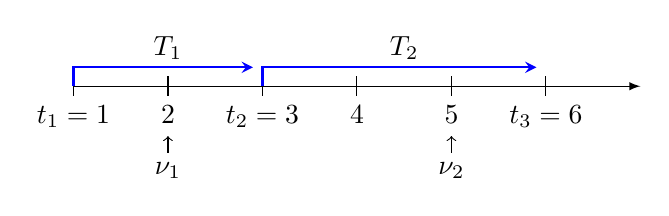
\begin{tikzpicture}[scale = 1.2]
    %\draw[latex-] (-1,0) -- (9,0) ;
    \draw[-latex] (1,0) -- (7,0) ;
    \foreach \x in  {1,2,3,4,5,6} \draw[shift={(\x,0)},color=black] (0pt,3pt) -- (0pt,-3pt);
    \foreach \x\xtext in {1/$t_1=1$,2,3/$t_2=3$,4,5,6/$t_3=6$} \draw[shift={(\x,0)},color=black] (0pt,0pt) -- (0pt,-3pt)
    node[below] {\xtext};
    \draw ; \node[] at (2,0.4) {$T_1$};
    \draw ; \node[] at (4.5,0.4) {$T_2$};
    
    %\draw[->] (0, -20 pt)node[below]{$t_0$} -- (0,-10pt); 
    %\draw[->] (1, -20 pt)node[below]{$t_1$} -- (1,-10pt);
    %\draw[->] (3, -20 pt)node[below]{$t_2$} -- (3,-10pt);
    %\draw[->] (6, -20 pt)node[below]{$t_3$} -- (6,-10pt);
    
    \draw[->] (2, -20 pt)node[below]{$\nu_1$} -- (2,-15pt);
    \draw[->] (5, -20 pt)node[below]{$\nu_2$} -- (5,-15pt);
    
    
    %\draw[blue]node[above]{$T_0$}(0.5,0)
    
    \draw [blue, thick, -stealth] (1,0) |- (2.9,0.2);
    \draw [blue, thick, -stealth] (3,0) |- (5.9,0.2);
    
    \end{tikzpicture}
    \caption{Infusing noise for enhanced exploration}
    \label{fig:horizon}
\end{figure}


\begin{algorithm}[h]
\caption{Thompson sampling with Langevin dynamics for LQR
}
\label{alg:ula}
\begin{algorithmic}[1]
\State {\bf Input:} $p_1$;
\State {\bf Initialization:} $t \leftarrow 1$, $t_0 \leftarrow 0$,
$x_1 \leftarrow 0$, $\mathcal{D} \leftarrow \emptyset$,
$\mathbf{U}_0 \leftarrow U_1$,
$\tilde{{\theta}}_0 \leftarrow \argmin U_1 (\theta)$, $\theta_{\min, 0} \leftarrow \tilde{\theta}_0$;
\For{Episode $k = 1,2,\ldots$}
\State $T_{k} \leftarrow k+1$, and $t_k \leftarrow t$;
%\STATE \textbf{\#Updating the potential for posterior}\\
\State $\mathbf{U}_k (\cdot) := \mathbf{U}_{k-1} (\cdot) -\sum_{(z_t, x_{t+1}) \in \mathcal{D}} \log p_w(x_{t+1} -\Theta^\top z_t)$;
\State $\mathcal{D} \leftarrow \emptyset$;
%\STATE \textbf{\# Approximate posterior sampling via preconditioned ULA}\\
\State $\theta_{\min, k} \in \argmin \mathbf{U}_k (\theta)$;
\State Compute the preconditioner $\tilde{P}_k$, the step  size $\tilde{\gamma}_k$, and the number of iterations $\tilde{N}_k$;
\While{True}
\State ${\theta}_0 \leftarrow \theta_{\min, k}$;
\For{Step $j=0, 1, \ldots, \tilde{N}_k-1$}
\State Sample ${\theta}_{j+1}$ according to \eqref{ULAstep};
\EndFor

\If{$\theta_{\tilde{N}_k} \in \mathcal{C}$}
\State $\tilde\theta_k\leftarrow\theta_{\tilde{N}_k}$
\State Break;
\EndIf

\EndWhile
\State Compute the gain matrix $K_k := K(\tilde{\theta}_k)$;
\While{ $t \leq t_k + T_{k}-1$}
\State Execute control $u_t = K_k x_t + \nu_t$ for $\nu_t$ satisfying Assumption~\ref{ass:perturb};
\State Observe new state $x_{t+1}$, and update $\mathcal{D} \leftarrow \mathcal{D} \cup \{(z_t, x_{t+1})\}$;
\State  $t \leftarrow t+1$;
\EndWhile
\EndFor
\end{algorithmic}
\end{algorithm}


One of the novel components in our algorithm is the injection of a noise signal into the control input $u_t$ at the end of each episode as illustrated in Figure~\ref{fig:horizon}. 
This perturbation enhances exploration.
The external noise signal is assumed to satisfy the following properties.

\begin{assumption}\label{ass:perturb}
The  $\bar L_\nu$-sub-Gaussian\footnote{A distribution is $L_\nu$-sub-Gaussian if $\mathrm{Pr}(|\nu| > y )< C  \text{exp}(-\frac{1}{2L_{\nu}^2} y^2)$ for some $C>0$.} random variable $\nu_{s} \in \mathbb{R}^{n_u}$ satisfies $\nu_s=0$ if $s\in [t_j,t_{j+1}-2]$ for all $j\geq 2$. Furthermore, $\mathbb{E}[\nu_s]=0$ and $\mathbf{W}':=\mathbb{E}[\nu_s \nu_s^{\top}]$ is a positive definite matrix whose maximum and minimum eigenvalues are identical to those of $\mathbf{W}$, the covariance matrix of $w_t$.\footnote{The assumption on the minimum eigenvalue of $\mathbf{W'}$ is needed just for simplicity in the proof of Proposition~\ref{prop:pers-ex} which is about the growth of $\lambda_{\min}(P_t)$.} 
\end{assumption}



Our proposed algorithm is presented in Algorithm~\ref{alg:ula}.
Here, $t_k$ and $T_k$ denote the start time and the length of episode $k$ respectively. By  definition, $t_1=1$ and $t_{k+1} = t_k + T_k$. The length of episode $k$ is chosen as $T_k = k+1$.
To update the posterior, or equivalently, its potential at episode $k$, we use the dataset $\mathcal{D}:= \{(z_t, x_{t+1})\}_{t_{k-1} \leq t \leq t_{k} - 1}$ collected during the previous episode. 
It follows from \eqref{posterior} that the potential can be updated  as Line 5,
where $\mathbf{U}_0$ is set to be  $U_1$, the potential of the prior.

Having the posterior updated, approximate TS is performed using the preconditioned ULA. 
The preconditioner, stepsize, and number of iterations are chosen as $\tilde{P}_{k}= {P}_{t_k}$, $\tilde{\gamma}_k={\gamma}_{t_k}$ and $\tilde{N}_k={N}_{t_k}$, where
\begin{equation}\label{preconditioner_stepsize_iteration}
     \begin{split}
     &{P}_{t}:=\lambda I_{dn} + \sum_{s=1}^{t-1} \mathrm{blkdiag}\{z_sz_s^\top\}_{i=1}^n, \; {\gamma}_t := \frac{m \lambda_{\min,t}}{16 M^2 \max\{\lambda_{\min,t},t \}}, \;  {N}_t := \frac{4\log_2 (\frac{\max\{\lambda_{\min,t},t\}}{\lambda_{\min,t}})}{m \gamma_t},
     \end{split}
\end{equation}
where $\theta_{\min, t}$ is a minimizer of the potential $U_t$, and $\lambda_{\min,t}$ and $\lambda_{\max,t}$ are the minimum and maximum eigenvalues of ${P}_t$. In the algorithm, we achieve the unique minimizer $\theta_{\min, t}$ by the Newton's method.

Accordingly, the update rule~\eqref{preULA} for the preconditioned ULA is expressed as
\begin{equation}\label{ULAstep}
\theta_{j+1} \sim \mathcal{N} ( \theta_j - \tilde{\gamma}_k \tilde{P}_k^{-1} \nabla \mathbf{U}_k (\theta_j), 2\tilde{\gamma}_k \tilde{P}_k^{-1}).
\end{equation}
After preforming the update $\tilde{N}_k$ times, we check whether $\theta_{N_k}$ is contained in $\mathcal{C}$. 
If so, the sampled parameter is accepted and the corresponding control gain matrix for the $k$th episode is computed using Theorem~\ref{lqr}.
This controller is then executed to collect transition data and the input is perturbed at the last step of the episode via the external noise signal $\nu_t$. 


\section{Concentration properties}

To show that Algorithm~\ref{alg:ula} achieves an $O(\sqrt{T})$ regret bound, 
we first examine the concentration properties of the exact and approximate posterior distributions given a history up to time $t$ for the potential $U_t(\theta)=U_1(\theta) - \sum_{s=1}^{t-1} \log p_w(x_{s+1}-\Theta^\top z_s)$ for a fixed $t$. When $t$ is chosen as $t_k$, we recover the case of Algorithm~\ref{alg:ula}.
As illustrated in Figure~\ref{fig:flow}, 
the concentration properties identified in this section enable us to bound the moments of the system state and attain the desired regret bound in Section~\ref{sec:regret}. 


\begin{figure*}[h]
\centering
\tikzstyle{concentration} = [rectangle, rounded corners, 
minimum width=1.5cm, 
minimum height=1.5cm,
text centered, 
draw=black, 
fill=white!30]

\tikzstyle{excitation} = [rectangle, rounded corners, 
minimum width=1.5cm, 
minimum height=1.5cm,
text centered, 
draw=black, 
fill=white!30]

\tikzstyle{state} = [rectangle, rounded corners, 
minimum width=1.5cm, 
minimum height=1.5cm,
text centered, 
draw=black, 
fill=white!30]

\tikzstyle{etc} = [rectangle, rounded corners, 
minimum width=1.5cm, 
minimum height=1.5cm,
text centered, 
draw=black, 
fill=white!30]

\tikzstyle{main} = [rectangle, rounded corners, 
minimum width=1.5cm, 
minimum height=1.5cm,
text centered, 
draw=black, 
fill=white!30]

\tikzstyle{io} = [trapezium, 
trapezium stretches=true, % A later addition
trapezium left angle=70, 
trapezium right angle=110, 
minimum width=3cm, 
minimum height=1cm, text centered, 
draw=black, fill=blue!30]

\tikzstyle{process} = [rectangle, 
minimum width=3cm, 
minimum height=1cm, 
text centered, 
text width=3cm, 
draw=black, 
fill=orange!30]

\tikzstyle{decision} = [diamond, 
minimum width=3cm, 
minimum height=1cm, 
text centered, 
draw=black, 
fill=green!30]
\tikzstyle{arrow} = [thick,->,>=stealth]


\begin{tikzpicture}[node distance=2.5cm,font=\sffamily\scriptsize]

\node (state_poly) [state] 
{\begin{tabular}{c}
    Theorem ~\ref{thm:state_poly}: \\
    Polynomial time
    bound\\ for  system state
\end{tabular}};

\node (concent_prob) [concentration, above of = state_poly, yshift=-0.5cm] {\begin{tabular}{c}
    Prop. ~\ref{prop:ula} \& Prop. ~\ref{prop:half_exact_true}:\\
    Comparison between\\ exact and approximate\\ posteriors
\end{tabular}};



\node (concent) [concentration, right of=state_poly, xshift= 1.25cm]
{\begin{tabular}{c}
    Theorem ~\ref{thm:exact_appox}: \\
    Concentration of\\  approximate posteriors
    \end{tabular}};

\node (per_ex) [excitation, above of=concent, yshift=-0.5cm]
{\begin{tabular}{c}
    Prop. ~\ref{prop:pers-ex}:\\
    Decay of $\frac{1}{\lambda_{\min,t}}$\\
    as $t\rightarrow\infty$
\end{tabular}};


\node (state_bound) [state, right of=concent,xshift= 1cm]
{\begin{tabular}{c}
    Theorem ~\ref{thm:improved}: \\  
    Bounding\\ the moments of\\  system state
\end{tabular}};
\node (regret) [main, right of=state_bound,xshift= 1cm] 
{\begin{tabular}{c}
    Theorem ~\ref{thm:regret}:\\ Regret bound\\  
    $R(T) \leq O(\sqrt{T})$
\end{tabular}};
\node (bellman) [etc, above of=regret,yshift= -0.5cm] 
{\begin{tabular}{c}
    Bellman's principle  
\end{tabular}};

\draw [arrow] (concent_prob) -- (state_poly);
%\draw [arrow] (state_poly) -- (per_ex);
\draw [arrow] (state_poly) -- (concent);
%\draw [arrow] (state_poly) .. controls +(down:2mm) and  +(down:2mm) .. (state_bound);
\draw [arrow] (state_poly.south) to [out=-10,in=-170] (state_bound.south);
\draw [arrow] (per_ex) -- (concent);
\draw [arrow] (concent) -- (state_bound);
\draw [arrow] (state_bound) -- (regret);
\draw [arrow] (bellman) -- (regret);
\end{tikzpicture}
\caption{Flow chart of our theoretical results.}\label{fig:flow}
\end{figure*}



\subsection{Comparing exact and approximate posteriors}

Let $\mu_t$ denote the \emph{exact posterior} distribution defined by $\mu_t \sim \exp (-U_t)$.
Regarding the approximate posterior, recall the preconditioned ULA that generates
$\theta_{j+1} \sim \mathcal{N} ( \theta_j - \gamma_t P_t^{-1} \nabla U_t (\theta_j), 2\gamma_t P_t^{-1})$ for $\theta_0 \in  \argmin U_t (\cdot)$.
Repeating this update $N_t$ times yields $\theta_{N_t}$.
We let $\tilde{\mu}_t$ denote the \emph{approximate posterior} defined as the distribution of $\theta_{N_t}$. 
We first compare the exact and approximate posteriors. 
The result quantifies the concentration depending on the moment $p$. The higher moment bound for $p>2$ is used to characterize a set of system parameters with which the state does not grow exponentially as illustrated in the following subsection, while the bound for $p=2$ is necessary for our regret analysis.
Throughout the paper, the joint distribution between $\mu_t$ and $\tilde \mu_t$ is given by the shared Brownian motion as demonstrated in Remark~\ref{rem:shared}.
\begin{prop}\label{prop:ula}
Suppose Assumptions~\ref{ass:noise} and~\ref{ass:init_bound} hold. 
Given any trajectory $(z_s)_{s\geq1}$, the exact posterior $\mu_t$ and the approximate posterior $\tilde{\mu}_t$ obtained by preconditioned ULA satisfy 
\[
\mathbb{E}_{\theta_t \sim \mu_t, \tilde{\theta}_t \sim \tilde{\mu}_t}\big[
| \theta_t - \tilde{\theta}_t |^p_{P_t} \mid h_{t}
\big ] \leq D_p
\]
for $p\geq 2$,
where $D_p = \big(\frac{pdn}{m}\big)^{\frac{p}{2}}\big(2^{2p+1}+5^p\big)$. When $p=2$, we further have
\begin{equation}\label{bd:comp}
\mathbb{E}_{\theta_t \sim \mu_t, \tilde{\theta}_t \sim \tilde{\mu}_t}\big[
| \theta_t - \tilde{\theta}_t |^2 \mid h_{t}
\big ]^{\frac{1}{2}} \leq \sqrt{\frac{D}{\max\{\lambda_{\min,t}, t\}}},
\end{equation}
where $D = 114\frac{dn}{m}$ and $\lambda_{\min,t}$ denotes the minimum eigenvalue of $P_t$.
\end{prop}

The proof of this proposition is contained in Appendix~\ref{app:prop:ula}.
If there were no preconditioner, it would be inevitable to obtain a result weaker than Proposition~\ref{prop:ula}; Theorem~\ref{thm:naive_ula} would yield an $O({1}/{\sqrt{\lambda_{\min,t}}})$ rate of convergence, which is an LQR version of \cite[Theorem 5]{mazumdar2020thompson}.
To improve the rate of convergence, we infuse the timestep $t$ into the stepsize required for ULA so that the right-hand side of \eqref{bd:comp} decreases with $t$. 
Thus, $\max\{\lambda_{\min,t}, t\} \geq \lambda_{\min,t}$ contributes to achieving the better concentration property.

Another important observation is a probabilistic concentration bound for the exact posterior. 
This concentration property is essential in characterizing a confidence set to be used in the proof of Theorem~\ref{thm:state_poly}.
\begin{prop}\label{prop:half_exact_true}
Suppose Assumptions~\ref{ass:noise} and~\ref{ass:init_bound} hold. 
Given any trajectory $(z_s)_{s\geq1}$,
\begin{equation}
\begin{split}
    &\mathbb{E}_{\theta_t \sim \mu_t}\big[
    | \theta_t - \theta_* |^p_{P_t} \mid h_{t}
    \big ]^{\frac{1}{p}} \leq 2p \sqrt{\frac{8nM^2}{m^3}\log \bigg(\frac{n}{\delta}\bigg(\frac{\lambda_{\max,t}}{\lambda}\bigg)^{\frac{d}{2}}\bigg)+C}, \quad t >0
\end{split}
\end{equation}
holds with probability at least $1-\delta$ for
any $0<\delta < 1$ and $p \geq 2$, where
the constant $C>0$ depends only on $p$, $m$, $n$, $d$ and $\lambda$, and $\lambda_{\max,t}$ denotes the maximum eigenvalue of $P_t$.
\end{prop}

The proof of this proposition can be found in Appendix~\ref{app:prop:half_exact_true}.


\subsection{Bounding expected state norms by a polynomial of time}\label{sec:polystate}

A nontrivial result we can derive from Propositions~\ref{prop:ula} and~\ref{prop:half_exact_true} is that the system state has a polynomial-time growth in expectation. 
To show this property, we modify the confidence set and self-normalization technique developed for the OFU approach~\cite{abbasi2011improved,abbasi2011regret}.
Our key idea is to construct a set containing sampled system parameters obtained by ULA with high probability.
The higher moment bounds from Propositions~\ref{prop:ula} and ~\ref{prop:half_exact_true} are crucial for our analysis as Markov-type inequalities can be exploited for any power $p$. We then split the probability space of the stochastic process into two sets, ``good'' and ``bad'', as in the OFU approach.

\begin{thm}\label{thm:state_poly}
Suppose that Assumption \ref{ass:noise},\ref{ass:init_bound} and \ref{ass:perturb} hold.
For $T >0$, $p\geq 2$ and any trajectory $(x_s)_{s=1}^T$ generated by Algorithm~\ref{alg:ula}, we have
\[
\mathbb{E} \Big [\max_{j\leq t}|x_j|^p  \Big ] \leq Ct^{\frac{7}{2}p(d+1)}, \quad t \geq 1,
\]
where the constant $C>0$ depends only on $p$, $m$, $n$, $n_u$, $\bold{W}$, $M_\rho$ and $\lambda$ in Assumption~\ref{ass:init_bound}. 
\end{thm}

The proof of this theorem can be found in Appendix~\ref{app:polystate}.
It is worth emphasizing that this polynomial time bound is attained without using predefined sets of parameters that make the true system stabilizable. 
In Section~\ref{sec:regret}, we will further improve the result to a uniform bound, which plays a critical role in our regret analysis. 



Leveraging the previous results on the concentration and the expected state norms, we can deduce that the minimum eigenvalue of the preconditioner actually grows in time. 
With this property as well as Theorem~\ref{thm:state_poly}, an improved concentration property of the exact posterior follows. Finally, the triangle inequality yields the desired result, the concentration of the approximate posterior around the true system parameter.

We begin by characterizing the growth of the minimum eigenvalue of the preconditioner which comes from the implementation of a random noise signal $\nu_s$ to perturb the action at the end of each episode.
To obtain this result, we decompose the preconditioner in each episode into two parts, a random matrix and a self-normalized matrix value process as in~\cite{jedra2022minimal}. 
Specifically, by Lemma~\ref{lem:preconditioner_expansion}, 
\begin{equation}\nonumber
\begin{split}
&\sum z_s z_s^\top=\sum  \underbrace{(L_s\psi_s)(L_s\psi_s)^{\top}}_{\text{random matrix part}} - \underbrace{(\sum  y_s (L_s \psi_s)^{\top})^{\top}(\sum y_sy_s^{\top}+  I_d)^{-1}(\sum   y_s (L_s \psi_s)^{\top})}_{\text{self-normalization}} -  I_d,
\end{split}
\end{equation}
where $y_s := 
\begin{bmatrix}
    A_*x_{s-1} + B_*u_{s-1}          \\
    K_j(A_*x_{s-1} + B_*u_{s-1})
\end{bmatrix}$, 
$L_s := 
\begin{bmatrix}
    I_n & 0\\
    K_j & I_{n'}
\end{bmatrix}$,
 $\psi_s :=
\begin{bmatrix}
    w_{s-1}\\
    \nu_{s}
\end{bmatrix}$, and $K_j$ is  the control gain matrix for the $j$th episode.
The random matrix part is indeed a sum of random matrices, and thus they contribute to accumulating the minimum eigenvalue of the preconditioner with high probability.
By Theorem~\ref{thm:state_poly}, the self-normalization term is bounded by $O(\log T)$ with high probability.
More rigorously, the following proposition holds:

\begin{prop}\label{prop:pers-ex}
Suppose that Assumptions \ref{ass:noise}--\ref{ass:perturb} hold. For  $k\geq k_0(m,n,n_u,\lambda,M_K,M_\rho,\mathbf{W})$, we have
\[
\mathbb{E}\bigg[\frac{1}{\lambda_{\min,t_{k+1}}^p}\bigg] \leq C k^{-p}, \quad p\geq 2,\] where $t_{k+1}$ is the start time of episode $k+1$ in Algorithm~\ref{alg:ula}, 
$\lambda_{\min, t_{k+1}}$ denotes the minimum eigenvalue of $\tilde{P}_{k+1} = P_{t_{k+1}}$ and the constant $C > 0$ depends only on $p, n, n_u, \bold{W}, M_K$ and $\lambda$  in Assumption~\ref{ass:init_bound}.
\end{prop}

The proof of this proposition can be found in Appendix~\ref{app:prop:pers-ex}.
Recalling the probabilistic bound for $|\theta_t - \theta_*|_{P_t}$ from Proposition~\ref{prop:half_exact_true}, 
we deduce that 
$|\theta_t - \theta_* |$ is controlled by  $1/\sqrt{\lambda_{\min,t}}$ and self-normalization term.
Using Theorem~\ref{thm:state_poly}, we can show that the latter is dominated by the former, which has a polynomial-time growth due to Proposition~\ref{prop:pers-ex}. 
Consequently, the following improved concentration bound holds for the exact posterior.

\begin{thm}\label{thm:exact_appox}
Suppose that Assumptions \ref{ass:noise}--\ref{ass:perturb} hold. Then, the exact posterior $\mu_{t}$ and approximate posterior $\tilde \mu_t$ realized from the shared Brownian motion satisfy
\[
\mathbb{E}\big [\mathbb{E}_{\theta_t \sim \mu_{t}}[|\theta_t-\theta_*|^p \mid h_{t}] \big ] \leq C\Big(t^{-\frac{1}{4}}\sqrt{\log t}\Big)^p, \mbox{ and }
\mathbb{E}\big[\mathbb{E}_{\tilde{\theta}_t \sim \tilde{\mu}_t}[| \tilde{\theta}_t - \theta_* |^p \mid h_{t} ]\big] \leq C\Big(t^{-\frac{1}{4}}\sqrt{\log t}\Big)^p
\] 
for all $t\geq 1$ and $p\geq 2$, where  the constant $C > 0$ depends only on $p, n, n_u, \bold{W}$, $M_K$, $M_\rho$, and $\lambda$  in Assumption~\ref{ass:init_bound}.
\end{thm}

The proof of this theorem can be found in Appendix~\ref{app:thm:exact_appox}.


\subsection{Concentration of exact and approximate posteriors}


Leveraging the previous results on the concentration and the expected state norms, we can deduce that the minimum eigenvalue of the preconditioner actually grows in time. 
With this property as well as Theorem~\ref{thm:state_poly}, an improved concentration property of the exact posterior follows. Finally, the triangle inequality yields the desired result, the concentration of the approximate posterior around the true system parameter.

We begin by characterizing the growth of the minimum eigenvalue of the preconditioner which comes from the implementation of a random noise signal $\nu_s$ to perturb the action at the end of each episode.
To obtain this result, we decompose the preconditioner in each episode into two parts, a random matrix and a self-normalized matrix value process as in~\cite{jedra2022minimal}. 
Specifically, by Lemma~\ref{lem:preconditioner_expansion}, 
\begin{equation}\nonumber
\begin{split}
&\sum z_s z_s^\top=\sum  \underbrace{(L_s\psi_s)(L_s\psi_s)^{\top}}_{\text{random matrix part}} - \underbrace{(\sum  y_s (L_s \psi_s)^{\top})^{\top}(\sum y_sy_s^{\top}+  I_d)^{-1}(\sum   y_s (L_s \psi_s)^{\top})}_{\text{self-normalization}} -  I_d,
\end{split}
\end{equation}
where $y_s := 
\begin{bmatrix}
    A_*x_{s-1} + B_*u_{s-1}          \\
    K_j(A_*x_{s-1} + B_*u_{s-1})
\end{bmatrix}$, 
$L_s := 
\begin{bmatrix}
    I_n & 0\\
    K_j & I_{n'}
\end{bmatrix}$,
 $\psi_s :=
\begin{bmatrix}
    w_{s-1}\\
    \nu_{s}
\end{bmatrix}$, and $K_j$ is  the control gain matrix for the $j$th episode.
The random matrix part is indeed a sum of random matrices, and thus they contribute to accumulating the minimum eigenvalue of the preconditioner with high probability.
By Theorem~\ref{thm:state_poly}, the self-normalization term is bounded by $O(\log T)$ with high probability.
More rigorously, the following proposition holds:

\begin{prop}\label{prop:pers-ex}
Suppose that Assumptions \ref{ass:noise}--\ref{ass:perturb} hold. For  $k\geq k_0(m,n,n_u,\lambda,M_K,M_\rho,\mathbf{W})$, we have
\[
\mathbb{E}\bigg[\frac{1}{\lambda_{\min,t_{k+1}}^p}\bigg] \leq C k^{-p}, \quad p\geq 2,\] where $t_{k+1}$ is the start time of episode $k+1$ in Algorithm~\ref{alg:ula}, 
$\lambda_{\min, t_{k+1}}$ denotes the minimum eigenvalue of $\tilde{P}_{k+1} = P_{t_{k+1}}$ and the constant $C > 0$ depends only on $p, n, n_u, \bold{W}, M_K$ and $\lambda$  in Assumption~\ref{ass:init_bound}.
\end{prop}

The proof of this proposition can be found in Appendix~\ref{app:prop:pers-ex}.
Recalling the probabilistic bound for $|\theta_t - \theta_*|_{P_t}$ from Proposition~\ref{prop:half_exact_true}, 
we deduce that 
$|\theta_t - \theta_* |$ is controlled by  $1/\sqrt{\lambda_{\min,t}}$ and self-normalization term.
Using Theorem~\ref{thm:state_poly}, we can show that the latter is dominated by the former, which has a polynomial-time growth due to Proposition~\ref{prop:pers-ex}. 
Consequently, the following improved concentration bound holds for the exact posterior.

\begin{thm}\label{thm:exact_appox}
Suppose that Assumptions \ref{ass:noise}--\ref{ass:perturb} hold. Then, the exact posterior $\mu_{t}$ and approximate posterior $\tilde \mu_t$ realized from the shared Brownian motion satisfy
\[
\mathbb{E}\big [\mathbb{E}_{\theta_t \sim \mu_{t}}[|\theta_t-\theta_*|^p \mid h_{t}] \big ] \leq C\Big(t^{-\frac{1}{4}}\sqrt{\log t}\Big)^p, \mbox{ and }
\mathbb{E}\big[\mathbb{E}_{\tilde{\theta}_t \sim \tilde{\mu}_t}[| \tilde{\theta}_t - \theta_* |^p \mid h_{t} ]\big] \leq C\Big(t^{-\frac{1}{4}}\sqrt{\log t}\Big)^p
\] 
for all $t\geq 1$ and $p\geq 2$, where  the constant $C > 0$ depends only on $p, n, n_u, \bold{W}$, $M_K$, $M_\rho$, and $\lambda$  in Assumption~\ref{ass:init_bound}.
\end{thm}

The proof of this theorem can be found in Appendix~\ref{app:thm:exact_appox}.



\section{Regret bound} \label{sec:regret}

To further  improve the bound in Theorem~\ref{thm:state_poly}, we decompose the  moment of system state into two parts concerning the following cases: $|\tilde \theta_t-\theta_*|\leq \epsilon_0$ and $|\tilde \theta_t-\theta_*| > \epsilon_0$, where $\epsilon_0$ is a positive constant. 
When $\epsilon_0$ is small enough, 
we have $|A_*+B_*K(\tilde \theta_t)|<1$, and thus the first part can be easily handled. 
For the second part, we invoke the Markov inequality to balance out the growth of the state and the tail probability with an appropriate choice of $p$. 
This intuitive argument can be made rigorous using Theorems~\ref{thm:state_poly} and~\ref{thm:exact_appox} to obtain the following result. 

\begin{thm}\label{thm:improved}
Suppose that Assumptions \ref{ass:noise}-\ref{ass:perturb} hold.
For any $T > 0$ and any trajectory $(x_s)_{s=1}^T$ generated by Algorithm~\ref{alg:ula}, we have
\[
\mathbb{E} [|x_t|^q ] < C, \quad q = 2, 4,
\]
where  the constant $C >0$ depends only on $p, n, n_u, \bold{W}, M_K, M_\rho, \epsilon_0$, and $\lambda$. {Here, $\epsilon_0$ is a positive constant such that $|\theta - \theta_*| \leq \epsilon_0$ implies $|A_* + B_* K(\theta)| < 1$.} 
\end{thm}

The proof of this theorem can be found in Appendix~\ref{app:thm:improved}.

%\subsection{$O(\sqrt{T})$-regret bound}

Finally, we present our main result that Algorithm~\ref{alg:ula} achieves an $O(\sqrt{T})$ expected regret bound. 

\begin{thm}\label{thm:regret}
Suppose that Assumptions \ref{ass:noise}-\ref{ass:perturb} hold. Then, the expected cumulative regret~\eqref{regret} of Algorithm~\ref{alg:ula} is bounded as follows:
\[
R(T) \leq O(\sqrt{T}).
\]
\end{thm}
The proof of this theorem can be found in Appendix~\ref{app:thm:regret}.
The regret bound is empirically verified by the results of our experiments. See Appendix~\ref{app:exp} for our empirical analyses.



\section{Concluding remarks}
We proposed an efficient approximate TS algorithm for learning LQR with an  $O(\sqrt{T})$ regret bound. Our method does not require a prespecified set of stabilizing parameters or the independence of columns of $\Theta$. 
This relaxation of restrictive assumptions is enabled by 
a carefully designed preconditioned ULA as well as executing a perturbed control action only at the end of each episode.

Several directions for future research can be addressed. 
It seems possible to extend our algorithm to noises with non-log-concave potentials. As the log-concavity of the potential of posteriors is preserved even with the noises we consider, accelerating the sampling process was possible via preconditioning. To handle more general classes of noise, some different aspects of ULA should be explored. Recently,  \cite{cheng2018sharp} derived a sharp non-asymptotic rate of convergence of Langevin dynamics in a nonconvex setting. We expect to examine the incorporation of the result within our framework. 

\numberwithin{equation}{section}
 
\appendix

\section{Proofs}
\subsection{Proof of Theorem~\ref{thm:naive_ula}}\label{app:naive_ula}

To prove Theorem~\ref{thm:naive_ula}, we use the following lemma. 

\begin{lem}\label{lem:naive_ula}
Suppose Assumptions~\ref{ass:noise} holds.
Let $X \in \mathbb{R}^{n_x}$ be a random variable with probability density function $p(x) \propto e^{-U(x)}$, where $\lambda_{\min} I_{n_x}\preceq \nabla^2 U  \preceq  \lambda_{\max}I_{n_x}$
for $\lambda_{\max},\lambda_{\min}>0$. Let
$\{ Y_j\}$, $Y_j  \in \mathbb{R}^{n_x}$, be generated by the ULA as
\[
Y_{j+1} = Y_j - \gamma \nabla U(Y_j) + \sqrt{2\gamma} W_j,
\]
where $Y_0$ is a random variable with an arbitrary density function.
If  $\gamma \leq \frac{ \lambda_{\min}}{16\lambda_{\max}^2}$, then we have
\[
\mathbb{E} [ | Y_j - X |^2 ] < 2^{-\frac{\lambda_{\min}\gamma    j}{4}} \mathbb{E} [
| Y_0 - X |^2 
] + 
2^8 \frac{n_x \lambda_{\max}^2 }{\lambda_{\min}^2} \gamma,
\]
where $X$ and $Y_j$ are understood via the shared Brownian motion in continuous and discretized stochastic differential equations as demonstrated in Remark~\ref{rem:shared}.
\end{lem}

\begin{proof}
Let $\{Z_{\tau}\}_{\tau \geq 0}$ be a continuous interpolation of $\{Y_j\}$, defined by
\begin{equation}\label{eq:naive_sde_z}
\left \{
\begin{array}{ll}
\mathrm{d} Z_{\tau} = -  \nabla U(Y_j) \mathrm{d}{\tau} + \sqrt{2} \mathrm{d} B_{\tau}& \mbox{for }\tau \in [j\gamma, (j+1) \gamma) \\
Z_{\tau} = Y_j & \mbox{for } \tau = j\gamma.
\end{array}
\right.
\end{equation}
Note that $\lim_{\tau \nearrow j\gamma} Z_{\tau} = Y_j =  \lim_{\tau \searrow j\gamma} Z_{\tau}$ for each $j$, and thus $\{Z_{\tau}\}$ is a continuous process. 
We introduce another stochastic process $\{X_{\tau}\}$, defined by 
\[
\mathrm{d} X_{\tau} = - \nabla U( X_{\tau}) \mathrm{d} \tau + \sqrt{2} \mathrm{d} B_{\tau},
\]
where $X_0$ is a random variable with pdf $p(x) \propto e^{-U(x)}$.
By Lemma~\ref{lem:ld}, $X_{\tau}$ has the same pdf $p(x)$ for all $\tau$. 
We use the same Brownian motion $B_{\tau}$ to define both $\{Z_{\tau}\}$ and $\{X_{\tau}\}$. 
Fix an arbitrary $j$. 
Differentiating $|Z_{\tau} - X_{\tau}|^2$ with respect to $\tau \in [j\gamma, (j+1)\gamma)$ yields
\begin{equation}\nonumber
\begin{split}
\frac{\mathrm{d} |Z_{\tau} - X_{\tau}|^2}{\mathrm{d}{\tau}} &= 2(Z_{\tau} - X_{\tau})^\top \bigg (
\frac{\mathrm{d} Z_{\tau}}{\mathrm{d} {\tau}} - \frac{\mathrm{d} X_{\tau}}{\mathrm{d} {\tau}}
\bigg )\\
&= 2 (Z_{\tau} - X_{\tau})^\top ( - \nabla U (Y_j) +  \nabla U(Z_{\tau}))
+ 2 (Z_{\tau} - X_{\tau})^\top (  - \nabla U(Z_{\tau}) +  \nabla U(X_{\tau})).
\end{split}
\end{equation}
Therefore, we have
\begin{equation}\nonumber
\begin{split}
&2 (Z_{\tau} - X_{\tau})^\top ( - \nabla U (Y_j) + \nabla U(Z_{\tau}))
+ 2 (Z_{\tau} - X_{\tau})^\top (  -  \nabla U(Z_{\tau}) +  \nabla U(X_{\tau}))\\
&\leq 2 (Z_{\tau} - X_{\tau})^\top( - \nabla U (Y_j) +  \nabla U(Z_{\tau}))
- 2\lambda_{\min} (Z_{\tau} - X_{\tau})^\top  (Z_{\tau} - X_{\tau})\\
&\leq  2 |Z_{\tau} - X_{\tau}| |\nabla U(Z_{\tau}) - \nabla U (Y_j) |
-2 \lambda_{\min} |Z_{\tau} - X_{\tau}|^2,
\end{split}
\end{equation}
where the first inequality follows from the strong convexity of $U$.
On the other hand, using Young's inequality, we have 
\[
|Z_{\tau} - X_{\tau}|  |  \nabla U(Z_{\tau}) - \nabla U (Y_j) | 
\leq \frac{\lambda_{\min}| Z_{\tau} - X_{\tau}|^2}{2}  + \frac{|   \nabla U(Z_{\tau}) - \nabla U (Y_j) |^2}{2  \lambda_{\min}}.
\]
Combining all together, we deduce that
\[
\frac{\mathrm{d} |Z_{\tau} - X_{\tau}|^2}{\mathrm{d}{\tau}} \leq - \lambda_{\min}| Z_{\tau} - X_{\tau}|^2 + \frac{1}{\lambda_{\min}} |   \nabla U(Z_{\tau}) - \nabla U (Y_j) |^2,
\]
which implies 
\[
\frac{\mathrm{d}}{\mathrm{d} {\tau}} (e^{\lambda_{\min}  {\tau}} | Z_{\tau} - X_{\tau} |^2) \leq 
\frac{e^{\lambda_{\min} {\tau}}}{\lambda_{\min}} |   \nabla U(Z_{\tau}) - \nabla U (Y_j) |^2.
\]
Integrating both sides from $j\gamma$ to $(j+1)\gamma$ and then multiplying $e^{-\lambda_{\min} (j+1) \gamma}$, we have
\begin{align*}
| Z_{(j+1)\gamma} - X_{(j+1)\gamma} |^2 &\leq 
e^{-\lambda_{\min}  \gamma} | Z_{j\gamma} - X_{j\gamma} |^2\\
&\quad+\frac{1}{\lambda_{\min}} \int_{j\gamma}^{(j+1) \gamma} 
e^{-\lambda_{\min}( (j+1)\gamma - s)} |   \nabla U(Z_s) - \nabla U (Y_j) |^2 \mathrm{d} s.
\end{align*}
Since $X_t$ and $X$ have the same pdf, 
we have
\begin{align}
%\begin{split}
\mathbb{E} [| Z_{(j+1)\gamma} - X |^2 ] &\leq 
e^{-\lambda_{\min} \gamma} \mathbb{E} [ | Z_{j\gamma} - X |^2]
+\frac{1}{\lambda_{\min}} \int_{j\gamma}^{(j+1) \gamma} 
 \mathbb{E} [ | \nabla U(Z_s) - \nabla U (Y_j) |^2 ]\mathrm{d} s \nonumber\\
 &\leq e^{-\lambda_{\min}  \gamma} \mathbb{E} [ | Z_{j\gamma} - X |^2]
+\frac{\lambda_{\max}^2}{\lambda_{\min} } \int_{j\gamma}^{(j+1) \gamma} 
\mathbb{E} [ | Z_s-Y_j|^2 ] \mathrm{d} s,\label{eq:naive_bd}
\end{align}
where the first inequality follows from $e^{-\lambda_{\min} ( (j+1)\gamma - s)}  \leq 1$ and the second inequality follows from the Lipschitz smoothness of $U$.

To bound~\eqref{eq:naive_bd}, we handle its first and second terms   separately. 
Regarding the second term, we first integrate the SDE \eqref{eq:naive_sde_z} from $j\gamma$ to $s \in [j \gamma, (j+1)\gamma )$  to obtain 
\begin{equation}\nonumber
 Z_s - Y_j   =    -(s - j\gamma)  \nabla U(Y_j) + \sqrt{2} (B_s - B_{j\gamma}).  
\end{equation}
The second term of \eqref{eq:naive_bd} can then be bounded  by
\begin{equation}\label{eq:naive_bd0}
\begin{split}
&\int_{j\gamma}^{(j+1) \gamma} 
\mathbb{E} [ | Z_s-Y_j|^2 ] \mathrm{d} s 
= \int_{j\gamma}^{(j+1) \gamma}\mathbb{E} [ | 
-(s - j\gamma)  \nabla U(Y_j) + \sqrt{2} (B_s - B_{j\gamma})
|^2 ] \mathrm{d} s \\
&\leq 2\bigg [
 \int_{j\gamma}^{(j+1) \gamma} \mathbb{E} [ | 
(s - j\gamma)  \nabla U(Y_j) |^2] \mathrm{d} s
+ 2 \int_{j\gamma}^{(j+1) \gamma} \mathbb{E} [|B_s - B_{j\gamma} |^2] \mathrm{d}s \bigg ].
\end{split}
\end{equation}
For $s \in [j\gamma, (j+1) \gamma)$, we note that $|s - j\gamma| \leq \gamma$, and thus
\begin{equation}\label{eq:naive_bd1}
\begin{split}
\int_{j\gamma}^{(j+1) \gamma} \mathbb{E} [ | 
(s - j\gamma)  \nabla U(Y_j) |^2] \mathrm{d} s
&\leq \gamma^2 \int_{j\gamma}^{(j+1) \gamma}  \mathbb{E} [
| \nabla U(Y_j) |^2 
] \mathrm{d} s \\
&= \gamma^3 \mathbb{E} [
| \nabla U(Y_j) |^2
] \\
&= \gamma^3 \mathbb{E} [
| \nabla U(Y_j) -  \nabla U(x_{\min}) |^2
]  \\
&\leq \gamma^3 \lambda_{\max}^2  \mathbb{E} [ | Y_j - x_{\min} |^2 ], 
\end{split}
\end{equation}
where $x_{\min}$ is a minimizer of  $U$.
It follows from  \cite[Lemma 10]{mazumdar2020thompson} that
\begin{equation}\label{eq:naive_bd2}
\begin{split}
\mathbb{E} [ | Y_j - x_{\min}|^2] & \leq 2\mathbb{E} [ | Y_j - X|^2] + 10^2 \frac{n_x}{\lambda_{\min}}.
\end{split}
\end{equation}
Moreover,  \cite[Lemma 8]{mazumdar2020thompson} yields
\begin{equation}\label{eq:naive_bd3}
\int_{j\gamma}^{(j+1)\gamma} \mathbb{E} [
| B_s - B_{j\gamma}|^2
]\mathrm{d}s \leq \frac{4n_x}{e} \gamma^2.
\end{equation}

Combining \eqref{eq:naive_bd0}--\eqref{eq:naive_bd3}, we obtain that 
\begin{equation}\nonumber
\begin{split}
\int_{j\gamma}^{(j+1)\gamma} \mathbb{E} [
| Z_s - Y_j |^2
]\mathrm{d} s &\leq 
2^2 \lambda_{\max}^2 \gamma^3 \mathbb{E} [ | Y_j - X |^2 ] + 2(10 \lambda_{\max})^2 \gamma^3 \frac{n_x}{\lambda_{\min}} +  \frac{16n_x}{e}\gamma^2\\
&\leq 2^2 \lambda_{\max}^2 \gamma^3 \mathbb{E} [ | Y_j - X |^2 ] + 2^5 n_x \gamma^2,
\end{split}
\end{equation}
where the second inequality follows from $\gamma \leq \frac{\lambda_{\min}}{16 \lambda_{\max}^2}$. 



Substituting this bound into \eqref{eq:naive_bd}, we have
\begin{equation}\nonumber
\begin{split}
\mathbb{E} [| Z_{(j+1)\gamma} - X |^2 ]  &< e^{-\lambda_{\min}  \gamma} \mathbb{E} [ | Z_{j\gamma} - X |^2]
+2^2\frac{\lambda_{\max}^4}{\lambda_{\min}} \gamma^3 \mathbb{E} [ | Y_j - X |^2 ]
+ 2^5 n_x \frac{\lambda_{\max}^2}{\lambda_{\min}} \gamma^2\\
&\leq  \bigg (
1 - \frac{\lambda_{\min} }{4}\gamma
\bigg )^2 \mathbb{E} [ | Y_j - X|^2]+2^2\frac{\lambda_{\max}^4}{\lambda_{\min}} \gamma^3 \mathbb{E} [ | Y_j - X |^2 ]
+ 2^5 n_x \frac{\lambda_{\max}^2}{\lambda_{\min} } \gamma^2,
\end{split}
\end{equation}
where the second inequality follows from the fact that 
$e^{-x} \leq 1 - \frac{x}{2}$ for $x \in [0,1]$. 
To further simplify the upper-bound, we use the following  two inequalities: 
$2^2\frac{\lambda_{\max}^4}{\lambda_{\min}} \gamma^3 = \frac{\lambda_{\min}}{64 } \big (\frac{16 \lambda_{\max}^2}{\lambda_{\min}}\big )^2\gamma^3 
\leq \frac{\lambda_{\min}}{64 }  \gamma$ and 
$\big (
1 - \frac{\lambda_{\min}}{4}\gamma
\big )^2 + \frac{\lambda_{\min}}{64}  \gamma \leq \big (
1 - \frac{\lambda_{\min}}{8}\gamma
\big )^2$.
Consequently, $\mathbb{E} [| Z_{(j+1)\gamma} - X |^2 ]$ is bounded as
\[
\mathbb{E} [| Z_{(j+1)\gamma} - X |^2 ] < \bigg (
1 - \frac{\lambda_{\min} }{8}\gamma
\bigg )^2\mathbb{E} [ | Y_j - X|^2]  + 2^5 n_x \frac{\lambda_{\max} ^2}{\lambda_{\min} } \gamma^2.
\]
Invoking this inequality repeatedly yields
\begin{equation}\nonumber
\begin{split}
\mathbb{E} [| Z_{(j+1)\gamma} - X |^2 ] &<
\bigg (
1 - \frac{\lambda_{\min} }{8}\gamma
\bigg )^{2(j+1)} \mathbb{E} [ | Y_0 - X|^2]
+ \sum_{i=0}^j \bigg (
1 - \frac{\lambda_{\min} }{8}\gamma
\bigg )^{2i} 2^5 n_x \frac{\lambda_{\max} ^2}{\lambda_{\min} } \gamma^2\\
&< \bigg (
1 - \frac{\lambda_{\min} }{8}\gamma
\bigg )^{2(j+1)} \mathbb{E} [ | Y_0 - X|^2]
+ \frac{1}{1 - (
1 - \frac{\lambda_{\min} }{8}\gamma
)}2^5 n_x \frac{\lambda_{\max} ^2}{\lambda_{\min} } \gamma^2\\
&= \bigg (
1 - \frac{\lambda_{\min} }{8}\gamma
\bigg )^{2(j+1)} \mathbb{E} [ | Y_0 - X|^2]
+ 2^8 n_x \frac{\lambda_{\max} ^2}{\lambda_{\min} ^2} \gamma.
%&\leq \bigg (
%1 - \frac{\lambda_{\min} }{8}\gamma
%\bigg )^{2(j+1)} \mathbb{E} [ | Y_0 - X|^2]
%+ 2^8 n_x \frac{\lambda_{\max} ^2}{\lambda_{\min}^2} \gamma.
\end{split}
\end{equation}
Since $(1 - \frac{\lambda_{\min} }{8} \gamma ) \leq (\frac{1}{2})^{\frac{\lambda_{\min} }{8} \gamma}$ and  $Z_{(j+1)\gamma} = Y_{j+1}$, we conclude that 
\[
\mathbb{E} [| Y_{j+1} - X |^2 ] = \mathbb{E} [| Z_{(j+1)\gamma} - X |^2 ] < \bigg (
\frac{1}{2}
\bigg )^{\frac{\lambda_{\min}\gamma (j+1) }{4}} \mathbb{E} [ | Y_0 - X|^2]
+ 2^8 n_x \frac{\lambda_{\max}^2 }{\lambda_{\min}^2} \gamma.
\]
Replacing $j+1$ with $j$, the result follows.
\end{proof}


\begin{proof}[Proof of Theorem ~\ref{thm:naive_ula}]

We now prove Theorem~\ref{thm:naive_ula}. It follows from  \cite[Lemma 10]{mazumdar2020thompson} that 
\[
\mathbb{E}_{x \sim p}\big[|x-x_{\min}|^2\big]^{\frac{1}{2}} \leq 5 \sqrt{\frac{2n_x}{\lambda_{\min}}},
\]
where $x_{\min}$ is a minimizer of $U$.
Using Lemma~\ref{lem:naive_ula} with $n_x = dn$ and 
the initial distribution $X_0 \sim \delta_{x_{\min}}$, we obtain that
\[
\mathbb{E}_{x \sim p, \tilde{x} \sim p_N}\big[|x-\tilde x|^2\big] < 2^{-\frac{\lambda_{\min} \gamma  N}{4}}
\mathbb{E}_{x \sim p}\big[|x-x_{\min}|^2\big] + 
2^8 \frac{n_x \lambda_{\max}^2}{ \lambda_{\min}^2 } \gamma.
\]
Taking the stepsize and the number of steps as 
$\gamma = \frac{\lambda_{\min}}{16\lambda_{\max}^2}$ and $N = \frac{64\lambda_{\max}^2}{\lambda_{\min}^2}$, respectively,
the first and second terms on the RHS of  the inequality above are bounded as
\begin{equation}\nonumber
\begin{split}
2^{-\frac{\lambda_{\min} \gamma  N}{4}}
\mathbb{E}_{x \sim p}\big[|x-x_{\min}|^2\big] &= 
\frac{1}{2} \mathbb{E}_{x \sim p}\big[|x-x_{\min}|^2\big]\leq 25 \frac{n_x}{\lambda_{\min}},
\end{split}
\end{equation}
and
\[
2^8 \frac{n_x \lambda_{\max}^2 }{\lambda_{\min}^2 } \gamma \leq 
2^4 \frac{n_x}{\lambda_{\min}},
\]
respectively. 
Therefore, we conclude that
\[
\mathbb{E}_{x \sim p, \tilde{x} \sim p_N}\big[|x-\tilde x|^2\big]^{\frac{1}{2}} < \sqrt{41\frac{n_x}{\lambda_{\min}}} = O\bigg (\sqrt{\frac{1}{\lambda_{\min}}} \bigg )
\]
as desired.
\end{proof}



\subsection{Proof of Lemma~\ref{concavity}}\label{app:sec_a}
\begin{proof}
By direct calculation, we first observe that
\begin{equation*}
    \nabla^2_{\theta} \log p_w(x_{s+1}-\Theta^\top z_s) = \nabla^2_{w_s} \log p_w(x_{s+1}-\Theta^\top z_s) \otimes z_s z_s^{\top},
\end{equation*}
where $\otimes$ denotes Kronecker product.
Then, the Hessian $\nabla^2_{\theta}U_t$ is given by 
\begin{equation*}
    \nabla^2_{\theta}U_t = \lambda I_{dn} - \sum_{s=1}^{t-1}\nabla^2_{w_s} \log p_w(x_{s+1}-\Theta^\top z_s) \otimes z_s z_s^{\top}.
\end{equation*} 
Under Assumption~\ref{ass:noise}, for any state action pair $z_s=(x_s,u_s)$, we have
\begin{equation*}
  \underline m\text{blkdiag}(\{ z_s z_s^{\top}\}_{i=1}^{n})   \preceq -\nabla^2_{w_s} \log p_w(x_{s+1}-\Theta^\top z_s) \otimes z_s z_s^{\top} \preceq \overline m \text{blkdiag}(\{z_s z_s^{\top}\}_{i=1}^{n}),
\end{equation*}
which implies that
\begin{equation*}
\begin{split}
   \min\{ \underline m, 1\}\bigg( \lambda I_{dn}+\sum_{s=1}^{t-1}\text{blkdiag}(\{z_s z_s^{\top}\}_{i=1}^{n})\bigg) &\preceq  \nabla^2_{\theta}U_t\\
   &\preceq \max\{ \overline m, 1\}\bigg( \lambda I_{dn}+\sum_{s=1}^{t-1}\text{blkdiag}(\{z_s z_s^{\top}\}_{i=1}^{n})\bigg). 
   \end{split}
   \end{equation*}
Finally, letting the preconditioner $P_t := \lambda I_{dn} +\sum_{s=1}^{t-1}\text{blkdiag}(\{z_s z_s^{\top}\}_{i=1}^{n})$, the result follows.
\end{proof}


\subsection{Proof of Proposition~\ref{prop:ula}}
\label{app:prop:ula}

To prove Proposition~\ref{prop:ula}, we first introduce the following two lemmas regarding the stationarity of the preconditioned Langevin diffusion and the non-asymptotic behavior of the preconditioned ULA. 

\begin{lem}\label{lem:ld}
Suppose that Assumptions~\ref{ass:noise} holds.
Let $X_{\tau} \in \mathbb{R}^{n_x}$ denote the solution of the preconditioned Langevin equation
\[
\mathrm{d} X_{\tau} = -P^{-1} \nabla U( X_{\tau}) \mathrm{d} {\tau} + \sqrt{2} P^{-\frac{1}{2}} \mathrm{d} B_{\tau},
\]
where $X_0$ is distributed according to $p(x) \propto e^{-U(x)}$, and 
 $P \in \mathbb{R}^{n_x \times n_x}$ is an arbitrary  positive definite matrix. 
Then, $X_{\tau}$ has the same probability density $p(x)$ for all ${\tau} \geq 0$. 
\end{lem}

\begin{proof}
Consider the following Fokker-Planck equation associated with the preconditioned Langevin equation:
\begin{equation}\label{fp}
\frac{\partial q (x, {\tau})}{\partial {\tau}} = -\sum_{i=1}^{n_x} \frac{\partial}{\partial x_i} \big ( 
[P^{-1} \nabla \log p (x) ]_i q (x, {\tau})
\big )
+ \sum_{i=1}^{n_x} \sum_{j=1}^{n_x} \frac{\partial^2}{\partial x_i \partial x_j} \big ( [P^{-1}]_{ij} q(x, {\tau})\big ).
\end{equation}
It is well known that $q(x,{\tau})$ is the probability density function of $X_{\tau}$. 
We can check that $p(x)$ is a solution of the Fokker-Planck equation by plugging $q(x, {\tau}) = p(x)$ into \eqref{fp}.
Specifically, 
\begin{equation}
\begin{split}
&-\sum_{i=1}^{n_x} \frac{\partial}{\partial x_i} \big ( 
[P^{-1} \nabla \log p (x) ]_i p(x) \big ) +  \sum_{i=1}^{n_x} \sum_{j=1}^{n_x} \frac{\partial^2}{\partial x_i \partial x_j} \big ( [P^{-1}]_{ij} p(x) \big )\\ &= 
-\sum_{i=1}^{n_x} \frac{\partial}{\partial x_i} \bigg ( \sum_{j=1}^{n_x}
[P^{-1}]_{ij} \frac{\partial}{\partial x_j} p (x)   \bigg) +  \sum_{i=1}^{n_x} \sum_{j=1}^{n_x} \frac{\partial^2}{\partial x_i \partial x_j} \big ( [P^{-1}]_{ij} p(x) \big ) = 
0 = \frac{\partial p(x)}{\partial {\tau}}.
\end{split}
\end{equation}
Since the Fokker-Planck equation has a unique smooth solution~\cite{pavliotis2014stochastic}, we conclude that $q(x, t) \equiv p(x)$ for all $t$, and the result follows. 
\end{proof}



\begin{lem}\label{lem:ula}
Suppose Assumptions~\ref{ass:noise} holds.
Let $X \in \mathbb{R}^{n_x}$ be a random variable with probability density function $p(x) \propto e^{-U(x)}$, and the stochastic process $\{ Y_j\}$, $Y_j  \in \mathbb{R}^{n_x}$, be generated by the preconditioned ULA as
\[
Y_{j+1} = Y_j - \gamma P^{-1} \nabla U(Y_j) + \sqrt{2\gamma P^{-1}} W_j,
\]
where $Y_0$ is a random variable with an arbitrary density function, and 
$P \in \mathbb{R}^{n_x \times n_x}$ is a positive definite matrix with minimum eigenvalue $\lambda_{\min}$ and maximum eigenvalue $\lambda_{\max}$.
If  $\gamma \leq \frac{m \lambda_{\min}}{16 M^2 \max\{\lambda_{\min},t\}}$ and  $m I_{n_x} \preceq P^{-\frac{1}{2}}\nabla^2U P^{-\frac{1}{2}}\preceq MI_{n_x}$, then we have  
\[
\mathbb{E} [ | Y_j - X |_P^p ] < \bigg (
\frac{1}{2}
\bigg )^{\frac{m \gamma (j+1) }{4}} \mathbb{E} [ | Y_0 - X|_P^p]
+ 2^{4p+1} (pn_x)^{\frac{p}{2}} \frac{M^p}{m^p} \gamma^{\frac{p}{2}}
\]
for any $p\geq 2$ where $X$ and $Y_j$ are understood via the shared Brownian motion in continuous and discretized stochastic differential equations as demonstrated in Remark~\ref{rem:shared}.
\end{lem}

\begin{proof}
Let $\{Z_{\tau}\}_{{\tau}\geq 0}$ be a continuous interpolation of $\{Y_j\}$, defined by
\begin{equation}\label{eq:sde_z}
\left \{
\begin{array}{ll}
\mathrm{d} Z_{\tau} = - P^{-1} \nabla U(Y_j) \mathrm{d}{\tau} + \sqrt{2P^{-1}} \mathrm{d} B_{\tau}& \mbox{for }{\tau} \in [j\gamma, (j+1) \gamma) \\
Z_{\tau} = Y_j & \mbox{for } {\tau} = j\gamma.
\end{array}
\right.
\end{equation}
Note that $\lim_{{\tau} \nearrow j\gamma} Z_{\tau} = Y_j =  \lim_{{\tau} \searrow j\gamma} Z_{\tau}$ for each $j$, and thus $\{Z_{\tau}\}$ is a continuous process. 
We introduce another stochastic process $\{X_{\tau}\}$, defined by 
\[
\mathrm{d} X_{\tau} = -P^{-1} \nabla U( X_{\tau}) \mathrm{d} {\tau} + \sqrt{2} P^{-\frac{1}{2}} \mathrm{d} B_{\tau},
\]
where $X_0$ is a random variable with pdf $p(x) \propto e^{-U(x)}$.
By Lemma~\ref{lem:ld}, $X_{\tau}$ has the same pdf $p(x)$ for all ${\tau}$. 
We use the same Brownian motion $B_{\tau}$ to define both $\{Z_{\tau}\}$ and $\{X_{\tau}\}$.

Fix an arbitrary $j$.
For any $p \geq 2$, 
differentiating $|Z_{\tau} - X_{\tau}|_P^p = |P^{\frac{1}{2}}(Z_{\tau} - X_{\tau})|^p$ with respect to ${\tau} \in [j\gamma, (j+1)\gamma)$, we have
\begin{align*}
\frac{\mathrm{d} |Z_{\tau} - X_{\tau}|_P^p}{\mathrm{d}{\tau}} &= p|P^{\frac{1}{2}}(Z_{\tau} - X_{\tau})|^{p-2}(Z_{\tau} - X_{\tau})^\top P \bigg (
\frac{\mathrm{d} Z_{\tau}}{\mathrm{d} {\tau}} - \frac{\mathrm{d} X_{\tau}}{\mathrm{d} {\tau}}
\bigg )
\\&= p|P^{\frac{1}{2}}(Z_{\tau} - X_{\tau})|^{p-2} (Z_{\tau} - X_{\tau})^\top ( - \nabla U (Y_j) +  \nabla U(Z_{\tau}))
\\& \quad + p|P^{\frac{1}{2}}(Z_{\tau} - X_{\tau})|^{p-2} (Z_{\tau} - X_{\tau})^\top (  - \nabla U(Z_{\tau}) +  \nabla U(X_{\tau})).
\end{align*}
Noting that $m  I_{n_x} \preceq P^{-\frac{1}{2}}\nabla^2 U P^{-\frac{1}{2}}  \preceq  M  I_{n_x}$, we have
\begin{equation}\nonumber
\begin{split}
&p|P^{\frac{1}{2}}(Z_{\tau} - X_{\tau})|^{p-2}\big[ (Z_{\tau} - X_{\tau})^\top ( - \nabla U (Y_j) + \nabla U(Z_{\tau}))
+ (Z_{\tau} - X_{\tau})^\top (  -  \nabla U(Z_{\tau}) +  \nabla U(X_{\tau}))\big]\\
&\leq p|P^{\frac{1}{2}}(Z_{\tau} - X_{\tau})|^{p-2} \big[(Z_{\tau} - X_{\tau})^\top P^{\frac{1}{2}} P^{-\frac{1}{2}}( - \nabla U (Y_j) +  \nabla U(Z_{\tau}))
- m (Z_{\tau} - X_{\tau})^\top P (Z_{\tau} - X_{\tau})\big]\\
&=p|P^{\frac{1}{2}}(Z_{\tau} - X_{\tau})|^{p-2}\big[  |Z_{\tau} - X_{\tau}|_P  |  P^{-\frac{1}{2}} \nabla U(Z_{\tau}) -P^{-\frac{1}{2}} \nabla U (Y_j) |
- m  |Z_{\tau} - X_{\tau}|_P^2\big],
\end{split}
\end{equation}
where the first inequality follows from the mean value theorem.
Now, recall the generalized Young's inequality, $ab \leq \frac{s^\alpha a^\alpha}{\alpha} + \frac{s^{-\beta}b^\beta}{\beta}$ for $s>0$, $a,b,\alpha,\beta>0$ such that $\frac{1}{\alpha}+\frac{1}{\beta}=1$.
Choosing $s=(\frac{pm}{2(p-1)})^{(p-1)/p}$, $\alpha=\frac{p}{p-1}$, and $\beta=p$ yields
\begin{align*}
&|Z_{\tau} - X_{\tau}|_P^{p-1}  |  P^{-\frac{1}{2}} \nabla U(Z_{\tau})) -P^{-\frac{1}{2}} \nabla U (Y_j) | \\
&\leq \frac{p-1}{p}\frac{pm}{2(p-1)} | Z_{\tau} - X_{\tau}|_P^p  + \frac{1}{p}\frac{1}{(\frac{pm}{2(p-1)})^{p-1}}|  P^{-\frac{1}{2}} \nabla U(Z_{\tau})) -P^{-\frac{1}{2}} \nabla U (Y_j) |^p.
\end{align*}
Combining all together with $\frac{pm}{2(p-1)}\geq \frac{m}{2}$, we have
\[
\frac{\mathrm{d} |Z_{\tau} - X_{\tau}|_P^p}{\mathrm{d}t} \leq - \frac{pm}{2}  | Z_{\tau} - X_{\tau}|_P^p + \frac{2^{p-1}}{m^{p-1}} |  P^{-\frac{1}{2}} \nabla U(Z_{\tau})) -P^{-\frac{1}{2}} \nabla U (Y_j) |^p,
\]
which implies that
\[
\frac{\mathrm{d}}{\mathrm{d} {\tau}} (e^{\frac{pm}{2}  {\tau}} | Z_{\tau} - X_{\tau} |_P^p) \leq 
e^{\frac{pm}{2}  {\tau}}\frac{2^{p-1}}{m^{p-1}} |  P^{-\frac{1}{2}} \nabla U(Z_{\tau})) -P^{-\frac{1}{2}} \nabla U (Y_j) |^p.
\]
Integrating both sides from $j\gamma$ to $(j+1)\gamma$ and then multiplying both sides by $e^{-\frac{pm}{2} (j+1) \gamma}$, we obtain that
\begin{align*}
&| Z_{(j+1)\gamma} - X_{(j+1)\gamma} |_P^p\\
&\leq 
e^{-\frac{pm}{2}  \gamma} | Z_{j\gamma} - X_{j\gamma} |_P^p
+\frac{2^{p-1}}{m^{p-1}} \int_{j\gamma}^{(j+1) \gamma} 
e^{-\frac{pm}{2} ( (j+1)\gamma - s)} |  P^{-\frac{1}{2}} \nabla U(Z_s)) -P^{-\frac{1}{2}} \nabla U (Y_j) |^p \mathrm{d} s.
\end{align*}
Since $X_{\tau}$ and $X$ have the same pdf due to Lemma~\ref{lem:ld}, we have
\begin{align}
%\begin{split}
&\mathbb{E} [| Z_{(j+1)\gamma} - X |^p_P ] \nonumber\\ &\leq 
e^{-\frac{pm}{2} \gamma} \mathbb{E} [ | Z_{j\gamma} - X |_P^p]
+\frac{2^{p-1}}{m^{p-1}} \int_{j\gamma}^{(j+1) \gamma} 
 \mathbb{E} [ |  P^{-\frac{1}{2}} \nabla U(Z_s)) -P^{-\frac{1}{2}} \nabla U (Y_j) |^p ]\mathrm{d} s \nonumber\\
 & = e^{-\frac{pm}{2} \gamma} \mathbb{E} [ | Z_{j\gamma} - X |_P^p]
+\frac{2^{p-1}}{m^{p-1}} \int_{j\gamma}^{(j+1) \gamma} 
 \mathbb{E} [ |  P^{-\frac{1}{2}} (\int_0^1 \nabla^2 U(Y_j + t(Y_j-Z_s))\mathrm{d}t)(Z_s-Y_j)  |^p ]\mathrm{d} s \nonumber\\
 & \leq e^{-\frac{pm}{2} \gamma} \mathbb{E} [ | Z_{j\gamma} - X |_P^p] \nonumber\\
&\quad +\frac{2^{p-1}}{m^{p-1}} \int_{j\gamma}^{(j+1) \gamma} 
 \mathbb{E} [ |  P^{-\frac{1}{2}} (\int_0^1 \nabla^2 U(Y_j + t(Y_j-Z_s))\mathrm{d}t)P^{-\frac{1}{2}}|^p|P^{\frac{1}{2}}(Z_s-Y_j)  |^p ]\mathrm{d} s \nonumber\\
 &\leq e^{-\frac{pm}{2}  \gamma} \mathbb{E} [ | Z_{j\gamma} - X |_P^p]
+\frac{2^{p-1}M^{p}}{m^{p-1}} \int_{j\gamma}^{(j+1) \gamma} 
\mathbb{E} [ | P^{\frac{1}{2}}(Z_s-Y_j) |^p ] \mathrm{d} s,\label{eq:bd}
%\end{split}
\end{align}
where the first inequality follows from $e^{-m ( (j+1)\gamma - s)}  \leq 1$ and the second inequality follows from the mean value theorem and the last inequality follows from the assumption in the lemma. 
To bound~\eqref{eq:bd}, we handle the first and second terms, separately. 

For the second term, we integrate \eqref{eq:sde_z} from $j\gamma$ to $s \in [j \gamma, (j+1)\gamma )$  to obtain 
\begin{equation} \nonumber
 Z_s - Y_j   =    -(s - j\gamma) P^{-1} \nabla U(Y_j) + \sqrt{2P^{-1}} (B_s - B_{j\gamma}).  
\end{equation}
Ignoring the constant coefficient, the second term of \eqref{eq:bd} is then bounded by
\begin{equation}\label{eq:bd0}
\begin{split}
&\int_{j\gamma}^{(j+1) \gamma} 
\mathbb{E} [ | P^{\frac{1}{2}}(Z_s-Y_j)|^p ] \mathrm{d} s 
\\
&= \int_{j\gamma}^{(j+1) \gamma}\mathbb{E} [ | 
-(s - j\gamma) P^{-\frac{1}{2}} \nabla U(Y_j) + \sqrt{2} (B_s - B_{j\gamma})
|^p ] \mathrm{d} s \\
&\leq 2^{p-1}\bigg [
 \int_{j\gamma}^{(j+1) \gamma} \mathbb{E} [ | 
(s - j\gamma) P^{-\frac{1}{2}} \nabla U(Y_j) |^p] \mathrm{d} s
+ 2^{\frac{p}{2}} \int_{j\gamma}^{(j+1) \gamma} \mathbb{E} [|B_s - B_{j\gamma} |^p] \mathrm{d}s \bigg ].
\end{split}
\end{equation}
For $s \in [j\gamma, (j+1) \gamma)$, we note that $|s - j\gamma| \leq \gamma$, and thus
\begin{equation}\label{eq:bd1}
\begin{split}
\int_{j\gamma}^{(j+1) \gamma} \mathbb{E} [ | 
(s - j\gamma) P^{-\frac{1}{2}} \nabla U(Y_j) |^p] \mathrm{d} s
&\leq \gamma^p \int_{j\gamma}^{(j+1) \gamma}  \mathbb{E} [
|P^{-\frac{1}{2}} \nabla U(Y_j) |^p
] \mathrm{d} s \\
&= \gamma^{p+1} \mathbb{E} [
|P^{-\frac{1}{2}} \nabla U(Y_j) |^p
] \\
&= \gamma^{p+1} \mathbb{E} [
|P^{-\frac{1}{2}} \nabla U(Y_j) - P^{-\frac{1}{2}} \nabla U(x_{\min}) |^p
]  \\
&\leq \gamma^{p+1} M^p  \mathbb{E} [ | Y_j - x_{\min} |_P^p ], 
\end{split}
\end{equation}
where $x_{\min}$ is a minimizer of potential $U$.

Let $\tilde{X} := P^{\frac{1}{2}}X$. Its pdf is denoted by by $ \tilde{p}(\tilde{x})$.
Then, for any $p\geq 2$,
\begin{equation}
\begin{split}
\mathbb{E} [ | Y_j - x_{\min}|_P^p] 
&\leq 2^{p-1} (
\mathbb{E} [ | Y_j - X|_P^p]
+\mathbb{E} [ | \tilde{X} - \tilde{x}_{\min}|^p]
),
\end{split}
\end{equation}
where $\tilde{x}_{\min} = P^{\frac{1}{2}} x_{\min}$. 
Since $\tilde{p}(\tilde{x}) = \det(P^{-\frac{1}{2}}) p (P^{-\frac{1}{2}}\tilde{x})$, we have
$-\nabla^2_{\tilde{x}} \log \tilde{p}(\tilde{x}) = -P^{-\frac{1}{2}} \nabla^2_x \log p(P^{-\frac{1}{2}}\tilde x) P^{-\frac{1}{2}}$.
Thus, $\tilde{p}$ is $m$-strongly log-concave. 
It follows from \cite[Lemma 10]{mazumdar2020thompson} that 
\begin{equation}\label{eq:bd2}
\begin{split}
\mathbb{E} [ | Y_j - x_{\min}|_P^p] & \leq 2^{p-1}\mathbb{E} [ | Y_j - X|_P^p] + \frac{10^p}{2} \big(\frac{pn_x}{m}\big)^{\frac{p}{2}}.
\end{split}
\end{equation}
On the other hand, \cite[Lemma 8]{mazumdar2020thompson} yields that
\begin{equation}\label{eq:bd3}
\int_{j\gamma}^{(j+1)\gamma} \mathbb{E} [
| B_s - B_{j\gamma}|^p
]\mathrm{d}s \leq 2\big(\frac{pn_x}{e}\big)^{\frac{p}{2}} \gamma^{\frac{p}{2}+1}.
\end{equation}
Combining \eqref{eq:bd0}--\eqref{eq:bd3}, we obtain that \begin{equation}
\begin{split}
&\int_{j\gamma}^{(j+1)\gamma} \mathbb{E} [
| Z_s - Y_j |_P^p
]\mathrm{d} s \\
&\leq 
2^{2p-2} M^p \gamma^{p+1} \mathbb{E} [ | Y_j - X |_P^p ] + 2^{p-2}(10 M)^p \gamma^{p+1} \big(\frac{pn_x}{m}\big)^{\frac{p}{2}} +  2^{\frac{3p}{2}}\big(\frac{pn_x}{e}\big)^{\frac{p}{2} }\gamma^{\frac{p}{2}+1}\\
&\leq 2^{2p-2} M^p \gamma^{p+1} \mathbb{E} [ | Y_j - X |_P^p ] + 2^{3p} (pn_x)^{\frac{p}{2}} \gamma^{\frac{p}{2}+1},
\\& 
\end{split}
\end{equation}
where the second inequality follows from $\gamma \leq \frac{m \lambda_{\min}}{16 M^2\max\{\lambda_{\min},t\}} \leq \frac{m}{16 M^2}$. 
Plugging this inequality into \eqref{eq:bd} yields
\begin{align*}
&\mathbb{E} [| Z_{(j+1)\gamma} - X |_P^p ]  \\
&\leq e^{-\frac{pm}{2}  \gamma} \mathbb{E} [ | Z_{j\gamma} - X |_P^p]
+2^{3p-3}\frac{M^{2p}}{m^{p-1}} \gamma^{p+1} \mathbb{E} [ | Y_j - X |_P^p ]
+ 2^{4p-1} (pn_x)^{\frac{p}{2}} \frac{M^p}{m^{p-1} } \gamma^{\frac{p}{2}+1}.
\end{align*}

To further simplify the first two terms on the right-hand side, we use the following inequalities:
\begin{align*}
2^{3p-3}\frac{M^{2p}}{m^{p-1}} \gamma^{p+1} &= \frac{m}{2^{p+3} } \bigg (\frac{16 M ^2 \max\{\lambda_{\min},t\}}{m \lambda_{\min}}\bigg )^p\bigg(\frac{\lambda_{\min}}{\max\{\lambda_{\min},t\}} \bigg)^p \gamma^{p+1}
\leq \frac{m}{32 }  \gamma\\
e^{-\frac{pm}{2}\gamma} + \frac{m }{32}  \gamma 
&\leq
e^{-m\gamma} + \frac{m }{32}  \gamma \leq 1-\frac{m}{2}\gamma+\frac{m }{32}  \gamma < 1-\frac{m}{4}\gamma,
\end{align*}
where the second line follows from the fact that 
$e^{-x} \leq 1 - \frac{x}{2}$ for $x \in [0,1]$.
Consequently, $\mathbb{E} [| Z_{(j+1)\gamma} - X |_P^p ]$ is bounded as
\[
\mathbb{E} [| Z_{(j+1)\gamma} - X |_P^p ] < \bigg (
1 - \frac{m}{4}\gamma
\bigg )\mathbb{E} [ | Y_j - X|_P^p]  + 2^{4p-1} (pn_x)^{\frac{p}{2}} \frac{M^p}{m^{p-1} } \gamma^{\frac{p}{2}+1}.
\]
Invoking the bound repeatedly, we obtain that
\begin{equation}
\begin{split}
\mathbb{E} [| Z_{(j+1)\gamma} - X |_P^p ] &<
\bigg (
1 - \frac{m}{4}\gamma
\bigg )^{(j+1)} \mathbb{E} [ | Y_0 - X|_P^p]
+ \sum_{i=0}^j \bigg (
1 - \frac{m}{4}\gamma
\bigg )^{i} 2^{4p-1} (pn_x)^{\frac{p}{2}} \frac{M^p}{m^{p-1} } \gamma^{\frac{p}{2}+1}\\
&< \bigg (
1 - \frac{m}{4}\gamma
\bigg )^{(j+1)} \mathbb{E} [ | Y_0 - X|_P^p]
+ \frac{1}{1 - (
1 - \frac{m}{4}\gamma
)}2^{4p-1} (pn_x)^{\frac{p}{2}} \frac{M^p}{m^{p-1} } \gamma^{\frac{p}{2}+1}\\
&= \bigg (
1 - \frac{m}{4}\gamma
\bigg )^{(j+1)} \mathbb{E} [ | Y_0 - X|_P^p]
+ 2^{4p+1} (pn_x)^{\frac{p}{2}} \frac{M^p}{m^p} \gamma^{\frac{p}{2}}\nonumber.
\end{split}
\end{equation}
Since $(1 - \frac{m }{4} \gamma ) \leq (\frac{1}{2})^{\frac{m }{4} \gamma}$,  $Z_{(j+1)\gamma} = Y_{j+1}$, we conclude that
\[
\mathbb{E} [| Y_{j+1} - X |_P^p ] = \mathbb{E} [| Z_{(j+1)\gamma} - X |_P^p ] < \bigg (
\frac{1}{2}
\bigg )^{\frac{m \gamma (j+1) }{4}} \mathbb{E} [ | Y_0 - X|_P^p]
+ 2^{4p+1} (pn_x)^{\frac{p}{2}} \frac{M^p}{m^p} \gamma^{\frac{p}{2}}.
\]
Replacing $j+1$ with $j$, the result follows.
\end{proof}


We are now ready to prove Proposition~\ref{prop:ula}.

\begin{proof}[Proof of Proposition~\ref{prop:ula}]
For simplicity, the following notation
is used throughout the proof: for a positive definite matrix $P$, we let
\[
E^p_P (\mu, \tilde\mu | h) := \mathbb{E}_{x \sim \mu, \tilde x \sim \tilde\mu} [ | x - \tilde x|_P^p | h].
\]
We also let $\lambda_{\max,t}$ and $\lambda_{\min,t}$ denote the maximum and minimum eigenvalues of $P_t$, respectively.

Since $\mu_t$ is $m$-strongly log-concave distribution, 
it follows from \cite[Lemma 10]{mazumdar2020thompson} that 
\begin{equation}\label{eq:lem}
E^p_{P_t} ( \mu_t, \delta (\theta_{\min, t}) | h_{t}) \leq 5^p \bigg(\frac{pdn}{m}\bigg)^{\frac{p}{2}}
\end{equation}
for all $t$.
We then use Lemma~\ref{lem:ula} with $n_x = dn$ and 
the initial distribution $\theta_0 \sim \delta_ {\theta_{\min, t}}$ in Algorithm~\ref{alg:ula} 
to obtain that 
\[
E^p_{P_t}(\mu_{t}, \tilde{\mu}_{t}| h_{t}) < 2^{-\frac{m \gamma_t  N_t}{4}}
E^p_{P_t}(\mu_{t}, \delta(\theta_{\min, t})| h_{t}) + 
2^{4p+1} (pn_x)^{\frac{p}{2}} \frac{M^p}{m^p} \gamma_t^{\frac{p}{2}}.
\]
In Algorithm~\ref{alg:ula}, the stepsize and number of iterations are chosen to be 
$\gamma_t = \frac{m \lambda_{\min,t}}{16M^2\max\{\lambda_{\min,t},t\}}$ and $N_t = \frac{4\log_2 (\max\{\lambda_{\min,t},t\}/\lambda_{\min,t})}{m \gamma_t}$. 
Thus, the first and second terms on the right-hand side of  the inequality above are bounded as
\begin{equation}\nonumber
\begin{split}
2^{-\frac{\gamma_t m N_t}{4}}
E_{P_t}^p(\mu_{t}, \delta(\theta_{\min, t})| h_{t}) &= 
2^{-\log_2 (\max\{\lambda_{\min,t},t\}/\lambda_{\min,t})} E_{P_k}^p(\mu_{t}, \delta(\theta_{\min, t})| h_{t})\\
&\leq 5^p \bigg(\frac{pdn}{m}\bigg)^{\frac{p}{2}}
 \bigg(\frac{\lambda_{\min,t}}{\max\{\lambda_{\min,t},t\}}\bigg),\\
\end{split}
\end{equation}
and
\[
2^{4p+1} (pn_x)^{\frac{p}{2}} \frac{M^p}{m^p} \gamma_t^{\frac{p}{2}} \leq 
2^{2p+1} \frac{(pdn)^{\frac{p}{2}}}{m^{\frac{p}{2}}} \bigg(\frac{\lambda_{\min,t}}{\max\{\lambda_{\min,t},t\}}\bigg)^{\frac{p}{2}},
\]
respectively.
Therefore, we conclude that
\begin{align*}
E^p_{P_t}(\mu_{t}, \tilde{\mu}_{t}| h_{t}) &< \bigg(\frac{pdn}{m}\bigg)^{\frac{p}{2}}\bigg(5^{p}\frac{\lambda_{\min,t}}{\max\{\lambda_{\min,t},t\}}+2^{2p+1}\bigg(\frac{\lambda_{\min,t}}{\max\{\lambda_{\min,t},t\}}\bigg)^{\frac{p}{2}}  \bigg)\\
&\leq \bigg(\frac{pdn}{m}\bigg)^{\frac{p}{2}}\big(2^{2p+1}+5^{p}\big).
\end{align*}

For the special case with $p=2$, a simpler bound is attained. 
Using the inequality 
\[
\lambda_{\min,t}\mathbb{E}_{\theta_t\sim\mu_{t},\tilde\theta_t\sim\tilde \mu_{t}}{[|\theta_t-\tilde{\theta}_t|^2 \mid h_{t}]} \leq  E^2_{P_t}(\mu_{t},\tilde \mu_{t}\mid h_{t}),
\]
one can deduce that
\begin{align*}
\mathbb{E}_{\theta_t\sim\mu_{t},\tilde\theta_t\sim\tilde \mu_{t}}{[|\theta_t-\tilde{\theta}_t|^2 \mid h_{t}]}^{\frac{1}{2}} &<
\bigg(\frac{2dn}{m}\bigg)\bigg(5^{2}\frac{\lambda_{\min,t}}{\max\{\lambda_{\min,t},t\}}+2^{5}\frac{\lambda_{\min,t}}{\max\{\lambda_{\min,t},t\}}\bigg)\\
&= 
 \sqrt{\frac{{D}}{{\max\{\lambda_{\min,t},t\}}}},
\end{align*}
where $ D = 114\frac{dn}{m}$.
\end{proof}


\subsection{Proof of Proposition~\ref{prop:half_exact_true}}
\label{app:prop:half_exact_true}
\begin{proof}
Fix an arbitrary $t$. Given $\theta_0 \in \mathbb{R}^{dn}$, let $\theta_\tau \in \mathbb{R}^{dn}$ denote the solution of the following SDE:
\[
\mathrm{d}\theta_\tau = -P_t^{-1}\nabla U_t(\theta_\tau)\mathrm{d}\tau + \sqrt{2}P_t^{-\frac{1}{2}}\mathrm{d}B_\tau,
\]
where $P_t= \lambda {I_{dn}} + \sum_{s=1}^{t-1} \mathrm{blkdiag}(\{z_sz_s^{\top}\}_{i=1}^n)$ and $U_t = U_1 +U_t'$ with $U_t' =\sum_{s=1}^{t-1}\log p_w(x_{s+1}-\Theta^{\top}z_s)$.
Define $V(\tau)$ as
\[
V(\tau) = \frac{1}{2}e^{\alpha \tau}|\theta_\tau-\theta_*|_{P_t}^2,
\]
for a fixed $\alpha>0$. 
Applying Ito's lemma to $V(\tau)$ yields
\[
V(\tau) = F_1 + F_2 + F_3,
\]
where 
\begin{equation}\nonumber
\begin{split}
    &F_1 = \int_0^\tau e^{\alpha \eta}\nabla_{\theta}U_t(\theta_\eta)^{\top}(\theta_*-\theta_\eta) \mathrm{d} \eta + \frac{\alpha}{2}\int_0^\tau e^{\alpha \eta}|\theta_\eta-\theta_*|_{P_t}^2 \mathrm{d} \eta,\\
    &F_2 = \frac{dn}{2} \int_0^\tau e^{\alpha \eta}\mathrm{d} \eta,\\
    &F_3 = \sqrt{2}\int_0^\tau e^{\alpha \eta} (\theta_\eta - \theta_*)^{\top}P_t^{\frac{1}{2}}\mathrm{d}B_\eta.
\end{split}
\end{equation}

We first expand $F_1$ as follows:
\begin{equation}\nonumber
\begin{split}
    F_1 &= \int_0^\tau e^{\alpha \eta}\nabla_{\theta}U_t(\theta_\eta)^{\top}(\theta_*-\theta_\eta)\mathrm{d}\eta + \frac{\alpha}{2}\int_0^\tau e^{\alpha \eta}|\theta_\eta-\theta_*|^2_{P_t} \mathrm{d}\eta\\
    &=- \int_0^\tau e^{\alpha \eta}(\nabla_{\theta}U_t(\theta_\eta)-\nabla_{\theta}U_t(\theta_*))^{\top}(\theta_\eta-\theta_*)\mathrm{d}\eta + \frac{\alpha}{2}\int_0^\tau e^{\alpha \eta}|\theta_\eta-\theta_*|_{P_t}^2 \mathrm{d}\eta \\
    &  \quad +\int_0^\tau e^{\alpha \eta}\nabla_{\theta}U_1(\theta_*)^{\top}(\theta_*-\theta_\eta)\mathrm{d}\eta+  \int_0^\tau e^{\alpha \eta} \nabla_{\theta} U'_t(\theta_*)^{\top}(\theta_*-\theta_\eta)\mathrm{d}\eta\\
    &\leq -m \int_0^\tau e^{\alpha \eta}(\theta_\eta-\theta_*)^{\top}P_t(\theta_\eta-\theta_*)\mathrm{d}\eta + \frac{\alpha}{2}\int_0^\tau e^{\alpha \eta}|\theta_\eta-\theta_*|_{P_t}^2 \mathrm{d}\eta\\
    & \quad  +\int_0^\tau e^{\alpha \eta}\nabla_{\theta}U_1(\theta_*)^{\top}(\theta_*-\theta_\eta)\mathrm{d}\eta+ \int_0^\tau e^{\alpha \eta} \nabla_{\theta} U'_t(\theta_*)^{\top}(\theta_*-\theta_\eta)\mathrm{d}\eta\\
    &\leq \frac{\alpha-2m}{2}\int_0^\tau e^{\alpha \eta}|\theta_\eta-\theta_*|_{P_t}^2 \mathrm{d}\eta +  \int_0^\tau e^{\alpha \eta} \nabla_{\theta} U_1(\theta_*)^{\top}(\theta_*-\theta_\eta)\mathrm{d}\eta\\
    &\quad + \int_0^\tau e^{\alpha \eta} \nabla_{\theta} U'_t(\theta_*)^{\top}(\theta_*-\theta_\eta)\mathrm{d}\eta.
\end{split}
\end{equation}
It follows from Young's inequality that the second and third terms on the right-hand side can be bounded as follows:
\begin{equation*}
\begin{split}
    \int_0^\tau e^{\alpha \eta} \nabla_{\theta} U_1(\theta_*)^{\top}(\theta_*-\theta_\eta)\mathrm{d}\eta &\leq \int_0^\tau e^{\alpha \eta}|P_t^{-\frac{1}{2}}\nabla_{\theta} U_1(\theta_*)||P_t^{\frac{1}{2}}(\theta_*-\theta_\eta)|\mathrm{d}\eta\\
    & \leq \frac{1}{m}\int_0^\tau e^{\alpha \eta}|P_t^{-\frac{1}{2}}\nabla_{\theta} U_1(\theta_*)|^2 \mathrm{d}\eta +\frac{m}{4}\int_0^\tau e^{\alpha \eta}|\theta_*-\theta_\eta|_{P_t}^2 \mathrm{d}\eta,
\end{split}
\end{equation*}
and
\begin{equation*}
\begin{split}
    \int_0^\tau e^{\alpha \eta} \nabla_{\theta} U'_t(\theta_*)^{\top}(\theta_*-\theta_\eta)\mathrm{d}\eta &\leq \int_0^\tau e^{\alpha \eta}|P_t^{-\frac{1}{2}}\nabla_{\theta} U'_t(\theta_*)||P_t^{\frac{1}{2}}(\theta_*-\theta_\eta)|\mathrm{d}\eta\\
    & \leq \frac{1}{m}\int_0^\tau e^{\alpha \eta}|P_t^{-\frac{1}{2}}\nabla_{\theta} U'_t(\theta_*)|^2 \mathrm{d}\eta +\frac{m}{4}\int_0^\tau e^{\alpha \eta}|\theta_*-\theta_\eta|_{P_t}^2 \mathrm{d}\eta.
\end{split}
\end{equation*}
Putting everything together, we have
\begin{align*}
F_1 &\leq \frac{\alpha-m}{2}\int_0^\tau e^{\alpha \eta}|\theta_\eta-\theta_*|_{P_t}^2 \mathrm{d}\eta +\frac{1}{m} \int_0^\tau e^{\alpha \eta} |P_t^{-\frac{1}{2}}\nabla_{\theta} U_1(\theta_*)|^2\mathrm{d}\eta\\
&\quad +\frac{1}{m} \int_0^\tau e^{\alpha \eta} |P_t^{-\frac{1}{2}}\nabla_{\theta} U'_t(\theta_*)|^2\mathrm{d}\eta.
\end{align*}
Let $\alpha = m$. We then obtain that
\begin{align*}
F_1 &\leq \frac{1}{m} \int_0^\tau e^{\alpha \eta} |P_t^{-\frac{1}{2}}\nabla_{\theta} U_1(\theta_*)|^2\mathrm{d}\eta +\frac{1}{m}\int_0^\tau e^{\alpha \eta}|P_t^{-\frac{1}{2}}\nabla_{\theta} U'_t(\theta_*)|^2 \mathrm{d}\eta\\
& \leq C_0 e^{\alpha \tau}+\frac{1}{m}\int_0^\tau e^{\alpha \eta}|P_t^{-\frac{1}{2}}\nabla_{\theta} U'_t(\theta_*)|^2 \mathrm{d}\eta
\end{align*}
for some positive constant $C_0$ depending only on $m, n, d$ and $\lambda$. 

On the other hand, $F_2$ is bounded as 
\[
F_2 = \frac{dn}{2}\int_0^\tau e^{\alpha \eta}\mathrm{d}\eta = \frac{dn}{2\alpha}(e^{\alpha \tau}-1) \leq \frac{dn}{2\alpha}e^{\alpha \tau} = \frac{dn}{2m}e^{\alpha \tau}.
\]

Regarding $F_3$, we use the Burkholder-Davis-Gundy inequality \cite{ren2008burkholder} to obtain that for a fixed $\Delta>0$
\begin{equation}\nonumber
\begin{split}
    \mathbb{E}\Big[\sup_{0\leq \tau \leq \Delta} |F_3|\Big] &\leq 2 \mathbb{E}\bigg[ \bigg(\int_0^\Delta e^{2\alpha \eta}|\theta_\eta-\theta_*|_{P_t}^2 \mathrm{d}\eta\bigg)^{\frac{1}{2}}\bigg]\\
    &\leq 2 \mathbb{E}\bigg[\bigg(\sup_{0\leq \tau \leq \Delta}e^{\alpha \tau}|\theta_\tau-\theta_*|_{P_t}^2 \int_0^\Delta e^{\alpha \eta}\mathrm{d} \eta\bigg)^{\frac{1}{2}}\bigg]\\
    & = 2 \mathbb{E}\bigg[\bigg(\sup_{0\leq \tau \leq \Delta}e^{\alpha \tau}|\theta_\tau-\theta_*|_{P_t}^2 \bigg(\frac{e^{\alpha \Delta}-1}{\alpha}\bigg)\bigg)^{\frac{1}{2}}\bigg]\\
    & \leq \mathbb{E} \bigg[\bigg(\frac{16 e^{\alpha \Delta}}{\alpha}\bigg)^{\frac{1}{2}}\Big (\sup_{0\leq \tau \leq \Delta}e^{\alpha \tau}|\theta_\tau-\theta_*|_{P_t}^2 \Big )^{\frac{1}{2}} \bigg],
\end{split}
\end{equation}
where the expectation is taken with respect to $\theta_\tau$.
By Young's inequality, we further have
\begin{equation}\nonumber
\begin{split}
    \mathbb{E} \bigg[\bigg(\frac{16 e^{\alpha \Delta}}{\alpha}\bigg)^{\frac{1}{2}}\Big (\sup_{0\leq \tau \leq \Delta}e^{\alpha \tau}|\theta_\tau-\theta_*|_{P_t}^2 \Big )^{\frac{1}{2}} \bigg]&\leq \mathbb{E}\bigg[\frac{16 e^{\alpha \Delta}}{\alpha} + \frac{1}{4}\sup_{0\leq \tau \leq \Delta}e^{\alpha \tau}|\theta_\tau-\theta_*|_{P_t}^2  \bigg]\\
    &= \frac{16}{m} e^{\alpha \Delta} + \frac{1}{2}\mathbb{E}\bigg[\sup_{0 \leq \tau \leq \Delta}V(\tau)\bigg].
\end{split}
\end{equation}

Putting everything together, we finally have the following bound for $V$:
\begin{equation}\label{sup_v}
\begin{split}
\mathbb{E}\bigg[\sup_{0 \leq \tau \leq \Delta} V(\theta_\tau) \bigg]&=\mathbb{E}\bigg[\sup_{0 \leq \tau \leq \Delta}(F_1+F_2+F_3) \bigg]\\
& \leq \mathbb{E}\bigg[\sup_{0 \leq \tau \leq \Delta}F_1\bigg]+\mathbb{E}\bigg[\sup_{0 \leq \tau \leq \Delta}F_2\bigg]+\mathbb{E}\bigg[\sup_{0 \leq \tau \leq \Delta}F_3\bigg]\\
& \leq \mathbb{E}\bigg[C_0+\frac{1}{m^2}|P_t^{-\frac{1}{2}}\nabla_{\theta} U'_t(\theta_*)|^2 + \frac{dn+32}{2m} \bigg]e^{\alpha \Delta} + \frac{1}{2}\mathbb{E}\bigg[\sup_{0 \leq \tau \leq \Delta}V(\tau)\bigg],
\end{split}
\end{equation}
which implies that
\[
\mathbb{E}\bigg[\sup_{0 \leq \tau \leq \Delta} V(\tau) \bigg] \leq
2\bigg(C_0+\frac{1}{m^2}|P_t^{-\frac{1}{2}}\nabla_{\theta} U'_t(\theta_*)|^2 + \frac{dn+32}{2m} \bigg)e^{\alpha \Delta}.
\]
We then have
\begin{equation*}
\begin{split}
    \mathbb{E}[|\theta_{\Delta}-\theta_*|_{P_t}|h_t]  = \mathbb{E}[\sqrt{2}e^{-\frac{1}{2}\alpha \Delta}V(\theta_{\Delta})^{\frac{1}{2}}]
    & \leq \sqrt{2} e^{-\frac{1}{2}\alpha \Delta} \bigg(\mathbb{E}\Big [\sup_{0\leq \tau \leq \Delta}V(\tau) \Big ]\bigg)^{\frac{1}{2}}\\
    & \leq 2\sqrt{C_0+\frac{1}{m^2}|P_t^{-\frac{1}{2}}\nabla_{\theta} U'_t(\theta_*)|^2 + \frac{dn+32}{2m}}.
\end{split}
\end{equation*}
Letting $\Delta \to \infty$ and using Fatou's lemma, we have
\[
\mathbb{E}_{\theta_t \sim \mu_t}[|\theta_t-\theta_*|_{P_t}|h_t] \leq
2\sqrt{C_0+\frac{1}{m^2}|P_t^{-\frac{1}{2}}\nabla_{\theta} U'_t(\theta_*)|^2 + \frac{dn+32}{2m}}.
\]

For a random vector $X$ having a log-concave pdf,
 \cite[Theorem 5.22]{lovasz2003logconcave} yields that
\[
\mathbb{E}[|X|^p]^{\frac{1}{p}} \leq 2p \mathbb{E}[|X|]
\]
for any $p>0$.
We now observe that $y:=P_t^{\frac{1}{2}}(\theta_t-\theta_*)$ has a log-concave pdf since its potential $U_t({P_t}^{-\frac{1}{2}} y +\theta_*)$ is convex. 
Therefore, it follows that
\begin{align}
    \mathbb{E}_{\theta_t \sim \mu_t}[|\theta_t-\theta_*|^p_{P_t}|h_t]&\leq (2p)^p\mathbb{E}_{\theta_t \sim \mu_t}[|\theta_t-\theta_*|_{P_t}|h_t]^p \notag \\
    &\leq (2p)^p\bigg(4C_0+\frac{4}{m^2}|P_t^{-\frac{1}{2}}\nabla_{\theta} U'_t(\theta_*)|^2 + \frac{2dn+64}{m}\bigg)^{\frac{p}{2}} \label{half_1}.
\end{align}

Let $Z:=\begin{bmatrix} z_1& \cdots &z_t \end{bmatrix}^\top$. 
Then,  $\frac{\partial U'_t(\theta_*)}{\partial \Theta_{ij}} =- \sum_{t=1}^{T} Z_{ti} \frac{\partial \log p_w(w_t)}{\partial w_t(j)}$, where the $j$th component of $w_t$ is denoted by $w_t(j)$. 
Therefore, $P_t$ can be written as $P_t= \lambda I_{dn}+\mathrm{blkdiag}\{Z^\top Z\}_{i=1}^n = I_n \otimes (Z^{\top}Z + \lambda I_d)$, and it is straightforward to check that $P_t^{-1} = I_n \otimes (Z^{\top}Z + \lambda I_d)^{-1} $.
Letting $\theta_\ell:= \Theta_{ij}$ for $\ell=(j-1)d+i$, 
we deduce that
\begin{equation*}
\begin{split}
    |P_t^{-\frac{1}{2}}\nabla_{\theta} U'_t(\theta_*)|^{2}&=\sum_{\ell,k=1}^{dn} \frac{\partial U'_t(\theta_*)}{\partial \theta_{\ell}} (P_t)^{-1}_{\ell k} \frac{\partial U'_t(\theta_*)}{\partial \theta_{k}}\\
    & = \sum_{i',i=1}^d\sum_{j',j=1}^{n} \frac{\partial U'_t(\theta_*)}{\partial {\Theta_{i'j'}}} P^{-1}_{(j'-1)d+i',(j-1)d+i} \frac{\partial U'_t(\theta_*)}{\partial {\Theta_{ij}}}\\
    &\leq \sum_{j=1}^{n}\sum_{s',s=1}^{t-1}\frac{\partial \log p_w(w_{s'})}{\partial w_{s'}(j)}(Z(Z^{\top}Z + \lambda I_d)^{-1}Z^{\top})_{s's}\frac{\partial \log p_w(w_s)}{\partial w_s(j)}.
\end{split}
\end{equation*}

We are now ready to leverage the self-normalization technique, Lemma~\ref{lem:self_norm} in Section~\ref{app:lem:self_norm}. 
For a fixed $j$, we let $X_s=z_s$ and $V_t =\lambda I_d +\sum_{s=1}^{t-1} z_s z_s^\top$, $S_t = \sum_{s=1}^{t-1}\frac{\partial\log p_w(w_{s})}{\partial w_{s}(j)}z_s$ and take the probability bound $\delta$ as $\frac{\delta}{n}$ in the statement of the lemma.
Consequently, the inequality
\begin{equation*}
    \sum_{s,s'=1}^{t-1}\frac{\partial \log p_w(w_{s'})}{\partial w_{s'}(j)}(Z(Z^{\top}Z + \lambda I_d)^{-1}Z^{\top})_{s's}\frac{\partial \log p_w(w_s)}{\partial w_s(j)} \leq 2\frac{M^2}{m}\log\bigg(\frac{n}{\delta}\bigg(\frac{\sqrt[n]{\det(P_t)}}{\det(\lambda I_{dn})}\bigg)^{\frac{1}{2}}\bigg)
\end{equation*}
holds with probability at least 1-$\frac{\delta}{n}$ for each $j$.
Combining these for all $j=1, \ldots, n$ with \eqref{half_1}, we conclude that
\begin{align*}
    \mathbb{E}_{\theta_t \sim \mu_t}[|\theta_t-\theta_*|^p_{P_t}|h_t]&\leq (2p)^p\bigg( \bigg(\sum_{j=1}^n \frac{8M^2}{m^3}\log\bigg(\frac{n}{\delta}\bigg(\frac{\sqrt[n]{\det(P_t)}}{\det(\lambda I_d)}\bigg)^{\frac{1}{2}}\bigg)\bigg) + \frac{2dn+64}{m}+ 4C_0\bigg)^{\frac{p}{2}}\\
    &\leq (2p)^p\bigg( 8\frac{nM^2}{m^3}\log \bigg(\frac{n}{\delta}\bigg(\frac{\lambda_{\max,t}}{\lambda}\bigg)^{\frac{d}{2}}\bigg) +C\bigg)^{\frac{p}{2}}
\end{align*}
holds with probability no less than $1-\delta$ for some positive constant $C$ depending only on $m,n,d$ and $\lambda$, as desired. 
\end{proof}



\subsection{Proof of Theorem~\ref{thm:state_poly}}\label{app:polystate}

Before proving Theorem~\ref{thm:state_poly},
we introduce some auxiliary results on the behavior of $M_t := \tilde \Theta_t - \Theta_* \in \mathbb{R}^{d \times n}$, where $\tilde \Theta_t$ is a matrix whose vectorization is $\tilde \theta_t \in \mathbb{R}^{dn}$.
One of the fundamental ideas is to identify critical columns of $M_t$ representing the column space of $M_t$.
We follow the argument presented in  \cite[Appendix D]{abbasi2011regret}. 
For $\mathcal{B} \subset \mathbb{R}^d$ and $v\in\mathbb{R}^d$, let $\pi(v,\mathcal{B})$ denote the projection of the vector $v$ onto the space $\mathcal{B}$.
Similarly, we let $\pi(M,\mathcal{B})$ denote the column-wise projection of $M$ onto $\mathcal{B}$.
We then construct a sequence of subspaces $\mathcal{B}_t$ for $t=T,\ldots,1$ in the following way.
Let $\mathcal{B}_{T+1} =\emptyset$.
For step $t$, we begin by setting $\mathcal{B}_{t}=\mathcal{B}_{t+1}$.
Given $\epsilon > 0$, 
if $|\pi(M_t,\mathcal{B}_t^\perp)|_F>d\epsilon$,\footnote{Here, $|\cdot|_F$ denotes the Frobenius norm} we pick a column $v$ from $M_t$ satisfying $\pi(v,\mathcal{B}_t^\perp)>\epsilon$ and update $\mathcal{B}_t\leftarrow\mathcal{B}_t\oplus \{v\}$.
Thus, after step $t$, we have
\begin{equation}\label{perpend}
|\pi(M_t,\mathcal{B}_t^\perp)|\leq |\pi(M_t,\mathcal{B}_t^\perp)|_F\leq d\epsilon.
\end{equation}

\begin{defn}
Let $\mathcal{T}_T= \{ t_1, \ldots, t_m\}$, $t_1>t_2>...>t_m$, be the set of timesteps at which subspaces $\mathcal{B}_t$ expand. Clearly, $|\mathcal{T}_T| \leq d$ since $M_t$ has $d$ columns. We also let $i(t):=\max\{i\leq |\mathcal{T}_T|:t_i \geq t\}$.
\end{defn}

A key insight of this procedure is to discover a sequence of subspaces $\mathcal{B}_t$ supporting $M_t$'s.
In this way, we derive the following bounds for the projection of any vector $x$ onto $\mathcal{B}_t$~\cite[Lemma 17]{abbasi2011regret}:
\begin{equation}\label{lem:17}
U\epsilon^{2d} \leq |\pi(x,\mathcal{B}_t)|^2 \leq \sum_{j=1}^{i(t)}|M_{t_j}^\top x|^2,
\end{equation}
where $U = \frac{U_0}{H}$ with 
$U_0 =\frac{1}{16^{d-2}\max\{1,S^{2(d-2)}\}}$.
Here, $H$ is chosen to be a positive number strictly larger than $\max\{16,\frac{4S^2\tilde M^2}{dU_0}\}$, where
$\tilde M = \sup_{y\geq 0}\frac{n\bar{L}\sqrt{d\log(\frac{1+Ty/\lambda}{ \delta})}+\sqrt{\lambda}S}{y}$ and $\bar{L} = \frac{1}{\sqrt{2m}}$.



As mentioned in Section~\ref{sec:polystate},
we decompose an event into a good set and a bad set. 
Let  $\Omega$ denote the probability space representing all randomness incurred from the noise and the preconditioned ULA.
Given $0<\delta < 1$ in Proposition~\ref{prop:half_exact_true}, 
we define the events $E_t$ and $F_t$ as
\begin{align*}
E_t &= \{w \in \Omega: |\tilde\theta_s-\theta_*|_{P_s} \leq \beta_s(\delta)  \; \forall s \leq t\},\\
F_t &= \{w  \in \Omega:   |x_{s}| \leq \alpha_s  \; \forall s \leq t\}, 
\end{align*}
where 
\[ \beta_s(\delta) := e(s(s+1))^{-\frac{1}{\log \delta}}\left[10\sqrt{\frac{dn}{m} \log \bigg (\frac{1}{\delta}\bigg )}+ 2 \log \bigg (\frac{1}{\delta}\bigg ) \sqrt{\frac{8M^2n}{m^3}\log \bigg(\frac{n s (s+1)}{\delta}\bigg(\frac{\lambda_{\max,s}}{\lambda}\bigg)^{\frac{d}{2}}\bigg)+ C} \right ]\] 
with the constant $C$ from Proposition~\ref{prop:half_exact_true},
and 
\[\alpha_s := \frac{1}{1-\rho}\bigg(\frac{M_{\rho}}{\rho}\bigg)^d\left[{G}\Big (\max_{j\leq s}|z_j| \Big)^{\frac{d}{d+1}}\beta_s(\delta)^{\frac{1}{2(d+1)}}+ d(\bar L+S\bar L_{\nu})\sqrt{2\log\bigg(\frac{2s^2(s+1)}{\delta}\bigg)}\right]\]
with the constants $S$,
$\rho$ and $M_\rho$ defined in the beginning of Section~\ref{sec:alg}.\footnote{For any $\theta \in \mathcal{C}$, $|\theta| \leq S$, 
$|A + BK(\theta)| \leq \rho <1$ and $|A_* + B_* K(\theta) | \leq M_\rho$.}
Here, $\bar{L} = \frac{1}{\sqrt{2m}}$ and $\bar{L}_\nu$ is defined in Assumption~\ref{ass:perturb}, and $G=2\big(\frac{2Sd^{d+0.5}}{\sqrt{U}}\big)^{\frac{1}{d+1}}$. Here, we should notice that when $w \in E_t$, $\tilde \theta_s \in \mathcal {C}$ for $s\leq t-1$ while $\tilde \theta_t$ follows approximate posterior distribution without restriction to $\mathcal{C}$.


%To prove Theorem~\ref{thm:state_poly}, 
%we begin by using Proposition \ref{prop:half_exact_true}
%to examine the distance between the exact posterior and true system parameter $\theta_*$. 
%We then estimate $|\tilde \theta_t - \theta_*|$ with high probability with respect to $E_t$ and $F_t$.
%Combining all together with Proposition \ref{prop:ula},
% we achieve the polynomial bound for the system state.

We first show that the event $F_t$ occurs with high probability. 
This result allows us to integrate the OFU-based approach into our Bayesian setting for Thompson sampling. 

\begin{prop}\label{prop:hp}
Suppose Assumption~\ref{ass:noise}--\ref{ass:perturb} hold. Then, for any $t\geq 1$ and any $\delta>0$ such that $log(\frac{1}{\delta})\geq 2$, we have
\[
\mathrm{Pr}( E_t \cap F_t) \geq 1-4\delta.
\]
\end{prop}
\begin{proof}
Given $1\leq t \leq T$, 
fix an arbitrary time step $s$ such that $1 \leq s \leq t$. 
By Proposition \ref{prop:half_exact_true},
\[
\mathbb{E}_{\theta_s \sim \mu_s}\big[
| \theta_s - \theta_* |^p_{P_s} \mid h_{s}
\big ]^{\frac{1}{p}} \leq 2p \sqrt{\frac{8M^2n}{m^3}\log \bigg(\frac{ns(s+1)}{\delta}\bigg(\frac{\lambda_{\max,s}}{\lambda}\bigg)^{\frac{d}{2}}\bigg)+ C}
\]
holds with probability no less than $1-\frac{\delta}{s(s+1)}$.
It follows from Proposition \ref{prop:ula} and the Minkowski inequality that  for any $p \geq 2$,
\begin{equation*}
\begin{split}
    \mathbb{E}_{\tilde \theta_s \sim \tilde \mu_s}\big[
| \tilde\theta_s - \theta_* |^p_{P_s} \mid h_{s}
\big ]^{\frac{1}{p}} & \leq \mathbb{E}_{\theta_s \sim \mu_s, \tilde{\theta}_s \sim \tilde{\mu}_s}\big[
| \tilde\theta_s - \theta_s |^p_{P_s} \mid h_{s}
\big ]^{\frac{1}{p}}+ \mathbb{E}_{\theta_s \sim \mu_s}\big[
| \theta_s - \theta_* |^p_{P_s} \mid h_{s}
\big ]^{\frac{1}{p}}\\
&\leq 10\sqrt{\frac{pdn}{m}}+ 2p \sqrt{\frac{8M^2n}{m^3}\log \bigg(\frac{n s(s+1)}{\delta}\bigg(\frac{\lambda_{\max,s}}{\lambda}\bigg)^{\frac{d}{2}}\bigg)+C}
\end{split}
\end{equation*}
with probability at least  $1-\frac{\delta}{s(s+1)}$.
By the Markov inequality, we observe that for any $\epsilon>0$
\begin{equation*}
\begin{split}
    \mathrm{Pr}(|\tilde{\theta}_s-\theta_*|_{P_s}>\epsilon \mid h_{s}) &\leq \frac{\mathbb{E}_{\tilde \theta \sim \tilde \mu_s}\big[
    | \tilde\theta - \theta_* |^p_{P_s} \mid h_{s}
    \big ]}{\epsilon^p}\\
    &\leq \frac{1}{\epsilon^p}\left(10\sqrt{\frac{pdn}{m}}+ 2p \sqrt{\frac{8M^2n}{m^3}\log \bigg(\frac{n}{\delta}\bigg(\frac{\lambda_{\max,s}}{\lambda}\bigg)^{\frac{d}{2}}\bigg)+ C}\right)^p,
\end{split}
\end{equation*}
where the second inequality holds with probability no less than $1-\frac{\delta}{s(s+1)}$.
We now set $p=\log (\frac{1}{\delta})$ and  

\[\epsilon = e (s(s+1))^{\frac{1}{p}}\Big(10\sqrt{\frac{pdn}{m}}+ 2p \sqrt{\frac{8M^2n}{m^3}\log \big(\frac{n s(s+1)}{\delta}\big(\frac{\lambda_{\max,s}}{\lambda}\big)^{\frac{d}{2}}\big)+C}\Big).\] 
Then, $\mathrm{Pr}(|\tilde{\theta}_s-\theta_*|_{P_s} \leq \beta_s(\delta) \mid h_{s})$
%\[
%\mathrm{Pr}(|\tilde{\theta}_s-\theta_*|_{P_s}>\beta_s(\delta) \mid h_{s}) \leq \frac{\delta}{s(s+1)}
%\]
with probability at least $1-\frac{\delta}{s(s+1)}$.
This implies that 
\begin{align*}
\mathrm{Pr}(|\tilde{\theta}_s - \theta_*|_{P_s} \leq \beta_s(\delta)) &= \mathbb{E}\big [\mathbb{E}[\mathbf{1}_{|\tilde  \theta_s - \theta_*|_s \leq \beta_s(\delta)}|h_s]\big ]\\
&=\mathbb{E}\big [\mathrm{Pr}(|\tilde \theta_s - \theta_*|_s \leq \beta_s(\delta)|h_s)\big ] \\
& \geq \bigg (1-\frac{\delta}{s(s+1)}\bigg )^2
\geq 1-\frac{2\delta}{s(s+1)}.
\end{align*}
Let $\Lambda_s := \{w\in \Omega_s \subset \Omega:|\tilde \theta_s-\theta_*|_{P_s}\leq \beta_s(\delta)\}$ where $\Omega_s$ denotes the set of all events before time $s$. %Notice here that our rejection method comes into play as
%\begin{equation*}
%\begin{split}
%\mathrm{Pr}(\Lambda_s )&= \mathrm{Pr}(|\tilde \theta_s-\theta_*|_{P_s}\leq \beta_s(\delta) \mid \tilde \theta_s \in \mathcal{C}) \mathrm{Pr}(\tilde \theta_s \in\mathcal{C})+\mathrm{Pr}(|\tilde \theta_s-\theta_*|_{P_s}\leq \beta_s(\delta) \mid \tilde \theta_s \in \mathcal{C}^c) \mathrm{Pr}(\tilde \theta_s \in\mathcal{C}^c)\\
%&=\mathrm{Pr}(|\tilde \theta_s-\theta_*|_{P_s}\leq \beta_s(\delta)\mid \tilde \theta_s \in \mathcal{C}),
%\end{split}
%\end{equation*}
%and hence, $\mathrm{Pr}(\Lambda_s^c) \leq \mathrm{Pr}(|\tilde \theta_s -\theta_*| >\beta_s(\delta))$.
Thus, 
$\mathrm{Pr} (\Lambda_s^c) \leq \frac{2\delta}{s(s+1)}$. 
Thus, we have
\begin{align*}
  \mathrm{Pr} (E_t) =   \mathrm{Pr} \bigg(\bigcap_{s=1}^{t} \Lambda_s \bigg )=1-\mathrm{Pr}\bigg (\bigcup_{s=1}^{t} \Lambda_s^c \bigg ) \geq 1-\sum_{s=1}^{t} \mathrm{Pr}(\Lambda_s^c)\geq 1- 2\delta.
\end{align*}

 
For $i \leq s$, we rewrite the linear system~\eqref{sys} as
\[
x_{i+1} = \Gamma_i x_i +r_i,
\]
where
\[
\Gamma_i =
\begin{cases}
\tilde{\Theta}_i^{\top}\tilde{K}(\Tilde{\theta}_i) & \mbox{if }i \notin  \mathcal{T}_s, \\
\Theta_*^{\top}\tilde{K}(\Tilde{\theta}_i) &  \mbox{if }i \in  \mathcal{T}_s
\end{cases}
\]
with $\Tilde{K}(\theta)^{\top} = \begin{bmatrix}
        I_n & {K(\theta)}^{\top} \end{bmatrix}$,
and
\[
r_i = 
\begin{cases}
(\tilde{\Theta}_i-\Theta_*)^{\top}z_i + B_*\nu_i+ w_i &\mbox{if } i \notin {\mathcal{T}_s}, \\
B_*\nu_i+ w_i &\mbox{if } i \in {\mathcal{T}_s.}
\end{cases}
\]
The system state at time $i$ can then be expressed as
\begin{equation*}
\begin{split}
    x_{s} &= \Gamma_{s-1}x_{s-1}+r_{s-1} \\
    &= \Gamma_{s-1}(\Gamma_{s-2}x_{s-2}+r_{s-2})+r_{s-1} \\
    &= \Gamma_{s-1}\Gamma_{s-2}x_{s-2} + \Gamma_{s-1}r_{s-2} + r_{s-1}\\
    & = \Gamma_{s-1}\Gamma_{s-2}\Gamma_{s-3}x_{s-3} +\Gamma_{s-1}\Gamma_{s-2}r_{s-3}+ \Gamma_{s-1}r_{s-2} + r_{s-1}\\
    & = \Gamma_{s-1}\Gamma_{s-2}\ldots\Gamma_2 r_1 + \cdots +\Gamma_{s-1}\Gamma_{s-2}r_{s-3}+\Gamma_{s-1}r_{s-2} + r_{s-1}\\
    & = \sum_{j=1}^{s-2}\bigg(\prod_{i=j+1}^{s-1}\Gamma_i\bigg)r_j + r_{s-1}.
\end{split}
\end{equation*}
Recall that $|\tilde{\Theta}_i^{\top}\tilde{K}(\Tilde{\theta}_i)|\leq \rho<1$ and $|\Theta_*^{\top}\tilde{K}(\Tilde{\theta}_i)| \leq M_{\rho}$ thanks to the construction of our algorithm.
Since $|\mathcal{T}_s|\leq d$,
we have
\[
\prod_{i=j+1}^{s-1}|\Gamma_i| \leq M_{\rho}^{d}\rho^{s-d-j-1},
\]
which implies that 
\[
|x_s| = \bigg(\frac{M_{\rho}}{\rho}\bigg)^d\sum_{j=1}^{s-2}\rho^{s-j-1}|r_{j}|+|r_{s-1}| \leq \frac{1}{1-\rho}\bigg(\frac{M_{\rho}}{\rho}\bigg)^d \max_{j\leq s}|r_j|.
\]
By the definition of $r_j$, we have
\begin{align*}
    \max_{j \leq s}|r_j| &\leq \max_{j \leq s, j \notin \mathcal{T}_s}|(\tilde{\Theta}_j-\Theta_*)^{\top}z_j| + S\max_{j \leq s}|\nu_j| +\max_{j \leq s}|w_j|.
\end{align*}
It follows from   Lemma \ref{lem:abbasi_lem_18} that
\begin{equation*}
    \max_{j\leq s, j\notin \mathcal{T}_s}|(\tilde{\Theta}_j-\Theta_*)^{\top}z_j| \leq G\Big (\max_{j\leq s}|z_j| \Big)^{\frac{d}{d+1}}\beta_{s}(\delta)^{\frac{1}{2(d+1)}}
\end{equation*}
with probability no less than $1-2\delta$ since $\mathrm{Pr}(E_s)\geq \mathrm{Pr}(E_t) \geq 1-2\delta$.


Note that our system noise is an $\bar L$-sub-Gaussian random vector, where $\bar L=\frac{1}{\sqrt{2m}}$. By Herbst's argument in \cite{ledoux1999concentration}, we have
\begin{equation}\label{eq:noise_w}
\max_{j \leq s}|w_j| \leq d \bar L\sqrt{2\log\bigg(\frac{2s^2(s+1)}{\delta}\bigg)}
\end{equation}
with probability no less than $1-\frac{\delta}{s(s+1)}$. 
Similarly, since $\nu_j$ is an $\bar L_{\nu}$-sub-Gaussian random vector, 
\begin{equation}\label{eq:noise_nu}
\max_{j \leq s}|\nu_j| \leq d \bar L_{\nu}\sqrt{2\log\bigg(\frac{2s^2(s+1)}{\delta}\bigg)}
\end{equation}
with probability no less than $1-\frac{\delta}{s(s+1)}$.
Let $\hat{E}_{w,s} \subset E_s$ and $\hat{E}_{\nu,s}\subset E_s$  denote the events satisfying~\eqref{eq:noise_w} and~\eqref{eq:noise_nu}, respectively. 
Then, on the event $\hat{E}_{w,s} \cap \hat{E}_{\nu,s}$, we obtain that
\[
|x_s|\leq \frac{1}{1-\rho}\bigg(\frac{M_{\rho}}{\rho}\bigg)^d\left(G\Big(\max_{j< s}|z_j|\Big )^{\frac{d}{d+1}}\beta_{s}(\delta)^{\frac{1}{2(d+1)}}+d (\bar L+S\bar L_{\nu})\sqrt{2\log\bigg(\frac{2s^2(s+1)}{\delta}\bigg)}\right)=\alpha_s.
\]
Hence, for $\hat{\Lambda}_t := \bigcap_{s=1}^t (\hat{E}_{w,s} \cap \hat{E}_{\nu,s})$, we have
\[
\hat{\Lambda}_t \cap E_t \subset F_t.
\]
By the union bound argument, 
\[
\mathrm{Pr} (\hat{\Lambda}_t \cap E_t) \geq 1 - \mathrm{Pr} \bigg (\bigcup_{s=1}^t (\hat{E}_{w, s}^c \cup \hat{E}_{\nu, s}^c ) \bigg ) - \mathrm{Pr} (E_t^c) \geq 1-4\delta,
\]
where the last inequality follows from 
$\mathrm{Pr} (\hat{E}_{w, s}^c )\leq \frac{\delta}{s(s+1)}$, $\mathrm{Pr} (\hat{E}_{\nu, s}^c )\leq \frac{\delta}{s(s+1)}$ and $\mathrm{Pr} (E_t^c) \leq 2\delta$. 
Consequently, we obtain that
\[
\mathrm{Pr} (E_t \cap F_t) \geq \mathrm{Pr} (H_t \cap E_t \cap F_t) = \mathrm{Pr} (H_t \cap E_t) \geq 1-4\delta.
\]
\end{proof}

It  immediately follows from Proposition~\ref{prop:hp}  that $\mathrm{Pr} (F_t^c) \leq 4\delta$. 
Using this property, we now prove Theorem~\ref{thm:state_poly}.

\begin{proof}[Proof of Theorem~\ref{thm:state_poly}]
We first decompose $\mathbb{E}[\max_{j\leq t}|x_t|^p]$ as
 \begin{equation}\label{state_divide}
    \mathbb{E} \Big [\max_{j\leq t}|x_t|^p \Big ] = \mathbb{E}\Big [\max_{j\leq t}|x_t|^p\mathbf{1}_{F_t} \Big ] +\mathbb{E}\Big [\max_{j\leq t}|x_t|^p\mathbf{1}_{F_t^c} \Big ].
\end{equation}
It follows from the Cauchy-Schwartz inequality
and
Proposition~\ref{prop:hp} that
\begin{align*}
    \mathbb{E}\Big [\max_{j\leq t}|x_t|^p\mathbf{1}_{F_t^c}\Big ] &\leq {\mathbb{E}[\mathbf{1}_{F_t^c}]}^{\frac{1}{2}} {\mathbb{E}\Big [\max_{j\leq t}|x_t|^{2p}\Big ]}^{\frac{1}{2}}  \leq {(4\delta)}^{\frac{1}{2}} {\mathbb{E}\Big [\max_{j\leq t}|x_t|^{2p} \Big]}^{\frac{1}{2}}.
\end{align*}
Let $D_t = \Theta_*^{\top}\tilde{K}(\Tilde{\theta}_t)$ and $r_t = B_*\nu_t + w_t$. Then, the linear system can be expressed as
\begin{align*}
    x_t &= D_{t-1}x_{t-1}+r_{t-1}  = D_{t-1}(D_{t-2}x_{t-2}+r_{t-2})+ r_{t-1}\\
    & = D_{t-1}D_{t-2}D_{t-3}x_{t-3} + D_{t-1}D_{t-2}r_{t-3}+ D_{t-1}r_{t-2}+r_{t-1}\\
    & = D_{t-1}D_{t-2}\ldots D_2r_1 + \cdots + D_{t-1}D_{t-2}r_{t-3}+ D_{t-1}r_{t-2} + r_{t-1}\\
    & = \sum_{j=1}^{t-2}\bigg(\prod_{s=j+1}^{t-1}D_s\bigg)r_j +r_{t-1}.
\end{align*}
Since $|D_t| \leq M_{\rho}$, we have
\begin{align*}
    \mathbb{E}\big [|x_t|^{2p}\big ] &= \mathbb{E}\left [\bigg |\sum_{j=1}^{t-2}\bigg(\prod_{s=j+1}^{t-1}D_s\bigg)r_j +r_{t-1} \bigg |^{2p} \right ]\\
    & \leq (t-1)^{2p-1}\mathbb{E} \left [\sum_{j=1}^{t-2}\bigg |\bigg(\prod_{s=j+1}^{t-1}D_s\bigg)r_j \bigg|^{2p}+|r_{t-1} |^{2p} \right ]\\
    & \leq (t-1)^{2p-1}\mathbb{E}\left [\sum_{j=1}^{t-1}M_{\rho}^{2p(t-j-1)}|r_j|^{2p} \right]\\
    & \leq (t-1)^{2p-1}\mathbb{E}\big [|r_t|^{2p}\big ]\frac{M_{\rho}^{2p(t-1)}-1}{M^{2p}_{\rho}-1}\\
    & \leq (t-1)^{2p-1}\mathbb{E}\big [|r_t|^{2p}\big ] M_\rho^{2pt},
\end{align*}
where the second inequality follows from Jensen's inequality.

By Lemma~\ref{lem:state_log} with $\delta = \frac{1}{t^{2p} M_\rho^{2pt}} \leq \frac{1}{t}$, the first term on the right-hand side of \eqref{state_divide} is estimated as
\begin{align*}
    \mathbb{E}\Big [\max_{j \leq t}|x_t|^p\mathbf{1}_{F_t}\Big ] &\leq \mathbb{E}\left [C\left(\log\bigg(\frac{1}{\delta}\bigg)^2\sqrt{\log\bigg(\frac{t}{\delta}\bigg)}\right)^{p(d+1)}\mathbf{1}_{F_t}\right]\\
    &\leq C\left(\log\bigg(\frac{1}{\delta}\bigg)^2\sqrt{\log\bigg(\frac{t}{\delta}\bigg)}\right)^{p(d+1)}
\end{align*}
for some positive constant $C$ depending only on $n,n_u,\rho,M_{\rho},S,\bar{L}_{\nu}, m$ and $M$.

Finally, we obtain that
\begin{align*}
    \mathbb{E}\Big [\max_{j\leq t}|x_t|^{p}\Big ]
    &\leq C\left(\log\bigg(\frac{1}{\delta}\bigg)^2\sqrt{\log\bigg(\frac{t}{\delta}\bigg)}\right)^{p(d+1)}+\sqrt{4\delta}\sqrt{\mathbb{E}[|x_t|^{2p}]}\\
    &\leq C\left (\log\big(t^{2p}M_{\rho}^{2pt}\big)^2\sqrt{\log\bigg(t^{2p+1}M_{\rho}^{2pt}\bigg)}\right)^{p(d+1)} +\sqrt{\mathbb{E}[|r_t|^{2p}]}\\
    & \leq C t^{\frac{5}{2}p(d+1)} + \sqrt{\mathbb{E}[|r_t|^{2p}]}.
\end{align*}
It follows from Jensen's inequality that 
\begin{equation}\nonumber
\begin{split}
\mathbb{E}[|r_t|^{2p}] &\leq  2^{p-1}(S^{2p}\mathbb{E}[|\nu_t|^{2p}] + \mathbb{E}[|w_t|^{2p}])\\
&\leq 2^{p-1}p!\bigg (S^{2p}(4\bar L_{\nu}^2)^p+\Big(\frac{2}{m}\Big )^p\bigg ),
\end{split}    
\end{equation}
where the second inequality holds because $\nu_t$ and $w_t$ are sub-Gaussian. 
Putting everything together, the result follows. 
\end{proof}



\subsection{Proof of Proposition~\ref{prop:pers-ex}}\label{app:prop:pers-ex}

\begin{proof}
Given $ j \in [1,k]$, let $A_*, B_*$ be the true system parameters and $s \in (t_j,t_{j+1}):=\mathcal{I}_j$. We first define the following quantities for $s\in \mathcal{I}_j$ :
\[
y_s := 
\begin{bmatrix}
    A_*x_{s-1} + B_*u_{s-1}          \\
    K_j(A_*x_{s-1} + B_*u_{s-1})
\end{bmatrix}, 
\]
where $K_j$ denotes the control gain matrix computed at the beginning of $j$th episode.

Writing
\[
L_s := 
\begin{bmatrix}
    I_n & 0\\
    K_j & I_{n_u}
\end{bmatrix},
\quad\text{and}\quad \psi_s :=
\begin{bmatrix}
    w_{s-1}\\
    \nu_{s}
\end{bmatrix},
\]
we can decompose $z_s$ as $z_s= y_s + L_s\psi_s$ by the construction of the algorithm.

For a trajectory $(z_s)_{s\geq 1}$, let us introduce a sequence of random variables up to time $s$, which is denoted by
\[
\tilde h_s:=(x_1,W_1,\nu_1,...,x_{s},W_s,\nu_s),
\]
where $W_s$ denotes randomness incurred by the ULA when triggered, hence, $W_s=0$ if $s \neq t_j$ for some $j$.
% Here, we should note that for each $j \geq 1$,
% \begin{equation*}
% u_s=
% \begin{cases}
% K_j x_s \quad&\text{for}\quad s \in [t_j,t_{j+1}-2],\\
% K_j x_s + \nu_s\quad&\text{for}\quad s=t_{j+1}-1
% \end{cases}
% \end{equation*}
Defining the index set 
\[
\mathcal{J}_k:=\{s \in \mathcal{I}_j: j \in[1,k]\},
\]
we consider the modified filtration 
\begin{equation*}
\mathcal{F}'_s:=
\begin{cases}
\sigma(\cup_{j \leq s} \tilde h_j) \quad\text{for}\quad s \in \mathcal{J}_k-\{t_2-1,t_3-1,...,t_k-1\},\\
\sigma(\cup_{j \leq s+1} \tilde h_j) \quad\text{for}\quad s\in \{t_2-1,t_3-1,...,t_k-1\}.
\end{cases}
\end{equation*}
This way we can incorporate the information observed at $s=t_j$ with that made up to $s=t_j-1$ as seen in Figure~\ref{fig:app_e}.



\begin{figure}[h]
    \centering
    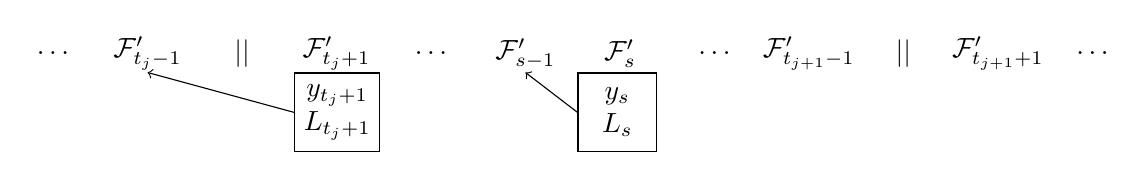
\begin{tikzpicture}[scale = 1.2]
    \tikzset{block/.style= {draw, rectangle, align=center,minimum width=1cm,minimum height=1cm},
            }
    %\draw[double] (0, 3 pt)node[above]{$\mathcal{F}_{t_j}$} -- (0,1/2 pt); 
    %\draw[double] (6, 3 pt)node[above]{$\mathcal{F}_{t_{j+1}-1}$} -- (6,1/2 pt); 
    \draw ; \node[] at (-1,-0.15) {$\ldots$};
    \draw ; \node[] at (0,-0.15) {$\mathcal{F}'_{t_j-1}$};
    \draw ; \node[] at (1,-0.15) {$||$};
    \draw ; \node[] at (2,-0.15) {$\mathcal{F}'_{t_j+1}$};
    \draw ; \node[] at (3,-0.15) {$\ldots$};
    \draw ; \node[] at (4,-0.15) {$\mathcal{F}'_{s-1}$};
    \draw ; \node[] at (5,-0.15) {$\mathcal{F}'_{s}$};
    \draw ; \node[] at (6,-0.15) {$\ldots$};
    \draw ; \node[] at (7,-0.15) {$\mathcal{F}'_{t_{j+1}-1}$};
    \draw ; \node[] at (8,-0.15) {$||$};
    \draw ; \node[] at (9,-0.15) {$\mathcal{F}'_{t_{j+1}+1}$};
    \draw ; \node[] at (10,-0.15) {$\ldots$};
    
    \draw[->] (1.55, -22 pt)node[block,right]{$y_{t_j+1}$\\$L_{t_j+1}$} -- (0,-10pt); 
    \draw[->] (4.55, -22 pt)node[block,right]{$y_{s}$\\$L_{s}$} -- (4,-10pt); 
    \end{tikzpicture}
    \caption{Filtration and  measurability of $(y_s)$ and $(L_s)$.}
    \label{fig:app_e}
\end{figure}

Yet simple but important observation is that for $\mathcal{J}_k=\{n_i:n_1<n_2<...<n_{\frac{k(k+1)}{2}}\}$ 
both stochastic processes $(L_{n_s})$, $(y_{n_s})$ are $\mathcal{F}'_{n_{s-1}}$-measurable and $(\psi_{n_s})$ is $\mathcal{F}'_{n_s}$-measurable.

To proceed we first notice that
\[
{\lambda_{\min}} \bigg(\lambda I_d+ \sum_{s=1}^{t_{k+1}-1} z_s z_s^\top\bigg) \succeq    {\lambda_{\min}} \bigg(\lambda I_d+\sum_{s \in\mathcal{J}_k} z_s z_s^\top\bigg).
\]
Invoking Lemma \ref{lem:preconditioner_expansion} with $\epsilon=\tilde\lambda=1$ and $\xi_s=L_s \psi_s$, it follows that
\begin{equation}\label{pe}
\begin{split}
&\sum_{s \in\mathcal{J}_k} z_s z_s^{\top}\quad\succeq\\
& \sum_{s\ \in\mathcal{J}_k}  (L_s\psi_s)(L_s\psi_s)^{\top} - \underbrace{\bigg[\sum_{s \in\mathcal{J}_k}  y_s (L_s \psi_s)^{\top}\bigg]^{\top}\bigg [ I_d+\sum_{s \in\mathcal{J}_k} y_sy_s^{\top}\bigg ]^{-1} \bigg [\sum_{s \in\mathcal{J}_k}  y_s (L_s \psi_s)^{\top}\bigg ]}_{(*)} -  I_d.
\end{split}
\end{equation}
Our goal is to find a lower bound of \eqref{pe}. To begin with, define $
\psi_{1,s} = 
\begin{bmatrix}
    w_{s-1}\\
    0
\end{bmatrix}$ and $
\psi_{2,s} = 
\begin{bmatrix}
    0\\
    \nu_{s}
\end{bmatrix}$ for $s\geq 1$ setting $w_0=0$ for simplicity. Noting that $L_s\psi_s = L_s\psi_{1,s} + \psi_{2,s}$, we apply Lemma \ref{lem:preconditioner_expansion} with $\epsilon=\frac{1}{2}$, $\tilde\lambda=1$ to obtain
\begin{equation}\label{pe_aux}
\begin{split}
    &\sum_{s \in\mathcal{J}_k}  (L_s\psi_{s})(L_s\psi_{s})^{\top}
    =\sum_{s \in\mathcal{J}_k}  (L_s\psi_{1,s})(L_s\psi_{1,s})^{\top} + \frac{1}{2}\sum_{s \in\mathcal{J}_k} \psi_{2,s}\psi_{2,s}^{\top}\\
    & - 2\underbrace{\bigg [\sum_{s \in\mathcal{J}_k}  \psi_{2,s} (L_s \psi_{1,s})^{\top}\bigg]^{\top}\bigg[ I_d+\sum_{s \in\mathcal{J}_k} \psi_{2,s}\psi_{2,s}^{\top}\bigg]^{-1}\bigg[\sum_{s \in\mathcal{J}_k}  \psi_{2,s} (L_s \psi_{1,s})^{\top}\bigg]}_{(**)} - \frac{1}{2} I_d.
\end{split}
\end{equation}
The first term of \eqref{pe_aux} is written as
\begin{align*}
    \sum_{s \in\mathcal{J}_k}  (L_s\psi_{1,s})(L_s\psi_{1,s})^{\top} & = \sum_{s \in\mathcal{J}_k}
    \begin{bmatrix}
        w_{s-1} w_{s-1}^{\top} & w_{s-1}(K_{v(s)}w_{s-1})^{\top}\\
        (K_{v(s)}w_{s-1}) w_{s-1}^{\top} & (K_{v(s)}w_{s-1})(K_{v(s)}w_{s-1})^{\top}     
    \end{bmatrix}
    \\
    & =: 
    \begin{bmatrix}
        X^{\top}X & X^{\top}Y\\
        Y^{\top}X & Y^{\top}Y
    \end{bmatrix},
\end{align*}
where $v(s)$ is indicates the episode number such that $s \in \mathcal{I}_{v(s)}$. By Lemma \ref{lem:tall_matrix}, we conclude that
\begin{align}\label{bar-lambda}
    \sum_{s \in\mathcal{J}_k}  (L_s\psi_{1,s})(L_s\psi_{1,s})^{\top} 
     = 
    \begin{bmatrix}
        X^{\top}X & X^{\top}Y\\
        Y^{\top}X & Y^{\top}Y
    \end{bmatrix}
     \succeq 
    \begin{bmatrix}
        \frac{\bar\lambda}{|Y|^2+\bar\lambda}X^{\top}X & 0\\
        0 & -\bar\lambda I_{n_u}
    \end{bmatrix}
\end{align}
for any $\bar\lambda>0$, where $X = [w_{n_1-1}, \cdots, w_{n_{k(k+1)/2}-1}]^{\top}$ and $Y = [K_{\nu(n_1)}w_{n_1-1}, \cdots, K_{\nu(n_{k(k+1)/2})}w_{n_{k(k+1)/2}-1}]^{\top}$.

Next, we invoke Lemma \ref{lem:noise_tail_bound} with $\epsilon=\frac{1}{2}\lambda_{\min}(\mathbf{W})$ for $\psi_s = w_{s-1}$, $\psi_s = \nu_{s}$ respectively to characterize good noise sets. 
Choosing $\rho = \log \frac{2}{\delta}$ in Lemma \ref{lem:noise_tail_bound}, there exists $C>0$ such that for any $\delta>0$ and $k\geq C \sqrt{\log (\frac{2}{\delta}) +d\log 9}$, the following events hold with probability at least $1-\delta$:
\begin{align*}
E_{1,k} &= \bigg\{w \in \Omega : \frac{1}{4}\lambda_{\min}(\mathbf{W}) k(k+1) I_{n} \preceq \sum_{s \in\mathcal{J}_k}  w_{s-1} w_{s-1}^{\top} \preceq \frac{1}{2}(\lambda_{\max}(\mathbf{W}) +\frac{1}{2}\lambda_{\min}(\mathbf{W})) k(k+1) I_{n}\bigg\},\\
E_{2,k} &= \bigg\{\nu \in \Omega_{\nu} : \frac{1}{2}\lambda_{\min}(\mathbf{W})k  I_{n_u} \preceq \sum_{s \in\mathcal{J}_k}  \nu_{s} \nu_{s}^{\top} \preceq (\lambda_{\max}(\mathbf{W}) +\frac{1}{2}\lambda_{\min}(\mathbf{W}))k I_{n_u} \bigg\}.
\end{align*}
Furthermore, from the observation,
\begin{equation*}
\begin{split}
\mathrm{tr}\bigg(\sum_{s \in\mathcal{J}_k} (K_{v(s)} w_{s-1}) (K_{v(s)}w_{s-1})^\top\bigg) &\leq \sum_{s \in\mathcal{J}_k} \mathrm{tr} ((K_{v(s)} w_{s-1}) (K_{v(s)}w_{s-1})^\top)\\
&\leq M_K^2 \sum_{s \in\mathcal{J}_k} |w_{s-1}|^2 \\
&= M_K^2 \mathrm{tr}\bigg(\sum_{s \in\mathcal{J}_k} w_{s-1}w_{s-1}^\top\bigg),
\end{split}
\end{equation*}
we also have the following event {whose subevent is $E_{1,k}$}:
\[E_{3,k} =\bigg \{w \in \Omega :  \sum_{s \in\mathcal{J}_k}  (K_{v(s)} w_{s-1})(K_{v(s)} w_{s-1})^{\top} \preceq \frac{n M_K^2}{2}(\lambda_{\max}(\mathbf{W}) +\frac{1}{2}\lambda_{\min}(\mathbf{W})) k(k+1) I_{n_u}\bigg\}.\]

where $\Omega_\nu \subset \Omega$ denotes the probability space associated with the random sequence $(\nu_s)_{s\geq 1}$ and $\Omega$ is the probability space representing all randomness in the algorithm as defined in the previous subsection. 

To proceed we choose $\bar{\lambda} = \frac{1}{8}\lambda_{\min}(\mathbf{W})k$ in \eqref{bar-lambda} and recall that $|Y|^2 = \lambda _{\max} (Y^\top Y)$. On the event $E_{1,k} \cap E_{2,k} \cap E_{3,k}$, first two terms on the right-hand side of \eqref{pe_aux} is lower bounded as
\begin{align*}
    &\sum_{s \in\mathcal{J}_k}  (L_s\psi_{1,s})(L_s\psi_{1,s})^{\top}+\frac{1}{2}\sum_{s \in\mathcal{J}_k}  \psi_{2,s}\psi_{2,s}^{\top}\\
    &\succeq
    \begin{bmatrix}
    \frac{\bar\lambda}{|Y|^2+\bar\lambda}X^{\top}X & 0\\
    0 & -\bar\lambda I_{n_u}
    \end{bmatrix} + \frac{1}{2}
   \sum_{s\in\mathcal{J}_k} 
   \begin{bmatrix}0 \\ \nu_s  
   \end{bmatrix}
    \begin{bmatrix}
        0 &\nu_s^\top
    \end{bmatrix}\\
    &\succeq
    \begin{bmatrix}
    \frac{\frac{1}{32}\lambda_{\min}^2(\mathbf{W})k^2(k-1)}{\frac{nM_K^2}{2}(\lambda_{\max}(\mathbf{W})+\frac{1}{2}\lambda_{\min}(\mathbf{W}))k(k-1)+\frac{1}{8}\lambda_{\min}(\mathbf{W})} I_{n} &0\\ 
        0 & -\frac{1}{8}\lambda_{\min}(\mathbf{W}) k I_{n_u}
    \end{bmatrix}
    +
    \begin{bmatrix}
        0 & 0\\
        0 & \frac{1}{4}\lambda_{\min}(\mathbf{W})kI_{n_u}
    \end{bmatrix}
    \\
    &= 
    k\begin{bmatrix}
    \frac{\lambda_{\min}^2(\mathbf{W})k(k-1)}{16nM_K^2(\lambda_{\max}(\mathbf{W})+\frac{1}{2}\lambda_{\min}(\mathbf{W}))k(k-1)+4\lambda_{\min}(\mathbf{W})} I_{n}&0\\ 
        0 & \frac{1}{8}\lambda_{\min}(\mathbf{W})I_{n_u}
    \end{bmatrix}
    \\
    &\succeq C k I_{d}
\end{align*}
for some $C>0$. 

We next deal with $(*)$ in \eqref{pe} and $(**)$ in \eqref{pe_aux} together as they have the same  structure. Let us begin by defining 
\[
S_k(\psi_{2},L\psi_{1}) := \bigg[\sum_{s \in\mathcal{J}_k}  \psi_{2,s} (L_s \psi_{1,s})^{\top}\bigg]^{\top}\bigg[I_d+\sum_{s \in\mathcal{J}_k} \psi_{2,s}\psi_{2,s}^{\top}\bigg]^{-1}\bigg[\sum_{s \in\mathcal{J}_k}  \psi_{2,s} (L_s \psi_{1,s})^{\top}\bigg].
\]
Similarly,
\[
S_k(y,L\psi) := \bigg[\sum_{s \in\mathcal{J}_k}  y_s (L_s \psi_{s})^{\top}\bigg]^{\top}\bigg[I_d+\sum_{s \in\mathcal{J}_k} y_s y_s^{\top}\bigg]^{-1}\bigg[\sum_{s \in\mathcal{J}_k}  y_s (L_s \psi_{s})^{\top}\bigg].
\]

Applying Lemma \ref{lem:self-normalized_matrix} with $\rho=\log(\frac{1}{\delta})$ to the stochastic processes $(\psi_s)_{s\in \mathcal{J}_k}$ and $(y_s)_{s\in \mathcal{J}_k}$, each of the following events holds with probability at least $1-\delta$:
\begin{align*}
E_{4,k} &=\bigg \{w \in \Omega, \nu \in \Omega_{\nu}:|S_k(\psi_{2},L\psi_{1})|\leq 7\bar L_{\nu}^2
(M_K^2+2)\log\bigg(\frac{e^d \det(I_d+\sum_{s \in\mathcal{J}_k}\psi_{2,s}\psi_{2,s}^{\top})}{\delta}\bigg)\bigg\},\\
E_{5,k} &=\bigg \{w \in \Omega, \nu \in \Omega_{\nu}:|S_k(y,L\psi)|\leq 7\bar L^2(M_K^2+2)\log\bigg(\frac{e^d \det(I_d+\sum_{s \in\mathcal{J}_k} y_s y_s^{\top})}{\delta}\bigg)\bigg\},
\end{align*}
since $\max_{s \leq t} |L_s| \leq \sqrt{M_K^2+2}$ 
with $L_s := 
\begin{bmatrix}
    I_n & 0\\
    K_j & I_{n_u}
\end{bmatrix}.$ To verify, we recall that $|L_s| = \sqrt{\lambda_{\max}(L_sL_s^{\top})}$. Here,
\[
L_sL_s^{\top} =
\begin{bmatrix}
    I_{n} &K_j^{\top}\\ 
        K_j & K_jK_j^{\top}+I_{n_u}
    \end{bmatrix}.
\]
Fixing $v=\begin{bmatrix}x^{\top} & y^{\top}\end{bmatrix}^{\top}$ such that $|v|=1$ where $x\in\mathbb{R}^n$ and  $y\in\mathbb{R}^{n_u}$, we have
\begin{align*}
    v^{\top}
    \begin{bmatrix}
    I_{n} &K_j^{\top}\\ 
        K_j & K_jK_j^{\top}+I_{n_u}
    \end{bmatrix}
    v
    &\leq  
    |x|^2+2x^{\top}K_j^{\top}y + M_K^2|y|^2 + |y|^2\\
    &\leq (M_K^2+1)(x^2+y^2)+|y|^2\\
    &\leq M_K^2+2.
\end{align*}
\begin{itemize}
\item Bound of $S_k(\psi_2,L\psi_1)$ on $E_{2,k}\cap E_{4,k}$:

On $E_{2,k}$,
\begin{align*}
\det\bigg(I_d+\sum_{s \in\mathcal{J}_k}\psi_{2,s}\psi_{2,s}^{\top}\bigg)^{\frac{1}{d}} &\leq \frac{1}{d}(d+\sum_{s \in\mathcal{J}_k}\psi_{2,s}^{\top}\psi_{2,s})\\
& = \frac{1}{d}(d+\sum_{s \in\mathcal{J}_k}|\nu_{s}|^2)\\
& \leq \frac{n_u}{d}(\lambda_{\max}(\mathbf{W}) +\frac{1}{2}\lambda_{\min}(\mathbf{W}))k+1\\
& \leq C k
\end{align*}
for some $C>0$ where the second inequality follows by
\begin{align*}
\sum_{s\in\mathcal{J}} |\nu_s|^2 =\mathrm{tr}(\sum_{s\in\mathcal{J}_k} \nu_s \nu_s ^\top) &\leq n_u \lambda_{\max}({\sum_{s\in\mathcal{J}_k} \nu_s\nu_s^\top})\\
& \leq n_u(\lambda_{\max}(\mathbf{W}) +\frac{1}{2}\lambda_{\min}(\mathbf{W}))k.
\end{align*}


Altogether, on the event $E_{2,k}\cap E_{4,k}$,
\begin{equation*}
\begin{split}
S_k(\psi_{2},L\psi_{1})&=\bigg|\bigg[\sum_{s \in\mathcal{J}_k} \psi_{2,s} (L_s \psi_{1,s})^{\top}\bigg]^{\top}\bigg[I_d+\sum_{s \in\mathcal{J}_k}\psi_{2,s}\psi_{2,s}^{\top}\bigg]^{-1}\bigg[\sum_{s \in\mathcal{J}_k} \psi_{2,s} (L_s \psi_{1,s})^{\top}\bigg]\bigg|\\
&\leq 7\bar L_{\nu}^2(M_K^2+2)\log\bigg(\frac{Ce^d k^d}{\delta}\bigg).
\end{split}
\end{equation*}

\item Bound of $S_k(y,L\psi)$ on $F_{t_{k+1}} \cap E_{1,k} \cap E_{5,k}$: 

On $E_{1,k}$, 
\begin{align*}
&\det\bigg(I_d+\sum_{s \in\mathcal{J}_k} y_s y_s^{\top}\bigg)^{\frac{1}{d}} \\
&\leq \frac{1}{d}\bigg(d+\sum_{s \in\mathcal{J}_k}|y_s|^2\bigg)\\
& = \frac{1}{d}\bigg(d+\sum_{s \in\mathcal{J}_k}(\underbrace{|x_s-w_{s-1}|^2}_{\leq 2|x_s|^2+2|w_{s-1}|^2}+\underbrace{|K_{v(s)}(x_s-w_{s-1})|^2}_{\leq 2M_K^2|x_s|^2+2M_K^2|w_{s-1}|^2})\bigg)\\
& \leq \frac{1}{d}\bigg(d+\sum_{s \in\mathcal{J}_k}((2+2M_K^2)|x_s|^2+(2+2M_K^2)|w_{s-1}|^2)\bigg)\\
& \leq  \frac{(M_K^2+1)}{d}\bigg(\underbrace{2\sum_{s \in\mathcal{J}_k}|x_s|^2}_\text{(a)}+ \underbrace{n(\lambda_{\max}(\mathbf{W}) +\frac{1}{2}\lambda_{\min}(\mathbf{W}))k(k-1)}_\text{by taking trace in $E_{1,k}$}\bigg)+1,
\end{align*}
where the last inequality follows from
\begin{align*}
\sum_{s\in\mathcal{J}} |w_{s-1}|^2 =\mathrm{tr}\bigg(\sum_{s\in\mathcal{J}_k} w_{s-1} w_{s-1} ^\top\bigg) &\leq n \lambda_{\max}\bigg({\sum_{s\in\mathcal{J}_k} w_{s-1}w_{s-1}^\top}\bigg)\\
& \leq \frac{n}{2}\bigg(\lambda_{\max}(\mathbf{W}) +\frac{1}{2}\lambda_{\min}(\mathbf{W})\bigg)k(k-1).
\end{align*}

To bound (a) above, let us observe that $t_{k+1}=\frac{(k+1)(k+2)}{2} \leq k^p$ for any $p\geq 3$ and consider the event $F_{t_{k+1}} \cap E_{1,k}$. Applying Lemma~\ref{lem:state_log} with $\delta=k^{-p} \leq t_{k+1}^{-1}$, we deduce that
\begin{align*}
   \sum_{s\in\mathcal{J}_k} |x_s|^2=\sum_{s\in\mathcal{J}_k}|x_s|^2 & \leq t_{k+1} \max_{s \leq t_{k+1}}|x_s|^2\\
   &\leq t_{k+1} \bigg( C(\log k)^3 \sqrt{\log k} \bigg)^{2(d+1)}\\
   &\leq C k^2\bigg( k\sqrt{\log k}\bigg)^{2(d+1)}\\
   & \leq C k^{3d+5}
\end{align*}
for some $C>0$ depending on $p\geq 3$ and the constant from Lemma~\ref{lem:state_log}.

Therefore, on the event $F_{t_{k+1}} \cap E_{1,k}\cap E_{5,k}$, we have
\begin{align*}
    \det\bigg(I_d+\sum_{s\in\mathcal{J}_k} y_s y_s^{\top}\bigg)^{\frac{1}{d}}&\leq (M_K^2+1)\bigg(\frac{2C}{d}k^{3d+5}+ \bigg(\lambda_{\max}(\mathbf{W}) +\frac{1}{2}\lambda_{\min}(\mathbf{W})\bigg)k(k-1)\bigg)+1\\
    &\leq C k^{3d+5}
\end{align*}
for some constant $C>0$. As a result,
\begin{equation*}
\begin{split}
S_k(y,L\psi)&=\bigg|\bigg[\sum_{s\in\mathcal{J}_k} y_s (L_s \psi_{s})^{\top}\bigg]^{\top}\bigg[I_d+\sum_{s\in\mathcal{J}_k}y_sy_s^{\top}\bigg]^{-1}\bigg[\sum_{s\in\mathcal{J}_k} y_s (L_s \psi_{s})^{\top}\bigg]\bigg|\\
&\leq 7\bar L^2(M_K^2+2)\log\bigg(\frac{Ce^d k^{d(3d+5)}}{\delta}\bigg).
\end{split}
\end{equation*}


\end{itemize}

Combining altogether and plugging them into \eqref{pe}, on the event $F_{t_{k+1}} \cap E_{1,k} \cap E_{2,k}\cap E_{3,k}\cap E_{4,k}\cap E_{5,k}$, one can derive that
\begin{equation*}
\begin{split}
    \lambda_{\min}(\lambda I_d + \sum_{s\in \mathcal{J}_k} z_s z_s^{\top}) 
    &\geq  \lambda+ C_1 k - C_2\log k  + C_3 \log(\delta)-C_4\\
    & \geq C k
\end{split}
\end{equation*}
for some $C_i,C>0$ with $\delta=k^{-p}$ and $k \geq k_0$ for $k_0$ large enough. In turn, we have the concentration bound for the excitation yielding that 
\begin{align*}
    &Pr\bigg(\lambda_{\min}(\lambda I_d + \sum_{s=1}^{t_{k+1}-1} z_s z_s^{\top}) \geq C k\bigg)\\
    & \geq 1-Pr(F^c_{t_{k+1}} \cup E^c_{1,k} \cup E^c_{2,k}\cup E^c_{3,k}\cup E^c_{4,k}\cup E^c_{5,k})\\
    & \geq 1-9\delta.
\end{align*}
Finally, defining the event $\bar{F}_{k+1}:=F_{t_{k+1}}\cap E_{1,k} \cap E_{2,k}\cap E_{3,k}\cap E_{4,k}\cap E_{5,k}$,
\begin{align*}
    \mathbb{E}\bigg[\frac{1}{\lambda^p_{\min,k+1}}\bigg] 
    &= \mathbb{E}\bigg[\frac{1}{\lambda^p_{\min,k+1}}\mathbbm{1}_{\bar{F}_{k+1}}\bigg] + \mathbb{E}\bigg[\frac{1}{\lambda^p_{\min,k+1}}\mathbbm{1}_{\bar{F}_{k+1}^c}\bigg]\nonumber\\
    &\leq C\mathbb{E}\bigg[ k^{-p}\mathbbm{1}_{\bar{F}_{k+1}}\bigg] + \mathbb{E}\bigg[\mathbbm{1}_{\bar{F}_{k+1}^c}\bigg]\nonumber\\
    &\leq C k^{-p} + 9\delta \leq C k^{-p},
\end{align*}
where second inequality holds from $\lambda_{\min,t} \geq \lambda \geq 1$. 
\end{proof}

\subsection{Proof of Theorem~\ref{thm:exact_appox}}
\label{app:thm:exact_appox}
\begin{proof}
It follows from \eqref{half_1} in Proposition \ref{prop:half_exact_true}  that 
\[
\mathbb{E}_{\theta_t \sim \mu_{t}}[|\theta_t-\theta_*|^p_{P_{t}}|h_{t}]\leq (2p)^p\bigg(\frac{4}{m^2}|P_{t}^{-\frac{1}{2}}\nabla_{\theta} U'_{t}(\theta_*)|^2 + \frac{4dn}{m}+ 64m+C\bigg)^{\frac{p}{2}},
\]
where $U_t'(\theta) =\sum_{s=1}^{t-1}\log p_w(x_{s+1}-\Theta^{\top}z_s)$.
Recalling $\lambda_{\min,t}=\lambda_{\min,t}(P_t)$, it follows that
\[
\lambda^{\frac{p}{2}}_{\min,t}\mathbb{E}[|\theta_t -\theta_*|^p]\leq  \mathbb{E}[|\theta_t-\theta_*|^p_{P_{t}}],
\] and hence,
\begin{align}\label{fe}
    &\mathbb{E}[\mathbb{E}_{\theta_t \sim \mu_t}[|\theta_t-\theta_*|^p|h_{t}]] \nonumber \\
    & \leq (2p)^p \sqrt{\mathbb{E}\bigg[\frac{1}{\lambda_{\min,t}^{p}}\bigg]}\sqrt{\mathbb{E}\bigg[\bigg(\frac{4}{m^2}|P_{t}^{-\frac{1}{2}}\nabla_{\theta} U'_{t}(\theta_*)|^2+  \frac{4dn}{m}+ 64m+C\bigg)^p\bigg]}\nonumber\\
    & \leq (2p)^p \sqrt{\mathbb{E}\bigg[\frac{1}{\lambda_{\min,t}^{p}}\bigg]}\sqrt{2^{p-1}\bigg(\frac{4^p}{m^{2p}}\mathbb{E}\bigg[|P_{t}^{-\frac{1}{2}}\nabla_{\theta} U'_{t}(\theta_*)|^{2p}\bigg] + \bigg( \frac{4dn}{m}+ 64m+C\bigg)^p\bigg)},
\end{align}
where the second inequality holds by Jensen's inequality and the outer expectation is taken with respect to the history at time $t$.

To bound $\mathbb{E}\bigg[|P_{t}^{-\frac{1}{2}}\nabla_{\theta} U'_{t}(\theta_*)|^{2p}\bigg]$, let us first define $Z:=\begin{bmatrix} z_1& \cdots &z_{t-1} \end{bmatrix}^\top$ and denote the $j$th component of noise $w_t$ by $w_t(j)$. A naive bound is achieved as
\begin{align}\label{navie:bd}
    |P_{t}^{-\frac{1}{2}}\nabla_{\theta} U'_{t}(\theta_*)|^{2}&= \sum_{j=1}^{n}\sum_{s',s=1}^{t-1}\frac{\partial \log p_w(w_{s'})}{\partial w_{s'}(j)}(Z(Z^{\top}Z + \lambda I_d)^{-1}Z^{\top})_{s's}\frac{\partial \log p_w(w_s)}{\partial w_s(j)}\notag\\
    &\leq \sum_{j=1}^{n}\sum_{s',s=1}^{t-1}\frac{\partial \log p_w(w_{s'})}{\partial w_{s'}(j)}(Z(Z^{\top}Z)^{-1}Z^{\top})_{s's}\frac{\partial \log p_w(w_s)}{\partial w_s(j)}\notag\\
    &\leq \sum_{j=1}^{n}\sum_{s=1}^{t-1}\bigg(\frac{\partial \log p_w(w_s)}{\partial w_s(j)}\bigg)^2 \notag\\
    &= \sum_{s=1}^{t-1}|\nabla_w \log p_w(w_s)|^2,
\end{align}
where the second inequality follows from the fact that $Z(Z^{\top}Z)^{-1}Z^{\top}$ is a projection matrix.

We now claim that $\mathbb{E}\bigg[|P_{t}^{-\frac{1}{2}}\nabla_{\theta} U'_{t}(\theta_*)|^{2p}\bigg]$ has a better bound compared to the naive one with high probability leveraging self-normalized bound for vector-valued martingale. For $s\geq 0$, let us consider the natural filtration 
\[
\mathcal{F}_s = \sigma((z_1,...,z_{s+1})),
\]
where $z_s=(x_s,u_s)$. Clearly, for $s\geq 1$, $z_s$ is $\mathcal{F}_{s-1}$-measurable and the random vector $\nabla_w \log p_w(w_s)$ is $\mathcal{F}_s$-measurable. Then for each $j \in [1,n]$, we set $\eta_s=\frac{\partial\log p_w(w_{s})}{\partial w_{s}(j)}$, $X_s=z_s$, $S_t=\sum_{s=1}^{t-1} \eta_s X_s=\sum_{s=1}^{t-1}\frac{\partial\log p_w(w_{s})}{\partial w_{s}(j)}z_s$. Here, $\eta_s$ is a $\frac{M}{\sqrt{m}}$-sub-Gaussian random variable since $v^\top \nabla_w \log p_w (w_t)$ is $\frac{M}{\sqrt{m}}$-sub-Gaussian random variable for any $v\in\mathbb{R}^n$ given when $w_t$ is sub-Gaussian (Proposition 2.18 in \cite{ledoux2001concentration}). Together with the fact that
\[
\lambda I_d + \sum_{s=1}^{t-1} X_s X_s^\top = \lambda I_d+Z^\top Z,
\]
and the result for self-normalized bound~\ref{lem:self_norm},
\begin{align*}
    &(\sum _{s=1}^{t-1} \eta_s X_s)^\top(\lambda I_d + \sum_{s=1}^{t-1} X_s X_s^\top)^{-1}(\sum _{s=1}^{t-1} \eta_s X_s)\\
    &=\sum_{s,s'=1}^{t-1}\frac{\partial \log p_w(w_{s'})}{\partial w_{s'}(j)}(Z(Z^{\top}Z + \lambda I_d)^{-1}Z^{\top})_{s's}\frac{\partial \log p_w(w_s)}{\partial w_s(j)}\notag\\
    &\leq 2\frac{M^2}{m}\log\bigg(\frac{n}{\delta}\bigg(\frac{\sqrt[n]{\det(P_{t})}}{\det(\lambda I_d)}\bigg)^{\frac{1}{2}}\bigg),
\end{align*}
holds with probability at least $1-\frac{\delta}{n}$.
Here, we use the fact that $\det (\lambda I_d+Z^\top Z) =\sqrt[n]{\det(\lambda I_{dn}+\sum_{s=1}^{t-1} \mathrm{blkdiag}\{z_s z_s^\top\}_{i=1}^n)}  =\sqrt[n]{\det(P_{t})}$.

By the union bound argument,
\begin{align}\label{tight:bd}
    |P_{t}^{-\frac{1}{2}}\nabla_{\theta} U'_{t}(\theta_*)|^{2} &= \sum_{j=1}^n\sum_{s,s'=1}^{t-1}\frac{\partial \log p_w(w_{s'})}{\partial w_{s'}(j)}(Z(Z^{\top}Z + \lambda I_d)^{-1}Z^{\top})_{s's}\frac{\partial \log p_w(w_s)}{\partial w_s(j)}\notag\\ 
    &\leq 2\frac{nM^2}{m}\log\bigg(\frac{n}{\delta}\bigg(\frac{\sqrt[n]{\det(P_{t})}}{\det(\lambda I_d)}\bigg)^{\frac{1}{2}}\bigg),
\end{align}
with probability at least $1- \delta$ for any $\delta>0$. Let us denote this event as $\tilde E$ so that $Pr(\tilde E) \geq 1-\delta$.

Combining the naive bound~\eqref{navie:bd} and improved bound~\eqref{tight:bd}, 
\begin{align}\label{se}
      &\mathbb{E}\bigg[|P_{t}^{-\frac{1}{2}}\nabla_{\theta} U'_{t}(\theta_*)|^{2p}\bigg]\nonumber\\ &=\mathbb{E}\bigg[\mathbbm{1}_{\tilde E}|P_{t}^{-\frac{1}{2}}\nabla_{\theta} U'_{t}(\theta_*)|^{2p}\bigg] + \mathbb{E}\bigg[\mathbbm{1}_{\tilde E^c}|P_{t}^{-\frac{1}{2}}\nabla_{\theta} U'_{t}(\theta_*)|^{2p}\bigg]\nonumber\\
      &\leq \underbrace{\mathbb{E}\bigg[\bigg(2\frac{nM^2}{m}\log\bigg(\frac{n}{\delta}\bigg(\frac{\sqrt[n]{\det(P_{t})}}{\det(\lambda I_d)}\bigg)^{\frac{1}{2}}\bigg)\bigg)^p\bigg]}_\text{by \eqref{tight:bd}} + \sqrt{\mathbb{E}\bigg[\mathbbm{1}_{\tilde E^c}\bigg]}\sqrt{\mathbb{E}\bigg[|P_{t}^{-\frac{1}{2}}\nabla_{\theta} U'_{t}(\theta_*)|^{4p}\bigg]}\nonumber\\
      &\leq \mathbb{E}\bigg[\bigg(2\frac{nM^2}{m}\log\bigg(\frac{n}{\delta}\bigg(\frac{\lambda_{\max,t}}{\lambda}\bigg)^{\frac{d}{2}}\bigg)\bigg)^p\bigg]+\sqrt{\delta}\underbrace{\sqrt{\mathbb{E}\bigg[\bigg(\sum_{s=1}^{t-1}|\nabla_w \log p_w(w_s)|^2\bigg)^{2p}\bigg]}}_\text{by \eqref{navie:bd}}.
\end{align}
We handle two terms on the right hand side separately. Recall that $g:x\rightarrow (\log x)^p$ is concave on $x\geq 1$ whenever $p >0$. By Jensen's inequality, the first term is bounded as
\begin{equation*}
\begin{split}
    \mathbb{E}\bigg[\bigg(2\frac{nM^2}{m}\log\bigg(\frac{n}{\delta}\bigg(\frac{\lambda_{\max,t}}{\lambda}\bigg)^{\frac{d}{2}}\bigg)\bigg)^p\bigg]&=\mathbb{E}\bigg[\bigg(\frac{dnM^2}{m}\log\bigg(\frac{n}{\delta^{\frac{2}{d}}}\frac{\lambda_{\max,t}}{\lambda}\bigg)\bigg)^p\bigg]\\
    &\leq \bigg(\frac{dnM^2}{m}\bigg)^p\log\bigg(\frac{n}{\lambda\delta^{\frac{2}{d}}}\mathbb{E}[\lambda_{\max,t}]\bigg)^p\\
    &\leq \bigg(\frac{dnM^2}{m}\bigg)^p\log\bigg(\frac{n}{\lambda\delta^{\frac{2}{d}}}\mathbb{E}[\frac{1}{n}\mathrm{tr}(P_{t})]\bigg)^p\\
    &\leq \bigg(\frac{dnM^2}{m}\bigg)^p\log\bigg(\frac{n}{\lambda\delta^{\frac{2}{d}}}\mathbb{E}[d\lambda + \sum_{s=1}^{t-1}|z_s|^2]\bigg)^p\\
    &\leq \bigg(\frac{dnM^2}{m}\bigg)^p\log\bigg(\frac{n}{\lambda\delta^{\frac{2}{d}}}\bigg(d\lambda+M_K^2t\mathbb{E}[\max_{j\leq t-1}|x_j|^2]\bigg)\bigg)^p\\
    &\leq \bigg(\frac{dnM^2}{m}\bigg)^p\log\bigg(\frac{n}{\lambda\delta^{\frac{2}{d}}}\bigg(d\lambda+CM_K^2{t}^{7d+8}\bigg)\bigg)^p, 
\end{split}
\end{equation*}
where the last inequality holds from the Theorem~\ref{thm:state_poly}.

On the other hand, the second term of \eqref{se} can be handled similarly. Recalling Jensen's inequality,
\[
\bigg(\frac{\sum_{i}^n a_i}{n}\bigg )^{2p} \leq \frac{\sum_{i=1}^n a_i^{2p}}{n}
\]
for $a_i \in \mathbb{R}$ and $p \geq 1$, we have that
\begin{equation*}
\begin{split}
\sqrt{\delta}\sqrt{\mathbb{E}\bigg[\bigg(\sum_{s=1}^{t-1}|\nabla_w \log p_w(w_s)|^2\bigg)^{2p}\bigg]}&\leq \sqrt{\delta}\sqrt{t^{2p-1}\mathbb{E}\bigg[\sum_{s=1}^{t-1}|\nabla_w \log p_w(w_s)|^{4p}\bigg]}\\
&\leq \sqrt{\delta}t^{p}\sqrt{\mathbb{E}\bigg[|\nabla_w \log p_w(w_t)|^{4p}\bigg]}\\
&\leq \sqrt{\delta}t^{p}\sqrt{\bigg(\frac{4M^2}{m}\bigg)^{2p}(2p)!}\\
&\leq 8^p\frac{M^{2p}}{m^{p}}p^p\sqrt{\delta}t^{p},
\end{split}
\end{equation*}
where the third inequality comes from well-known fact that any $\bar L$-sub-Gaussian random vector $X$ satisfies $\E[X^{2q}] \leq q!(4{\bar L}^2)^q$ for any $q>0$.

Choosing $\delta = \frac{1}{t^{2p}}$ and combining two bounds,
\begin{align*}
    \mathbb{E}\bigg[|P_{t}^{-\frac{1}{2}}\nabla_{\theta} U'_{t}(\theta_*)|^{2p}\bigg]&\leq  \bigg(\frac{dnM^2}{m}\bigg)^p\log\bigg(\frac{n}{\lambda\delta^{\frac{2}{d}}}\bigg(d\lambda+CM_K^2{t}^{7d+8}\bigg)\bigg)^p+8^p\frac{M^{2p}}{m^{p}}p^p\sqrt{\delta}t^{p}\\
    &\leq\bigg(\frac{dnM^2}{m}\bigg)^p\log\bigg(nt^{\frac{4p}{d}}\bigg(d+\frac{CM_K^2}{\lambda}t^{7d+8}\bigg)\bigg)^p+8^p\frac{M^{2p}}{m^{p}}p^p.
\end{align*}

Finally, going back to \eqref{fe},
\begin{equation*}
\begin{split}
    &\mathbb{E}[\mathbb{E}_{\theta_t \sim \mu_{t}}[|\theta_t-\theta_*|^p|h_{t}]] \\
    & \leq (2p)^p \sqrt{\mathbb{E}\bigg[\frac{1}{\lambda_{\min,t}^{p}}\bigg]}\sqrt{2^{p-1}\bigg(\frac{4^p}{m^{2p}}\mathbb{E}\bigg[|P_{t}^{-\frac{1}{2}}\nabla_{\theta} U'_{t}(\theta_*)|^{2p}\bigg] + \bigg( \frac{4dn}{m}+ 64m+C\bigg)^p\bigg)}\\
    &\leq (2p)^p \sqrt{\mathbb{E}\bigg[\frac{1}{\lambda_{\min,t}^{p}}\bigg]}\\
    &\quad\quad \times\sqrt{\frac{2^{3p-1}(dn)^pM^{2p}}{m^{3p}}\log\bigg(nt^{\frac{4p}{d}}\bigg(d+\frac{CM_K^2}{\lambda}t^{7d+8}\bigg)\bigg)^p+ \frac{2^{6p-1}}{m^{3p}}M^{2p}p^p+\bigg( \frac{4dn}{m}+ 64m+C\bigg)^p}\\
    &\leq \bigg((2p)^pC\sqrt{\frac{2^{3p-1}(dn)^pM^{2p}}{m^{3p}}\log\bigg(nt^{\frac{4p}{d}}\bigg(d+\frac{CM_K^2}{\lambda}t^{7d+8}\bigg)\bigg)^p+ \frac{2^{6p-1}}{m^{3p}}M^{2p}p^p+\bigg( \frac{4dn}{m}+ 64m+C\bigg)^p}\bigg)t^{-\frac{p}{4}},
\end{split}
\end{equation*}
where last inequality holds thanks to Proposition \ref{prop:pers-ex}.

For the concentration of the approximate posterior, we invoke Jensen's inequality to derive
\begin{equation}\nonumber
\begin{split}
    \mathbb{E}\bigg[\mathbb{E}_{\tilde{\theta}_t \sim \tilde{\mu}_t}\big[| \tilde{\theta}_t - \theta_* |^p | h_{t}\big ]\bigg] &= \mathbb{E}\bigg[\mathbb{E}_{\theta_t \sim \mu_t, \tilde{\theta}_t \sim \tilde{\mu}_t}\big[| \tilde{\theta}_t - \theta_* |^p\big | h_{t}]\bigg]\\
    &\leq 2^{p-1}\mathbb{E}\bigg[\mathbb{E}_{\theta_t \sim \mu_t, \tilde{\theta}_t \sim \tilde{\mu}_t}\big[| \theta_t- \tilde{\theta}_t |^p | h_{t} \big ]\bigg]+2^{p-1}\mathbb{E}\bigg[\mathbb{E}_{\theta_t \sim \mu_t, \tilde{\theta}_t \sim \tilde{\mu}_t}\big[| \theta_t - \theta_* |^p|h_{t} \big ]\bigg]\\
    &\leq 2^{p-1}\mathbb{E}\bigg[\frac{D_p}{(\sqrt{\lambda_{\min,t}})^p}\bigg]+2^{p-1}C\bigg(t^{-\frac{1}{4}}\sqrt{\log t}\bigg)^p\\
    &\leq C\bigg(t^{-\frac{1}{4}}\sqrt{\log t}\bigg)^p,
\end{split}
\end{equation}
where the second inequality comes from Proposition \ref{prop:ula} and the concentration result of exact posterior above.
\end{proof}



\subsection{Proof of Theorem~\ref{thm:improved}}
\label{app:thm:improved}
\begin{proof}
At $k$th episode, for timestep $t \in [t_k,t_{k+1})$, $x_{t}$ is written as
%\begin{equation}\label{state_norm}
%    x_t = (A_*+B_*K(\tilde{\theta}_k))^{t-t_k+1}x_{t_k-1} + \sum_{i=t_k}^t (A_*+B_*K(\tilde{\theta}_k))^{i-t_k}w_{i-1}.
%\end{equation}
\begin{equation}\label{state_norm}
    x_{t+1} = (A_*+B_*K(\tilde{\theta}_{t}))x_{t}+ r_t,
\end{equation}
where $r_t = B_*\nu_t +w_t$.
Squaring and taking expectations on both sides of the equation above with respect to noises, the prior and randomized actions,
\begin{equation}\label{sb2}
    \mathbb{E}[|x_{t+1}|^2] \leq \mathbb{E}[|D_{t}|^{2}|x_{t}|^2]+ \mathbb{E}[|r_{t}|^2],
\end{equation}
where $D_{t} = A_*+B_*K(\tilde{\theta}_{t})$.

Since $\theta_*$ is stabilizable, it is clear to see that there exists $\epsilon_0>0$ small for which $|\theta-\theta_*|\leq \epsilon_0$ implies that $|A_*+B_* K(\theta)|\leq \Delta<1$ for some $\Delta>0$. Splitting $\mathbb{E}[|D_t|^2|x_t|^2]$ around the true system parameter $\theta_*$,
\[
\mathbb{E}[|D_{t}|^2|x_{t}|^2] = \underbrace{\mathbb{E}[|D_{t}|^2|x_{t}|^2\mathbbm{1}_{|\tilde{\theta}_{t}-\theta_*| \leq \epsilon_0}]}_{(i)} +\underbrace{\mathbb{E}[|D_{t}|^2|x_{t}|^2\mathbbm{1}_{|\tilde{\theta}_{t}-\theta_*| > \epsilon_0}]}_{(ii)}. 
\]
One can see that (i) is bounded by $\Delta^2 \mathbb{E}[|x_{t}|^2]$ by the construction. For (ii), we note that $|D_{t}| \leq M_\rho$ by Assumption \ref{ass:init_bound}. Using Cauchy-Schwartz inequality, (ii) is bounded as
\begin{equation}\label{second_1}
\mathbb{E}[|D_{t}|^2|x_{t}|^2\mathbbm{1}_{|\tilde{\theta}_{t}-\theta_*| > \epsilon_0}]] \leq M_{\rho}^2\sqrt{Pr(|\tilde{\theta}_{t}-\theta_*|>\epsilon_0)}\sqrt{\mathbb{E}[|x_{t}|^4]}.
\end{equation}
By Markov's inequality,
\begin{align*}
    Pr(|\tilde{\theta}_{t}-\theta_*|>\epsilon_0) &\leq \frac{\mathbb{E}[|\tilde{\theta}_{t}-\theta_*|^p]}{\epsilon_0^p}\\
    &\leq C\bigg(t^{-\frac{1}{4}}\sqrt{\log t}\bigg)^p,
\end{align*}
where the last inequality holds for $t\geq t_0$ thanks to Theorem \ref{thm:exact_appox}, and $C$ is a positive constant depending only on $p$ and $\epsilon_0$. 
Taking $p$ large enough to satisfy $p>28(d+1)$, Theorem \ref{thm:state_poly} yields that 
\begin{align*}
M_{\rho}^2\sqrt{Pr(|\tilde{\theta}_{t}-\theta_*|>\epsilon_0)}\sqrt{\mathbb{E}[|x_{t}|^4]}
    &\leq M_{\rho}^2C \bigg(t^{-\frac{1}{4}}\sqrt{\log t}\bigg)^pt^{7(d+1)} <C
\end{align*}
for some $C>0$.

Therefore, $\mathbb{E}[|x_{t+1}|^2]$ is estimated as
\[
\mathbb{E}[|x_{t+1}|^2] \leq \Delta^2\mathbb{E}[|x_{t}|^2]+C+\mathbb{E}[|r_{t}|^2].
\]
As $r_t$ is sub-Gaussian, we also have $\mathbb{E}[|r_t|^2]$ is bounded, and hence, 
\[
\mathbb{E}[|x_{t}|^2] <C
\]
for all $t \in [1,T]$ and $C>0$ by the recursive relation.

To handle the fourth moment, we take the fourth power on both sides and expectation to \eqref{state_norm} to obtain
\begin{align*}
    &\mathbb{E}[|x_{t+1}|^4]\\
    &\leq \mathbb{E}[|D_{t}x_{t}|^4]+\underbrace{4\mathbb{E}[|D_{t}x_{t}|^2(D_{t}x_{t})^{\top}w_{t}]}_{=0}+6\mathbb{E}[|D_{t}x_{t}|^2|r_{t}|^2] +4\mathbb{E}[|D_{t}x_{t}||r_{t}|^3] + \mathbb{E}[|r_t|^4]\\
    &\leq [|D_{t}|^4|x_{t}|^4\mathbbm{1}_{|\tilde{\theta}_{t}-\theta_*| \leq \epsilon_0}]+\mathbb{E}[|D_{t}|^4|x_{t}|^4\mathbbm{1}_{|\tilde{\theta}_{t}-\theta_*| \geq \epsilon_0}]+\underbrace{6M_{\rho}^2\mathbb{E}[|r_{t}|^2]\mathbb{E}[|x_{t}|^2] +4M_{\rho}\mathbb{E}[|r_{t}|^3]\mathbb{E}[|x_{t}|]+  \mathbb{E}[|r_t|^4]}_{<C}\\
    & \leq \Delta^4\mathbb{E}[|x_{t}|^4]+M_{\rho}^4\sqrt{Pr(|\tilde{\theta}_{t}-\theta_*| \geq \epsilon_0)}\sqrt{\mathbb{E}[|x_{t}|^8]}+C,
\end{align*}
since $\mathbb{E}[|x_t|^2] \leq C$. We recall Theorem \ref{thm:state_poly} once again with $p$ satisfying $p>56(d+1)$ to deduces that
\begin{align*}
M_{\rho}^2\sqrt{Pr(|\tilde{\theta}_{t}-\theta_*|>\epsilon_0)}\sqrt{\mathbb{E}[|x_{t}|^8]}
    &\leq M_{\rho}^2C\bigg(t^{-\frac{1}{4}}\sqrt{\log t}\bigg)^pt^{14(d+1)} \leq C
\end{align*}
for some $C>0$. 

Hence,
\begin{align*}
    \mathbb{E}[|x_{t+1}|^4] \leq \Delta^4\mathbb{E}[|x_{t}|^4]+C,
\end{align*}
and, one can conclude that 
\[
\mathbb{E}[|x_{t}|^4] <C
\]
for some $C>0$.
\end{proof}

\subsection{Proof of Theorem~\ref{thm:regret}}\label{app:thm:regret}
It follows from \cite{abeille2017thompson} that $J$ is Lipschitz continuous on $\mathcal{C}$ with a Lipschitz constant $L_J > 0$. We then estimate one of the key components of regret.

\begin{lem}\label{lem:r1}
Suppose that Assumption \ref{ass:noise},\ref{ass:init_bound} and \ref{ass:perturb} hold.
Recall that $\bar{\Theta}_* \in \mathbb{R}^{d \times n}$ denote the 
matrix of the true parameter random variables, $\tilde{\Theta}_k  \in \mathbb{R}^{d \times n}$ is the matrix of the parameters sampled in episode $k$, and $z_t := (x_t, u_t) \in \mathbb{R}^d$.
Then, the following inequality holds:

\begin{equation}\nonumber
\begin{split}
&R_1:= \mathbb{E}\bigg[
\sum_{k=1}^{n_T} \sum_{t=t_k}^{t_{k+1} - 1} z_t^\top [
\bar{\Theta}_*  P^*_k  \bar{\Theta}_*^\top
- \tilde{\Theta}_k P^*_k \tilde{\Theta}_k^\top 
]z_t
\bigg ]\\
& \leq 4\sqrt{2}M_{P^*} S\sqrt{D}(C M_K^2+32\bar{L}_{\nu}^2) n_T,
\end{split}
\end{equation}
where $P^*_k := P^*(\tilde{\theta}_k)$ is the symmetric positive definite solution of the ARE~\eqref{ric} with $\theta := \tilde{\theta}_k$.
\end{lem}

\begin{proof}[Proof of Lemma~\ref{lem:r1}]
We first observe that for any $\theta$ which satisfies $|\theta| \leq S$,
\[
|z_t|  = | (x_t, u_t) | = | (x_t, K(\theta) x_t+ \nu_t) |
= \left | \begin{bmatrix}
I_n\\
K(\theta)
\end{bmatrix} x_t + \nu_t
\right | \leq M_K |x_t| + |\nu_t|,
\]
and
\[
| {P^*_k}^{1/2} \Theta^\top z_t | \leq M_{P^*}^{1/2} S |z_t|, 
\]
where $M_{P^*}$ satisfies $|P^*(\theta)| \leq M_{P^*}$ for all $\theta \in \mathcal{C}$.
We then consider 
\begin{equation}\label{eq:lem3:1}
\begin{split}
 |{P^*_k}^{1/2} \bar{\Theta}_*^\top z_t |^2 - |{P^*_k}^{1/2} \tilde{\Theta}_k^\top z_t |^2 &= (|{P^*_k}^{1/2} \bar{\Theta}_*^\top z_t | + |{P^*_k}^{1/2} \tilde{\Theta}_k^\top z_t |) (|{P^*_k}^{1/2} \bar{\Theta}_*^\top z_t | - |{P^*_k}^{1/2} \tilde{\Theta}_k^\top z_t |)\\
 &\leq (|{P^*_k}^{1/2} \bar{\Theta}_*^\top z_t | + |{P^*_k}^{1/2} \tilde{\Theta}_k^\top z_t |) | {P^*_k}^{1/2} (\bar{\Theta}_* - \tilde{\Theta}_k)^\top z_t |\\
 &\leq 2 M_{P^*}  S |z_t| |  (\bar{\Theta}_* - \tilde{\Theta}_k)^\top z_t |.
 \end{split}
\end{equation}
Note that 
\[
\Theta^\top z_t = \begin{bmatrix}  {\Theta}(1) & \cdots & {\Theta} (d)\end{bmatrix}^\top z_t \in \mathbb{R}^n.
\]
Thus, with $<x,y>$ denoting the inner product of two vectors $x,y\in \mathbb{R}^d$,
\begin{equation}\label{eq:lem3:2}
\begin{split}
|  (\bar{\Theta}_* - \tilde{\Theta}_k)^\top z_t |^2 &=  \sum_{i=1}^d | <(\bar{\Theta}_* - \tilde{\Theta}_k)(i), z_t>|^2\\
&\leq \sum_{i=1}^d| (\bar{\Theta}_* - \tilde{\Theta}_k) (i)|^2 |z_t|^2\\
&\leq |z_t|^2 \sum_{i=1}^d | (\bar{\Theta}_* - \tilde{\Theta}_k) (i)|^2\\
&= |z_t|^2 |\bar{\theta}_* - \tilde{\theta}_k|^2.
\end{split}
\end{equation}
Combining \eqref{eq:lem3:1} and \eqref{eq:lem3:2} yields that
\begin{equation}\label{eq:lem3:3}
\begin{split}
R_1&\leq 2 M_{P^*} S  \mathbb{E} \bigg [
 \sum_{k=1}^{n_T} \sum_{t=t_k}^{t_{k+1} -1} |z_t|^2|\bar{\theta}_* - \tilde{\theta}_k|
\bigg ] \\
&\leq 4 M_{P^*} S\bigg( M_K^2 \mathbb{E} \bigg [
 \sum_{k=1}^{n_T} \sum_{t=t_k}^{t_{k+1} -1} |x_t|^2|\bar{\theta}_* - \tilde{\theta}_k|
\bigg ] +   \mathbb{E} \bigg [
 \sum_{k=1}^{n_T} \sum_{t=t_k}^{t_{k+1} -1} |\nu_t|^2|\bar{\theta}_* - \tilde{\theta}_k|
\bigg ]\bigg).
\end{split}
\end{equation}
Invoking the Cauchy-Schwarz inequality, we have
\[
\mathbb{E} [|x_t|^2 |\bar{\theta}_* - \tilde{\theta}_k| ]
\leq \sqrt{\mathbb{E}[|x_t|^4] \mathbb{E}[|\bar{\theta}_* - \tilde{\theta}_k|^2 ]}.
\]
It follows from the tower rule together with Proposition~\ref{prop:ula} that
\[
\sqrt{\mathbb{E}[|\bar{\theta}_* - \tilde{\theta}_k|^2 ]}
= \sqrt{ \mathbb{E} [\mathbb{E}_{\bar\theta_* \sim \mu_k, \tilde{\theta}_k \sim \tilde{\mu}_k} [|\bar{\theta}_* - \tilde{\theta}_k|^2  | h_{t_k}]] } \leq \sqrt{\frac{D}{\max\{\lambda_{\min,k},t_k\}}}
\leq \sqrt{\frac{D}{t_{k}}},
\]
where $D = 66\frac{dn}{m}$.
Similarly, second term of \eqref{eq:lem3:3} is bounded as
\begin{equation}\nonumber
\begin{split}
\mathbb{E} \bigg [
 \sum_{k=1}^{n_T} \sum_{t=t_k}^{t_{k+1} -1} |\nu_t|^2|\bar{\theta}_* - \tilde{\theta}_k|
\bigg ]
&\leq \sum_{k=1}^{n_T} \sum_{t=t_k}^{t_{k+1} -1} \sqrt{\mathbb{E}[|\nu_t|^4]} \sqrt{\mathbb{E}[|\bar{\theta}_* - \tilde{\theta}_k|^2 ]}\\
&\leq 32\bar{L}_{\nu}^2\sum_{k=1}^{n_T} \sum_{t=t_k}^{t_{k+1} -1}\sqrt{\mathbb{E}[|\bar{\theta}_* - \tilde{\theta}_k|^2 ]}\\
&\leq 32\bar{L}_{\nu}^2\sqrt{D}\sum_{k=1}^{n_T} \sum_{t=t_k}^{t_{k+1} -1}\frac{1}{\sqrt{t_k}}.
\end{split}    
\end{equation}
Now putting these together with Theorem \ref{thm:improved}, we obtain
\begin{equation}
\begin{split}
R_1&\leq 4M_{P^*} S\sqrt{D}(C M_K^2+32\bar{L}_{\nu}^2) \sum_{k=1}^{n_T} \frac{T_k}{\sqrt{t_k}}.
\end{split}
\end{equation}
Finally, to bound $\sum_{k=1}^{n_T} \frac{T_k}{\sqrt{t_k}}$, we recall that 
$T_k = k+1$ and $t_k = t_{k-1} + T_{k-1}$. 
Thus, $t_k = \frac{T_k(T_k+1)}{2}$.
Then, the sum $\sum_{k=1}^{n_T} \frac{T_k}{\sqrt{t_k}}$ is bounded as follows:
\begin{equation}\label{eq:lem1:t}
    \sum_{k=1}^{n_T} \frac{T_k}{\sqrt{t_k}} \leq \sum_{k=1}^{n_T} \frac{\sqrt{2}T_k}{\sqrt{T_k(T_k+1)}}\leq \sum_{k=1}^{n_T} \sqrt{2}= \sqrt{2}n_T.
\end{equation}
Therefore, the result follows. 
\end{proof}

\begin{proof}[Proof of Theorem~\ref{thm:regret}]
Combining Theorem~\ref{thm:improved} and Lemma~\ref{lem:r1}, we finally prove Theorem~\ref{thm:regret}, which yields the $O(\sqrt{T})$ regret bound. Recall that the system parameter sampled in Algorithm~\ref{alg:ula} is denoted by $\tilde{\theta}_k$, which is used in obtaining the control gain matrix $K_k = K(\tilde{\theta}_k)$ for $t \in [t_k,t_{k+1})$. Let $P^*_k := P^* (\tilde{\theta}_k)$ for brevity and $\Tilde{u}_t = K_k x_t$ be an optimal action for $\tilde{\theta}_k$. Fix an arbitrary $t \in [t_k, t_{k+1})$. Then, the Bellman equation {\cite{bertsekas2011dynamic}} for $t$ in episode $k$ is given by
\begin{equation}\label{eq:main1}
\begin{split}
&J(\tilde{\theta}_k) + x_t^\top P^*_k x_t\\
 &= 
x_t^{\top} Q x_t + \Tilde{u}_t^{\top} R \Tilde{u}_t + \mathbb{E} [ (\tilde{A}_kx_t+\Tilde{B}_k\Tilde{u}_t+ w_t)^\top P^*_k (\tilde{A}_kx_t+\Tilde{B}_k\Tilde{u}_t + w_t) \mid h_t]\\
&= x_t^{\top} Qx_t + \Tilde{u}_t^{\top}R \Tilde{u}_t +  (\tilde{A}_kx_t+\Tilde{B}_k\Tilde{u}_t )^\top P^*_k(\tilde{A}_kx_t+\Tilde{B}_k\Tilde{u}_t) + \mathbb{E} [ w_t^\top P^*_k w_t \mid h_t],
\end{split}
\end{equation}
where the expectation is taken with respect to $w_t$, and
the second inequality holds because the mean of $w_t$ is zero.
On the other hand, the observed next state is expressed as
\[
x_{t+1} = \bar{\Theta}_*^\top z_t + w_t,
\]
where $\bar{\Theta}_* \in \mathbb{R}^{d \times n}$ is the matrix of the true parameter random variables. 
We then notice that
\begin{equation}\label{eq:main2}
\begin{split}
&\mathbb{E} [ w_t^\top P^*_k w_t \mid h_t]=\mathbb{E} [ x_{t+1}^\top P^*_k x_{t+1} \mid h_t] - 
(\bar{\Theta}_*^\top z_t )^\top P^*_k (\bar{\Theta}_*^\top z_t ).
\end{split}
\end{equation}
Plugging \eqref{eq:main2} into \eqref{eq:main1} and rearranging it,
\begin{equation}\label{eq:main3}
\begin{split}
x_t^{\top} Q x_t + \Tilde{u}_t^{\top} R \Tilde{u}_t  &= J(\tilde{\theta}_k) + x_t^\top P^*_k x_t 
-\mathbb{E} [ x_{t+1}^\top P^*_k x_{t+1} \mid h_t]\\
&+ (\bar{\Theta}_*^\top z_t )^\top P^*_k (\bar{\Theta}_*^\top z_t )
- (\tilde{A}_kx_t+\Tilde{B}_k\Tilde{u}_t )^\top P^*_k (\tilde{A}_kx_t+\Tilde{B}_k\Tilde{u}_t). 
\end{split}
\end{equation}
Since $\Tilde{u}_t = u_t - \nu_t$, we derive that
\begin{equation}\label{eq:main4}
    \Tilde{u}_t^{\top}R\Tilde{u}_t =u_t^{\top}Ru_t -\nu_t^{\top} R \Tilde{u}_t-\Tilde{u}_t^{\top}R\nu_t - \nu_t^{\top} R \nu_t,
\end{equation}
and
\begin{equation}\label{eq:main5}
\begin{split}
  (\tilde{A}_kx_t+\Tilde{B}_k\Tilde{u}_t )^\top P^*_k (\tilde{A}_kx_t+\Tilde{B}_k\Tilde{u}_t) &= (\bar{\Theta}_k^\top z_t )^\top P^*_k (\bar{\Theta}_k^\top z_t )-(\Tilde{B}_k\nu_t)^{\top}P^*_k(\Tilde{A}_kx_t)-(\Tilde{A}_kx_t)^{\top}P^*_k(\Tilde{B}_k\nu_t)\\
    &\quad\quad-(\Tilde{B}_k\nu_t)^{\top}P^*_k(\Tilde{B}_k\tilde{u}_t)-(\Tilde{B}_k\tilde{u}_t)P^*_k(\Tilde{B}_k\nu_t)- \nu_t^{\top} \Tilde{B}_k^{\top}P^*_k\Tilde{B}_k\nu_t.
\end{split}    
\end{equation}
Combining \eqref{eq:main3}, \eqref{eq:main4} and \eqref{eq:main5}, we conclude that 
\begin{equation*}
\begin{split}
\mathbb{E}[c (x_t, u_t)] &= \mathbb{E}[x_t^{\top} Q x_t + u_t^{\top} R u_t] \\
&= J(\tilde{\theta}_k) + x_t^\top P^*_k x_t 
-\mathbb{E} [ x_{t+1}^\top P^*_k x_{t+1} \mid h_t]\\
&+ (\bar{\Theta}_*^\top z_t )^\top P^*_k (\bar{\Theta}_*^\top z_t )
- (\bar{\Theta}_k^\top z_t )^\top P^*_k (\bar{\Theta}_k^\top z_t ) + \mathbb{E}[\nu_t^{\top} \Tilde{B}_k^{\top}P^*_k\Tilde{B}_k\nu_t] +\mathbb{E}[\nu_t^{\top} R \nu_t],
\end{split}
\end{equation*}
where the expectation is taken with respect to $w_t$ and $\nu_t$.

Using this expression and observing $t_{n_T} \leq T \leq t_{n_T+1} - 1$, the expected regret of Algorithm~\ref{alg:ula} is decomposed as
\begin{equation}\nonumber
\begin{split}
R(T) 
& =  \mathbb{E} \bigg [
\sum_{k=1}^{n_T} \sum_{t=t_k}^{t_{k+1} - 1} ( c (x_t, u_t) - J (\bar{\theta}_*))
\bigg ] - \mathbb{E} \bigg [ \sum_{t=T+1}^{t_{n_T+1} - 1} ( c (x_t, u_t) - J (\bar{\theta}_*))  \bigg ]\\&:= R_1 + R_2 + R_3 + R_4 + R_5,
\end{split}
\end{equation}
where
\begin{equation}\nonumber
\begin{split}
R_1 &= \mathbb{E}\bigg[
\sum_{k=1}^{n_T} \sum_{t=t_k}^{t_{k+1} - 1} z_t^\top (
\bar{\Theta}_* P^*_k \bar{\Theta}_*^\top 
- \tilde{\Theta}_k P^*_k\tilde{\Theta}_k^\top 
) z_t 
\bigg ],\\
R_2 &= \mathbb{E}\bigg[
\sum_{k=1}^{n_T} \sum_{t=t_k}^{t_{k+1} - 1} (
x_t^\top P^*_k x_t - 
\mathbb{E} [x_{t+1}^\top P^*_k x_{t+1} | h_t]
)
\bigg ],\\
R_3 &= \mathbb{E} \bigg [
\sum_{k=1}^{n_T} T_k (J (\tilde{\theta}_k) - J(\bar{\theta}_*))
\bigg ],\\
R_4 &=\mathbb{E}\bigg[\sum_{k=1}^{n_T} \sum_{t=t_k}^{t_{k+1} - 1}(\nu_t^{\top} \Tilde{B}_k^{\top}P^*_k\Tilde{B}_k\nu_t +\nu_t^{\top} R \nu_t)\bigg],\\
R_5 &= \mathbb{E} \bigg [ \sum_{t=T+1}^{t_{n_T+1} - 1} (  J (\bar{\theta}_*) - c (x_t, u_t))  \bigg ].
\end{split}
\end{equation}
To obtain the exact regret bound, we include $R_5$  which is not considered in \cite{ouyang2019posterior}.  
By Lemma~\ref{lem:r1}, $R_1$ is bounded as
\[
R_1 \leq 4\sqrt{2}M_{P^*} S\sqrt{D}(C M_K^2+32\bar{L}_{\nu}^2) n_T.
\]
Since $T_k = k+1$, we have
\begin{equation}\nonumber
\begin{split}
T &\geq 1 + \sum_{k=1}^{n_T-1} T_{k} =  \frac{n_T(n_T+1)}{2} \geq\frac{n_T^2}{2},
\end{split}
\end{equation}
which implies that 
\begin{equation}\label{eq:thm:n}
n_T \leq \sqrt{2 T}.
\end{equation} 
Therefore, we conclude that 
\[
R_1 \leq 8M_{P^*} S\sqrt{D}(C M_K^2+32\bar{L}_{\nu}^2) \sqrt{T}.
\]

Regarding $R_2$, we use the tower rule $\mathbb{E} [ \mathbb{E} [ X_t | h_t]] = \mathbb{E} [X_t]$ to obtain 
\begin{equation}\nonumber
\begin{split}
R_2 
&= \mathbb{E}\bigg[
\sum_{k=1}^{n_T} \sum_{t=t_k}^{t_{k+1} - 1} (
x_t^\top P^*_k x_t - 
x_{t+1}^\top P^*_k x_{t+1} 
)
\bigg ] \\
&= \mathbb{E} \bigg [
\sum_{k=1}^{n_T} (
x_{t_k}^\top P^*_k x_{t_k} - 
x_{t_{k+1}}^\top P^*_k x_{t_{k+1}}
)
\bigg ]\\
& \leq \mathbb{E} \bigg [
\sum_{k=1}^{n_T} 
x_{t_k}^\top P^*_k x_{t_k}
\bigg ]\\
&\leq  \mathbb{E} \bigg [
\sum_{k=1}^{n_T} 
M_{P^*} | x_{t_k}|^2
\bigg ]\\
&\leq M_{P^*} C n_T \quad (\because \mbox{Theorem~\ref{thm:improved}})\\
&\leq M_{P^*} C \sqrt{2T},
\end{split}
\end{equation}
where the last inequality follows from \eqref{eq:thm:n}. 

We also need to deal with $R_3$ carefully. What is different from the analysis presented in \cite{ouyang2019posterior}, the term simply vanishes using the intrinsic property of probability matching of Thompson sampling as exact posterior distributions are used. However, in our analysis, approximate posterior is considered instead so a different approach is required. To cope with this problem, we adopt the notion of Lipschitz continuity of $J$ for estimation. Specifically, 
\begin{equation}\nonumber
\begin{split}
R_3 &\leq \mathbb{E} \bigg [
\sum_{k=1}^{n_T} T_k |J (\tilde{\theta}_k) - J(\bar{\theta}_*)| 
\bigg ]\\
&\leq \mathbb{E} \bigg [
\sum_{k=1}^{n_T} T_k L_J  |\tilde{\theta}_k -  \bar{\theta}_*| 
\bigg ]\\
&= \sum_{k=1}^{n_T}  T_k L_J \mathbb{E} \big [ \mathbb{E} [
  |\tilde{\theta}_k -  \bar{\theta}_*|  | h_{t_k} ]
\big ] \\
& \leq \sum_{k=1}^{n_T}  T_k L_J \mathbb{E} \big [ \mathbb{E} [
  |\tilde{\theta}_k -  \bar{\theta}_*|^2  | h_{t_k} ]^{\frac{1}{2}}
\big ]\\
&\leq  \sum_{k=1}^{n_T} L_J \sqrt{D} T_k  \frac{1}{\sqrt{t_k}},
\end{split}
\end{equation}
where $L_J$ is a Lipschitz constant of $J$ and the last inequality follows from Proposition~\ref{prop:ula} with $D = 66\frac{dn}{m}$. 

Using the bound~\eqref{eq:lem1:t} of $\sum_{k=1}^{n_T} \frac{T_k}{\sqrt{t_k}}$ in the proof of Lemma~\ref{lem:r1}, we have
\begin{equation}\nonumber
\begin{split}
R_3 &\leq \sqrt{2}  L_J \sqrt{D} n_T\\
&\leq 2  L_J \sqrt{D} \sqrt{T}.
\end{split}
\end{equation}
By the definition of $\nu_t$, $R_4$ is bounded as
\begin{equation}\nonumber
\begin{split}
R_4 &=\mathbb{E}\bigg[\sum_{k=1}^{n_T} \sum_{t=t_k}^{t_{k+1} - 1}(\nu_t^{\top} \Tilde{B}_k^{\top}P^*_k\Tilde{B}_k\nu_t +\nu_t^{\top} R \nu_t)\bigg]\\
&\leq \mathbb{E}\bigg[\sum_{k=1}^{n_T}\sum_{t=t_k}^{t_{k+1} - 1}(S^2M_{P^*}+|R|)|\nu_t|^2\bigg]\\
&\leq \sum_{k=1}^{n_T}(S^2M_{P^*}+|R|)\mathrm{tr}(\mathbf{W})\\
&\leq (S^2M_{P^*}+|R|)\mathrm{tr}(\mathbf{W})n_T\\
&\leq (S^2M_{P^*}+|R|)\mathrm{tr}(\mathbf{W})\sqrt{2T},
\end{split}    
\end{equation}
where $M_{P^*}$ satisfies $P^*(\theta)\leq M_{P^*}$ for $\theta\in\mathcal{C}$. 
Lastly, $R_5$ is bounded as
\begin{equation}\nonumber
\begin{split}
R_5 &= \mathbb{E} \bigg [ \sum_{t=T+1}^{t_{n_T+1} - 1} (  J (\bar{\theta}_*) - c (x_t, u_t))  \bigg ]\\
&\leq \mathbb{E} \bigg [ \sum_{t=T+1}^{t_{n_T+1} - 1}  J (\bar{\theta}_*) \bigg ]\\
&\leq (t_{n_T+1} - T-1 )M_J\\
&\leq (T_{n_T}-1) M_J \quad (\because t_{n_T} \leq T \leq t_{n_T +1} - 1)\\
&\leq M_J n_T \\
&\leq M_J \sqrt{2T},
\end{split}
\end{equation}
where $M_J$ satisfies $J(\theta)\leq M_J$ for $\theta \in \mathcal{C}$.
Putting all the bounds together, we conclude that
\begin{equation}\nonumber
\begin{split}
R(T) &\leq C \sqrt{T}, 
 \end{split}
\end{equation}
and thus the result follows. One novelty in our analysis is that the concentration of approximate posterior is naturally embedded into the analysis, which eventually drops the $\log T$ term in the resulting regret.
\end{proof}

\section{Lemmas}

\subsection{Self-normalization lemma}\label{app:lem:self_norm}

\begin{lem}[Theorem 1 \cite{abbasi2011improved}, self-normalized bound for vector-valued martingales]\label{lem:self_norm}
Let $(\mathcal{F}_s)_{s=1}^\infty$ be a filtration. Let $(\eta_s)_{s=1}^\infty$ be a real-valued stochastic process such that $\eta_s$ is $\mathcal{F}_s$-measurable and $\eta_s$ is conditionally $R$-sub-Gaussian for some $R>0$. Let $(X_s)_{s=1}^\infty$ be an $\mathbb{R}^d$-valued stochastic process such that $X_{s}$ is $\mathcal{F}_{s-1}$-measurable. For any $t\geq 0$, define
\[
V_t = \lambda I_d + \sum_{s=1}^t X_s X_s^\top ,\quad S_t = \sum _{s=1}^t \eta_s X_s,
\]
where $\lambda >0$ is given constant. Then, for any $\delta>0$, the inequality
\[
|S_t|_{V_t^{-1}}^2 \leq 2R^2 \log \bigg( \frac{1}{\delta} \sqrt{\frac{\det(V_t)}{\det(\lambda I_d)}}\bigg), \quad t \geq 0
\]
holds with probability no less than $1-\delta$. 
\end{lem}

\subsection{Maximum norm bound}
\begin{lem}[Lemma 5 in \cite{abbasi2011regret}]\label{lem:state_log}
For any $t = 1, \ldots, T$, the following inequality holds:
\[
\mathbf{1}_{F_t}\max_{j\leq t}|x_j| \leq C \left(\log\bigg(\frac{1}{\delta}\bigg)^2\sqrt{\log\bigg(\frac{t}{\delta}\bigg)}\right)^{d+1}
\]
for some constant $C > 0$ depending only on $d, m, \rho, M_\rho, \bar{L}_\nu$ and $S$.
\end{lem}

\begin{proof}
On the event $F_t$, define $X_t: = \max_{j\leq t}|x_j| \leq \alpha_t$. Here, we may assume that $X_t \geq 1$ as the result above holds with some $C>0$ large enough when $X_t <1$. 

Recall that 
\[
\alpha_t=\frac{1}{1-\rho}\bigg(\frac{M_{\rho}}{\rho}\bigg)^d\bigg(G(\max_{j \leq  t}|z_j|)^{\frac{d}{d+1}}\beta_{t}(\delta)^{\frac{1}{2(d+1)}}+d(\bar L+S\bar L_{\nu})\sqrt{2\log\bigg(\frac{2t^2(t+1)}{\delta}\bigg)}\bigg),
\]
and $\alpha_t$ is monotone increasing in $F_t$. From
\begin{align*}
X_t=\max_{j\leq t}|x_j| \leq \alpha_t,
\end{align*}
in $F_t$, we derive that
\begin{equation}\label{eq:lem7}
X_t \leq G_1 \beta_t(\delta) X_t^{\frac{d}{d+1}} + G_2 \sqrt{\log\bigg(\frac{t}{\delta}\bigg)}
\end{equation}
by choosing constants $G_i$'s appropriately. Let us recall $\beta_t(\delta)$ which is given as
\[
\beta_t(\delta) = e(t(t+1))^{-1/\log \delta}\bigg(10\sqrt{\frac{dn}{m}\log \bigg(\frac{1}{\delta}\bigg)}+ 2\log \bigg(\frac{1}{\delta}\bigg) \sqrt{\frac{8M^2n}{m^3}\log \bigg(\frac{nt(t+1)}{\delta}\bigg(\frac{\lambda_{\max,t}}{\lambda}\bigg)^{\frac{d}{2}}\bigg)+ C}\bigg)\bigg).
\]
For $\delta \leq \frac{1}{t}$, 
\begin{equation*}
    \begin{split}
        (t(t+1))^{-1/\log \delta} &\leq (t(t+1))^{1/\log t}\\ 
        &\leq (2t^2)^{1/\log t}\\
        &=2^{1/\log t} t^{2/ \log t}\\
        &\leq e^3.
    \end{split}
\end{equation*}
As a result, 
\[
\beta_t(\delta)\leq e^4\bigg(10\sqrt{\frac{dn}{m}\log \bigg(\frac{1}{\delta}\bigg)}+ 2\log \bigg(\frac{1}{\delta}\bigg) \sqrt{\frac{8M^2n}{m^3}\log \bigg(\frac{nt(t+1)}{\delta}\bigg(\frac{\lambda_{\max,t}}{\lambda}\bigg)^{\frac{d}{2}}\bigg)+ C}\bigg)\bigg)=:\beta_t'(\delta).
\]

In turn,~\eqref{eq:lem7} implies that
\[
X_t \leq G_1 \beta'_t(\delta) X_t^{\frac{d}{d+1}} + G_2 \sqrt{\log\bigg(\frac{t}{\delta}\bigg)}.
\]
We now claim that one further has
\begin{equation}\label{eq:lem_eq}
X_t \leq \bigg(G_1 \beta'_t(\delta)  + G_2 \sqrt{\log\bigg(\frac{t}{\delta}\bigg)}\bigg)^{d+1},
\end{equation}
when $G_1 \beta'_t(\delta) + G_2 \sqrt{\log\bigg(\frac{t}{\delta}\bigg)} \geq 1$. To see this, set
\[
f(x)=x- \alpha x^\frac{d}{d+1} - \beta
\]
with $\alpha=G_1 \beta'_t(\delta)$ and $\beta=G_2 \sqrt{\log\bigg(\frac{t}{\delta}\bigg)}$. Here, we may assume that $\alpha+\beta \geq 1$ by adjusting the constants. Clearly, $f(x)$ is increasing when $x>\bigg(\frac{\alpha d}{d+1}\bigg)^\frac{1}{d+1}$ and $\frac{\alpha d}{d+1}<\alpha$. Since $\alpha+\beta \geq 1$,
\[
f((\alpha+\beta)^{d+1}) = \beta(\alpha+\beta)^d - \beta \geq 0, 
\]
and it follows that $x \leq (\alpha+\beta)^{d+1}$ whenever $f(x)\leq 0$. Therefore, the claim follows. 

To proceed let us estimate $\beta'_t(\delta)$. We first see that the preconditioner $P_t$ satisfies 
\begin{equation}\label{lem7:eq2}
 \lambda_{\max,t} \leq \frac{1}{n}\mathrm{tr}(P_t) = d\lambda+\sum_{s=1}^{t-1} |z_s|^2 \leq d\lambda + M_K^2 t X_t^2,
\end{equation}
where $M_K$ satisfies $|[I \quad K(\theta)^\top ]| \leq M_K$ for $\theta \in \mathcal{C}$. Using this relation, one derives that 
\begin{equation}\label{ineq:lem}
    \begin{split}
    \beta_t'(\delta) 
    &= G_1\sqrt{\log\bigg(\frac{1}{\delta}\bigg)} + G_2\log\bigg(\frac{1}{\delta}\bigg)\sqrt{G_3\log X_t + G_4\log\bigg(\frac{t}{\delta}\bigg)+C}\\
    &\leq G_1\sqrt{\log\bigg(\frac{1}{\delta}\bigg)} + G_2\log\bigg(\frac{1}{\delta}\bigg)\sqrt{\log X_t}+ G_3\log\bigg(\frac{1}{\delta}\bigg)\sqrt{\log\bigg(\frac{t}{\delta}\bigg)}+G_4\log\bigg(\frac{1}{\delta}\bigg)
    \end{split}
\end{equation}
for appropriately chosen $G_i>0$. Here, $G_i$'s represent different constants whenever it appears for brevity.

Define $a_t := X_t^{\frac{1}{d+1}} \geq 1$. Combining~\eqref{eq:lem_eq} and~\eqref{ineq:lem},
\[
a_t \leq  G_1\log\bigg(\frac{1}{\delta}\bigg)\sqrt{\log a_t }+ G_2\log\bigg(\frac{1}{\delta}\bigg)\sqrt{\log\bigg(\frac{t}{\delta}\bigg)}.
\]
To finish the proof, we claim the following.

\textbf{Claim]} Given $c_1,c_2 \geq 1$, when $x \geq 1$ satisfies
\[
x \leq c_1 \sqrt{\log x } +c_2,
\]
then $x\leq C c_1^2 c_2$ where $C$ is independent of $c_1$ and $c_2$.
\begin{proof}[Proof of the Claim]
Let
\[
f(x)=x-c_1\sqrt{\log x} -c_2.
\] 
From 
\begin{align*}
f(x) \geq x-c_1\sqrt{x}-c_2=
(\sqrt{x}-\frac{c_1+\sqrt{c_1^2+4c_2}}{2})(\sqrt{x}-\frac{c_1-\sqrt{c_1^2+4c_2}}{2}),
\end{align*}
$f(x)\leq 0$ implies that $x\leq C c_1^2 c_2$ from some $C>0$ which is independent of $c_1$ and $c_2$.
\end{proof}
Finally, setting
\[
c_1=G_1 \log\bigg(\frac{1}{\delta}\bigg)\text{ and } c_2 = \log\bigg(\frac{1}{\delta}\bigg) \sqrt{\log \bigg(\frac{t}{\delta}\bigg)},
\]
we deduce that  
\[
a_t \leq G_1^2\log\bigg(\frac{1}{\delta}\bigg)^3\sqrt{\log\bigg(\frac{t}{\delta}\bigg)}.
\]
\end{proof}




\subsection{Lemmas for Theorem~\ref{thm:state_poly}}

Recall the setup and notation in Section~\ref{app:polystate}.

\begin{lem}\label{lem:abbasi_lem_18}
For any $t = 1, \ldots, T$, on the event $E_t$
\begin{equation*}
\max_{s\leq t,s\notin \mathcal{T}_t} |M_s^\top z_s| \leq GZ_t^{\frac{d}{d+1}} \beta_t(\delta)^{\frac{1}{2(d+1)}},
\end{equation*}
where $G=2\big(\frac{2Sd^{d+0.5}}{\sqrt{U}}\big)^{\frac{1}{d+1}}$ and $Z_t=\max_{s\leq t}|z_s|.$
\end{lem}

\begin{proof}
We note that the following inequalities hold on the event $E_t$:
\begin{equation*}
\begin{split}
    \beta_t(\delta)\geq |\tilde{\theta}_t-\theta_*|_{P_t} &= \sum_{i,i'=1}^{d}\sum_{j,j'=1}^{n}(\tilde{\theta}_t-\theta_*)_{d(j-1)+i}P_{d(j-1)+i,d(j'-1)+i'}(\tilde{\theta}_t-\theta_*)_{d(j'-1)+i'}\\
    & = \sum_{i,i'=1}^{d}\sum_{j,j'=1}^{n} (\tilde{\Theta}_t-\Theta_*)_{ij}(I_n)_{jj'}\bigg (\sum_{s=1}^{t-1}z_sz_s^{\top}+\lambda I_d\bigg )_{ii'}(\tilde{\Theta}_t-\Theta_*)_{i'j'}\\
    & = \sum_{i,i'=1}^{d}\sum_{j=1}^{n} (\tilde{\Theta}_t-\Theta_*)^{\top}_{ji}\bigg( \sum_{s=1}^{t-1}z_sz_s^{\top}+\lambda I_d\bigg )_{ii'}(\tilde{\Theta}_t-\Theta_*)_{i'j}\\
    &= \mathbf{tr}\left (M_t^\top \bigg (\sum_{s=1}^{t-1} z_s z_s^\top +\lambda I_d\bigg )M_t\right)\\
    &\geq \max_{1\leq s < t} |M_t^\top z_s|^2.
\end{split}
\end{equation*}
The rest of the proof follows that of Lemma 18 in~\cite{abbasi2011improved} and we provide the details for completeness.

Let us assume that $\epsilon<1$ for this moment and get back to this part later with a particular choice of $\epsilon$. From \eqref{lem:17}, we obtain,
\[
\sqrt{U}\epsilon^{d}|\pi(z_s,\mathcal{B}_s)|\leq \sqrt{i(s)}\max_{1 \leq i \leq i(s)}|M_{\tilde t_i}^{\top}z_s|,
\]
which implies that
\begin{equation}
    |\pi(z_s,\mathcal{B}_s)|\leq \sqrt{\frac{d}{U}}\frac{1}{\epsilon^{d}}\max_{1 \leq i \leq i(s)}|M_{\tilde t_i}^{\top}z_s|.
\end{equation}
Using \eqref{perpend} and \eqref{lem:17},
\begin{align*}
    |M_s^{\top}z_s| &= |(\pi(M_s,\mathcal{B}^\perp_s)+\pi(M_s,\mathcal{B}_s))^{\top}(\pi(z_s,\mathcal{B}^\perp_s)+\pi(z_s,\mathcal{B}_s))|\\
    &=|\pi(M_s,\mathcal{B}^\perp_s)^{\top}\pi(z_s,\mathcal{B}^\perp_s)+\pi(M_s,\mathcal{B}_s)^{\top}\pi(z_s,\mathcal{B}_s)|\\
    &\leq |\pi(M_s,\mathcal{B}^\perp_s)^{\top}\pi(z_s,\mathcal{B}^\perp_s)|+|\pi(M_s,\mathcal{B}_s)^{\top}\pi(z_s,\mathcal{B}_s)|\\
    &\leq d\epsilon|z_s|+2S\sqrt{\frac{d}{U}}\frac{1}{\epsilon^{n+d}}\max_{1 \leq i \leq i(s)}|M_{\tilde t_i}^{\top}z_s|.
\end{align*}
Since $z_t$ is increasing in $t$, we have
\begin{align*}
    \max_{s\leq t,s\notin \mathcal{T}_{t}}|M_s^{\top}z_s| &\leq  d\epsilon Z_t+2S\sqrt{\frac{d}{U}}\frac{1}{\epsilon^{n+d}}\max_{s\leq t,s\notin \mathcal{T}_{t}}\max_{1 \leq i \leq i(s)}|M_{\tilde t_i}^{\top}z_s|.
\end{align*}
Recalling the definition of $i(s)$, the condition $s\notin \mathcal{T}_t$ and $1\leq i \leq i(s)$ implies that $s< \tilde t_i$. Therefore, for $\delta<1$,
\begin{align*}
\max_{s\leq t,s\notin \mathcal{T}_{t}}\max_{1 \leq i \leq i(s)}|M_{\tilde t_i}^{\top}z_s| &\leq \max_{i}\max_{s<\tilde t_i}|M_{\tilde t_i}^{\top}z_s| \\
& \leq \beta_t(\delta)^{\frac{1}{2}}.
\end{align*}
Hence, we deduce that
\begin{equation}\label{eq:mszs}
    \max_{s\leq t,s\notin \mathcal{T}_{t}}|M_s^{\top}z_s| 
    \leq d\epsilon Z_t+2S\sqrt{\frac{d}{U}}\frac{1}{\epsilon^{n+d}}\beta_{t}(\delta)^{\frac{1}{2}}.
\end{equation}
Let us choose $\epsilon  = \bigg(\frac{2S\beta_t(\delta)^{1/2}}{Z_td^{1/2}U^{1/2}H}\bigg)^{1/{d+1}}$ with the choice of $H>\max\{16,\frac{4S^2\tilde M^2}{dU_0}\}$.

To further simplify~\eqref{eq:mszs}, 
\begin{align*}
     \max_{s\leq t,s\notin \mathcal{T}_{t}}|M_s^{\top}z_s|& \leq 2\bigg(\frac{2S\beta_t(\delta)^{1/2}Z_t^d d^{d+1/2}}{U^{1/2}}\bigg)^{1/(d+1)}\\
     &\leq GZ_t^{\frac{d}{d+1}}\beta_t(\delta)^{\frac{1}{2(d+1)}}.
\end{align*}

Now let us show $\epsilon < 1$, which is the part we postponed at the beginning of the proof.  Since 
$H> \frac{4S^2\tilde{M}^2}{dU_0}$, a direct computation yields that
\[
\bigg(\frac{4S^2{\tilde M}^2}{dU_0H}\bigg)^{\frac{1}{2(d+1)}}<1.
\]
Noting that $\lambda_{\max,t}\leq \frac{1}{n}\mathrm{tr}(P_t)=d\lambda+\sum_{s=1}^{t-1} |z_s|^2 \leq d\lambda+t|Z_t|^2$,
\begin{align*}
\frac{\beta_t(\delta)}{Z_t} &\leq e(t(t+1))^{-1/\log{\delta}}\\
&\quad \quad \times \bigg(10\sqrt{\frac{dn}{m}\log{\bigg(\frac{1}{\delta}\bigg)}}+ 2\log\bigg(\frac{1}{\delta}\bigg) \sqrt{\frac{8M^2n}{m^3}\log \bigg(\frac{nt(t+1)}{\delta}\bigg(\frac{\lambda_{\max,t}}{\lambda}\bigg)^{\frac{d}{2}}\bigg)+C}\bigg)/Z_t\\
&\leq 
\sup_Y e(t(t+1))^{-1/\log{\delta}}\\
&\quad \quad \times \bigg(10\sqrt{\frac{dn}{m}\log{\bigg(\frac{1}{\delta}\bigg)}}+ 2\log\bigg(\frac{1}{\delta}\bigg) \sqrt{\frac{8M^2n}{m^3}\log \bigg(\frac{nt(t+1)}{\delta}\bigg(d+\frac{tY^2}{\lambda}\bigg)^{\frac{d}{2}}\bigg)+C}\bigg)/Y \\
&\leq 
\sup_Y e(T(T+1))^{-1/\log{\delta}}\\
&\quad \quad \times \bigg(10\sqrt{\frac{dn}{m}\log{\bigg(\frac{1}{\delta}\bigg)}}+ 2\log\bigg(\frac{1}{\delta}\bigg) \sqrt{\frac{8M^2n}{m^3}\log \bigg(\frac{nT(T+1)}{\delta}\bigg(d+\frac{TY^2}{\lambda}\bigg)^{\frac{d}{2}}\bigg)+C}\bigg)/Y\\
&=\tilde{M}.
\end{align*}

Therefore, $\beta_t(\delta) \leq \tilde M Z_t$
holds for all $t$ and consequently,
\[
\epsilon  = \bigg(\frac{2S\beta_t(\delta)^{1/2}}{Z_td^{1/2}U^{1/2}H}\bigg)^{1/{d+1}} \leq \bigg(\frac{2S\beta_t(\delta)}{Z_td^{1/2}U_0^{1/2}H^{1/2}}\bigg)^{1/{d+1}} \leq \bigg(\frac{2S\tilde{M}}{d^{1/2}U_0^{1/2}H^{1/2}}\bigg)^{1/{d+1}}<1.
\]
\end{proof}


\subsection{Lemmas for Proposition~\ref{prop:pers-ex}}

\begin{lem}[Lemma 10 in \cite{jedra2022minimal}]\label{lem:preconditioner_expansion}
Let $(z_s)_{s=1}^\infty$, $(y_s)_{s=1}^\infty$ and $(\psi_s)_{s=1}^\infty$ be three sequences of vectors in $\R^d$, satisfying the linear relation $z_s = y_s + \psi_s$ for all $s\geq 0$. Then, for all $\tilde\lambda>0$, all $t\geq 1$ and all $\epsilon \in (0,1]$, we have
\[
 \sum_{s=1}^t z_s z_s^{\top} \succeq \sum_{s=1}^t \psi_s\psi_s^{\top} + (1-\epsilon)\sum_{s=1}^t y_s y_s^{\top} - \frac{1}{\epsilon}\bigg(\sum_{s=1}^t y_s  \psi_s^{\top}\bigg)^{\top}\bigg(\tilde\lambda I_d+\sum_{s=1}^{t}y_sy_s^{\top}\bigg)^{-1}\bigg(\sum_{s=1}^t y_s \psi_s^{\top}\bigg) -  \epsilon \tilde\lambda I_d.
\]
\end{lem}

\begin{lem}[Lemma 12 in \cite{jedra2022minimal}]\label{lem:tall_matrix}
For two matrices $X$,$Y$ with the same number of rows and any $\bar\lambda>0$, we have
\[
\begin{bmatrix}
X^\top X & X^\top Y\\
Y^\top X & Y^\top Y
\end{bmatrix} \succeq
\begin{bmatrix}
\frac{\bar\lambda}{|Y|^2+\bar\lambda}X^\top X & 0\\
0 & -\bar\lambda I_{n_u}
\end{bmatrix}.
\]
\end{lem}
\begin{proof}
Since
\begin{align*}
    &\begin{bmatrix}
    X^\top Y(Y^{\top}Y+\bar\lambda I_d)^{-1} Y^{\top} X & X^{\top}Y \\
    Y^\top X & Y^{\top}Y+\bar\lambda I_{n_u}
    \end{bmatrix}\\
    &=
    \begin{bmatrix}
    X^\top Y(Y^{\top}Y+\bar\lambda I_d)^{-1/2}\\ 
    (Y^{\top}Y+\bar\lambda I_d)^{1/2}
    \end{bmatrix}
    \begin{bmatrix}
    (Y^{\top}Y+\bar\lambda I_d)^{-1/2}Y^\top X& 
    (Y^{\top}Y+\bar\lambda I_d)^{1/2}
    \end{bmatrix}\\
    &\succeq 0,
\end{align*}
it is straightforward to check that
\begin{align*}
    &\begin{bmatrix}
     X^{\top}X & X^{\top}Y \\
    Y^\top X & Y^{\top}Y\\
    \end{bmatrix}\\
    &\succeq 
    \begin{bmatrix}
        X^{\top}X-X^{\top}Y(Y^{\top}Y+\bar\lambda I_{n_u})^{-1}Y^{\top}X & 0\\
        0 & -\bar\lambda I_{n_u}\\
    \end{bmatrix}\\
    &= 
    \begin{bmatrix}
        X^{\top}(I-Y(Y^{\top}Y+\bar\lambda I_{n_u})^{-1}Y^{\top})X & 0\\
        0 & -\bar\lambda I_{n_u}\\
    \end{bmatrix}\\
    &\succeq
    \begin{bmatrix}
    \frac{\bar\lambda}{|Y|^2+\bar\lambda}Y^\top Y & 0\\
    0 & -\bar\lambda I_{n_u}
    \end{bmatrix},
\end{align*}
where the last inequality follows from the singular value decomposition and the relation
\[
I-Y(Y^{\top}Y+\bar\lambda I_{n_u})^{-1}Y^{\top} \succeq \frac{\bar\lambda}{|Y|^2+\bar\lambda}.
\]
\end{proof}


\begin{lem}[\cite{vershynin2018high}]\label{lem:epsilon-net}
Let $W \in \mathbb{R}^{d\times d}$ be a random matrix and $\epsilon \in (0,\frac{1}{2})$ and $\mathcal{M}$ be $\epsilon$-net in $S^{d-1}$ with minimal cardinality. Then, for any $\rho>0$,
\[
Pr(|W|>\rho) \leq \bigg(\frac{2}{\epsilon}+1\bigg)^d \max_{x\in \mathcal{M}} \mathrm{Pr}(|x^\top W x|>(1-2\epsilon) \rho).
\]
\end{lem}

\begin{lem}[Modification of Proposition 8 in \cite{jedra2022minimal}]\label{lem:noise_tail_bound}
Let $(\psi_s)_{s=1}^{\infty}$ be a sequence of independent, zero mean, $\bar L$-sub-Gaussian and $\mathcal{F}_{s}$-measurable random vector in $\R^{d}$. Then, for all $\rho'>0$, $0<\epsilon<1$ and $t \geq \max(\frac{16^2\bar{L}^4}{\epsilon^2}, \frac{16\bar{L}^2}{\epsilon})(\rho' +d \log 9)$,
\[
\mathrm{Pr}\bigg((\lambda_{\min}(\mathbb{E}[\psi_t \psi_t^{\top}])- \epsilon)tI_d\preceq \sum_{s=1}^t \psi_s \psi_s^{\top} \preceq (\lambda_{\max}(\mathbb{E}[\psi_t \psi_t^{\top}])+ \epsilon)tI_d\bigg)\geq 1-2e^{-\rho'}.
    \]
\end{lem}
\begin{proof}
Here, $\psi_s$ is zero-mean, $\bar L$-sub-Gaussian random vector satisfying
\[
\mathbb{E}[\exp(\theta^\top \psi_s)]\leq \exp\bigg(\frac{\theta^2 {\bar L}^2}{2}\bigg)
\]
for any vector $\theta \in \mathbb{R}^d$. Then any unit vector $Y:=x^\top \psi_s$ is zero-mean, $\bar L$-sub-Gaussian, and hence, it follows that 
\[
\mathbb{E}[\exp \lambda (Y^2-\mathbb{E}[Y^2])] \leq \exp(16 \lambda^2 \bar L^4) 
\]
for any $|\lambda| \leq \frac{1}{4 \bar L^2}$ which follows from Appendix B in~\cite{honorio2014tight}.

With $Z_s:= Y_s^2 - \mathbb{E}[Y_s^2]$,
\begin{align*}
\mathbb{E}\bigg [\lambda \exp \bigg (\sum_{s=1}^t Y_s \bigg)\bigg ] &= \Pi_{s=1}^t \mathbb{E}[\exp(\lambda Y_s)]\\ 
& \leq \exp(16 t \lambda^2 \bar L^4),
\end{align*}
and therefore,
\[
\mathbb{E}\bigg[\exp\bigg(\sum_{s=1}^t (x^{\top}\psi_s)^2 - \sum_{s=1}^t  \mathbb{E}[(x^{\top}\psi_s)^2]\bigg)\bigg] \leq \exp(16 t \lambda^2 \bar L^4).
\]
Invoking Markov inequality, for any $\rho>0$, 
\[
Pr\bigg(\sum_{s=1}^t (x^{\top}\psi_s)^2 - \sum_{s=1}^t  \mathbb{E}[(x^{\top}\psi_s)^2] > \rho\bigg)  \leq \exp(16 t \lambda^2 \bar L^4-\lambda \rho)
\]
for any $|\lambda| \leq \frac{1}{4 \bar L^2}$. Choosing $\lambda=\min\{\frac{1}{4\bar L^2},\frac{\rho}{32 t \bar L^4 }\}$, we derive that
\[
\mathrm{Pr}\bigg(\sum_{s=1}^t (x^{\top}\psi_s)^2 - \sum_{s=1}^t  \mathbb{E}[(x^{\top}\psi_s)^2] > \rho \bigg)  \leq \exp\bigg(-\min\bigg \{\frac{\rho}{8 \bar L^2},\frac{\rho^2}{64t \bar L^4} \bigg \} \bigg).
\]
Similarly,
\[
\mathrm{Pr}\bigg(\sum_{s=1}^t  \mathbb{E}[(x^{\top}\psi_s)^2]-\sum_{s=1}^t (x^{\top}\psi_s)^2 > \rho
\bigg)  \leq \exp\bigg(-\min\bigg \{\frac{\rho}{8 \bar L^2},\frac{\rho^2}{64t \bar L^4}\bigg \}\bigg).
\]
Altogether,
\[
\mathrm{Pr}\bigg(\bigg|\sum_{s=1}^t (x^{\top}\psi_s)^2-\sum_{s=1}^t\mathbb{E}[(x^{\top}\psi_s)^2]\bigg| > \rho\bigg)  \leq 2\exp\bigg(-\min\bigg \{\frac{\rho}{8 \bar L^2},\frac{\rho^2}{64t \bar L^4}\bigg \}\bigg).
\]

Now we apply Lemma \ref{lem:epsilon-net} with $\epsilon = \frac{1}{4}$ and $W= \sum_{s=1}^{t}(\psi_s \psi_s^\top - \mathbb{E}[\psi_s \psi_s^\top]$), we have
\[
\mathrm{Pr}\bigg(\bigg|\sum_{s=1}^t \psi_s \psi_s^{\top} - \sum_{s=1}^t  \mathbb{E}[\psi_s \psi_s^{\top}]\bigg|> \rho \bigg) \leq 2\cdot9^d\exp \bigg(-\min\bigg \{\frac{\rho}{16 \bar L^2},\frac{\rho^2}{256t \bar L^4}\bigg \}\bigg).
\]

Upon substitution $\exp(-\rho')=9^d\exp (-\min \{\frac{\rho}{16 \bar L^2},\frac{\rho^2}{256t \bar L^4}\})$, or equivalently,
\[
16 \bar L^2 (\rho'+d \log 9)=\min\bigg \{\rho,\frac{\rho^2}{16 t \bar L^2} \bigg \},
\]
and solving for $\rho$, we further obtain that
\[
\mathrm{Pr}\bigg(\bigg|\sum_{s=1}^t \psi_s \psi_s^{\top} - \sum_{s=1}^t  \mathbb{E}[\psi_s \psi_s^{\top}]\bigg|> 16 \bar{L}^2 t\max \bigg \{\sqrt{\frac{\rho'+d \log 9}{t}},\frac{\rho'+d \log 9}{t}\bigg \}\bigg)\leq 2\exp(-\rho').
\]
Now for $t \geq \max \{\frac{16^2\bar{L}^4}{\epsilon^2}, \frac{16\bar{L}^2}{\epsilon}\}(\rho' +d \log 9)$, we have that
\[
\frac{\rho'+d\log 9}{t} \leq \frac{1}{\max \Big\{\frac{16^2 \bar L^4}{\epsilon^2},\frac{16 \bar L^2}{\epsilon}\Big\}}\leq \frac{\epsilon}{16 \bar L^2},
\]
and
\[
\sqrt{\frac{\rho'+d\log 9}{t}} \leq \frac{1}{\max \Big \{\frac{16 \bar L^2}{\epsilon},\sqrt{\frac{16 \bar L^2}{\epsilon}\Big\}}}\leq \frac{\epsilon}{16 \bar L^2},
\]
which implies that
\[
\epsilon t \geq 16 \bar{L}^2 t\max \bigg\{\sqrt{\frac{\rho'+d \log 9}{t}},\frac{\rho'+d \log 9}{t}\bigg\}.
\]
Therefore,
\[
\mathrm{Pr}\bigg(\bigg|\sum_{s=1}^t \psi_s \psi_s^{\top} - \sum_{s=1}^t  \mathbb{E}[\psi_s \psi_s^{\top}]\bigg|> \epsilon t\bigg)\leq 2\exp(-\rho').
\]
Since $\psi_s \psi_s^{\top}$ is symmetric, the inequality $\big|\sum_{s=1}^t \psi_s \psi_s^{\top} - \sum_{s=1}^t  \mathbb{E}[\psi_s \psi_s^{\top}]\big|\leq \epsilon t$ implies that
\[
\lambda_{\max}^2 \bigg (\sum_{s=1}^t \psi_s \psi_s^{\top} - \sum_{s=1}^t  \mathbb{E}[\psi_s \psi_s^{\top}]\bigg )\leq \epsilon^2 t^2,
\]
and
\[
\lambda_{\min}^2 \bigg (\sum_{s=1}^t \psi_s \psi_s^{\top} - \sum_{s=1}^t  \mathbb{E}[\psi_s \psi_s^{\top}]\bigg )\leq \epsilon^2 t^2.
\]
As a result, 
\begin{align*}
(\lambda_{\min}(\mathbb{E}[\psi_t \psi_t^{\top}])- \epsilon)tI_d&\preceq \sum_{s=1}^t\mathbb{E}[\psi_s \psi_s^{\top}]-\epsilon t I_d\\
&\preceq \sum_{s=1}^t \psi_s \psi_s^{\top}\\
&\preceq \sum_{s=1}^t\mathbb{E}[\psi_s \psi_s^{\top}] + \epsilon t I_d\\
&\preceq (\lambda_{\max}(\mathbb{E}[\psi_t \psi_t^{\top}])+ \epsilon)tI_d.
\end{align*}
\end{proof}


\begin{lem}[Proposition 9 in \cite{jedra2022minimal}]\label{lem:self-normalized_matrix}
Let $\mathcal{F}_s$ be a filtration and $(\psi_s)_{s=1}^{\infty}$ be a sequence of independent, zero mean, $\bar L$-sub-Gaussian and $\mathcal{F}_{s}$-measurable random vectors in $\R^{d}$. Let $(L_s)_{s=1}^{\infty}$ be a sequence of random matrices in $\R^{d\times d}$ such that $\mathcal{F}_{s-1}$-measurable and $|L_s|<\infty$. Let $(y_s)_{s=1}^{\infty}$ be a sequence of $\mathcal{F}_{s-1}$-measurable random variables in $\R^{d}$. Then for all positive definite matrix $V\succ 0$, the following self-normalized matrix process defined by 
\[
S_t(y,L\psi) = \bigg (\sum_{s=1}^t y_s (L_s \psi_s)^{\top}\bigg)^{\top} \bigg(V+\sum_{s=1}^ty_sy_s^{\top}\bigg)^{-1}\bigg (\sum_{s=1}^t y_s(L_s \psi_s)^{\top}\bigg )
\]
satisfies
\[
\mathrm{Pr}\bigg[|S_t(y,L\psi)|>\bar{L}^2(\max_{1\leq s \leq t}|L_s|^2)\bigg(2\log \bigg(\det\bigg(I_d+V^{-1}\sum_{s=1}^ty_sy_s^{\top} \bigg)\bigg)+ 4\rho +7d\bigg)\bigg] \leq e^{-\rho}
\]
for all $\rho,t \geq 1$.
\end{lem}


\section{Empirical Analyses}\label{app:exp}




We test the performance of our algorithm 
with  Gaussian mixture and asymmetric noises that are specified in Section \ref{app:gm} and \ref{app:asy}, respectively. 
The source code of our TSLD-LQ implementation is available online: \url{https://anonymous.4open.science/r/tsld-4148}.
The true system parameter $\Theta_*$ is chosen 
as follows: 
\begin{itemize}
\item for $n=n_u=3$,
\begin{equation*}
A_*=
  \begin{bmatrix}
    0.3  & 0.1  & 0.2           \\
    0.1 & 0.4   & 0\\
    0 & 0.7 & 0.6
    
  \end{bmatrix}
,\quad B_*=
  \begin{bmatrix}
    0.5  & 0.4  & 0.5           \\
    0.6 & 0.3   & 0\\
    0.3 & 0 & 0.2
  \end{bmatrix},
\end{equation*}
\item for $n=n_u=5$, 
\begin{equation*}
A_*=
  \begin{bmatrix}
    0.3  & 0.6 & 0.2& 0.3 &0.1\\
    0 & 0.1 & 0.4 &0 &0.6\\
    0.1 & 0.5 & 0.3 & 0 & 0.2\\
    0.4 & 0 & 0.3 & 0.3 & 0\\
    0.3&0.3&0.1&0.4&0.4
  \end{bmatrix},\quad
    B_*=
  \begin{bmatrix}
    0.5  & 0.4 & 0.2& 0.5 &0.4\\
    0.6 & 0 & 0.3 &0.1 &0.3\\
    0.5 & 0 & 0 &0.1 &0.2\\
    0.1 & 0.5 & 0 & 0.2 &0.4\\
    0.2 & 0.1 & 0.6 & 0 & 0
  \end{bmatrix},
\end{equation*}
\item for $n=n_u=10$,
\begin{equation*}
A_*=
  \begin{bmatrix}
    0.6  & 0.6 & 0.5& 0 &0.1 & 0.4 & 0.3 & 0.3 & 0.3 & 0.4\\
    0.3&0.2&0.6&0&0.1&0&0.2&0.5&0.2&0\\
    0&0.6&0&0.3&0.4&0&0.5&0.4&0.1&0.3\\
    0.4&0.1&0.5&0.6&0.6&0.5&0.1&0.1&0.6&0\\
    0.5&0.1&0.2&0&0.1&0.1&0.1&0&0.6&0.4\\
    0.1&0.2&0.2&0.1&0.2&0&0.5&0.2&0.5&0.7\\
    0.3&0.6&0.1&0.6&0.1&0&0.3&0.4&0.6&0.3\\
    0.3&0&0.5&0.2&0.2&0.7&0.4&0.1&0.4&0.3\\
    0&0.3&0.3&0.5&0.3&0.5&0.1&0&0.1&0.5\\
    0.3&0&0&0.5&0&0.2&0.4&0.4&0&0.5
  \end{bmatrix},
\end{equation*}
\begin{equation*}
    B_*=
  \begin{bmatrix}
    0.5  & 0.4 & 0.2& 0.5 &0.4&0&0.8&0.1&0.3&0.7\\
    0.1 & 0.4 & 0.6 &0 &0.5 &0&0.3&0.1&0.3&0.2\\
    0 & 0.5 & 0 &0.6 &0.6 &0.5&0&0&0.1&0.2\\
    0.4 & 0.4 & 0.3 & 0.5 &0 & 0.1 &0.5 &0 &0.2 &0.4\\
    0.2 & 0.1 & 0.4 & 0 & 0 & 0.7 & 0.1 &0.1 &0.5 &0.3\\
    0.4 &0.5 &0 &0.6 &0 & 0.4 & 0.6 &0.1 &0.4 &0.5\\
    0.3&0.5&0&0.3&0.1&0.7&0.2&0&0.4&0.6\\
    0.2&0&0.1&0.6&0.2&0.7&0&0.1&0.4&0.4\\
    0&0.2&0.2&0.2&0&0&0&0.3&0.1&0.4\\
    0.2&0.5&0.1&0.3&0&0.5&0.4&0.4&0.2&0.3
  \end{bmatrix}.
\end{equation*}
\end{itemize}
 For the quadratic cost, $Q=2I_{n}$, $R=I_{n}$ are used where $n=3,5,10$. True system parameters $(A_*,B_*)$ satisfy $\rho(A_*+B_*K)=0.3365$ for $n=n_u=3$, $0.3187$ for $n=n_u=5$, and $0.3839$ for $n=n_u=10$, where $K$ denotes the control gain matrix associated with $(A_*,B_*)$. For the admissible set $\mathcal{S}$, we choose $S=20$, $M_J=20000$, and $\rho=0.99$ for both  cases regardless of the type noise. We also sample action perturbation $\nu_s$ from $\mathcal{N}(0,\frac{1}{10000}I_{n_u})$ at the end of each episode. Finally, the prior is set to be Gaussian distribution with covariance $0.2 I_n$ for $n=n_u=3$, $n=n_u=5$ (or $\lambda=5$), and with covariance $0.1 I_n$ for $n=n_u=10$ (or $\lambda=10$). The mean of each component is set to be $0.5$.

\subsection{Regret}

\begin{figure}[h]
\centering
\begin{tabular}{cccc}
\includegraphics[width=0.4\textwidth,clip=false,trim=0.1cm 0.1cm 0.4cm 0.6cm  ]{50000_pert_00001}
\includegraphics[width=0.4\textwidth,clip=false,trim=0.1cm 0.1cm 0.4cm 0.6cm  ]{50000_pert_00001_x_axis_log_fitting}
\end{tabular}
\caption{The comparison of the expected cumulative regret $R(T)$ (left) and the ratio $R(T)/\sqrt{T}$ over a time horizon $T$ (right) in comparison with PSRL-LQ~\cite{ouyang2019posterior}  for $n=n_u=3$.}\label{fig:comparison}
\end{figure}


We first consider the Gaussian mixture noise case specified in Appendix~\ref{app:gm} and compare our method 
 with  the TS method, called PSRL-LQ, proposed in~\cite{ouyang2019posterior}  that achieves an $\tilde{O}(\sqrt{T})$ regret bound under the Gaussian noise assumption.
 As shown in Figure~\ref{fig:comparison}, the proposed method outperforms PSRL-LQ. This result is consistent with our theoretical analysis. 


 Beyond the Gaussian mixture case, we also test our method with the asymmetric noise specified in Appendix~\ref{app:asy}. 
 As shown in Figure~\ref{fig:main}, the proposed algorithm achieves an $O(\sqrt{T})$ regret bound even in the asymmetric noise case. 

\begin{figure}[h]
\centering
\begin{tabular}{ccc}
\includegraphics[width=2in,clip=false,trim=0.1cm 0.1cm 0.4cm 0.6cm]{noise_regret}&
\includegraphics[width=2.05in,clip=false]{noise_regret_5D}&
\includegraphics[width=2in,clip=false,trim=0.1cm 0.1cm 0.4cm 0.6cm]{noise_regret_10D}
\end{tabular}
\caption{Expected cumulative regret $R(T)$ over a time horizon $T$ using the Gaussian mixture noise and asymmetric noise for $n=n_u=3$ (left),
for $n=n_u=5$ (center), for $n=n_u=10$ (right).}\label{fig:main}
\end{figure}


\subsection{Effect of the preconditioner on the number of iterations}\label{sub:effect}

\begin{table}[htbp]
\caption{The number of iterations required for the naive ULA and preconditioned ULA
  when  $n=n_u=3$.}
    \centering
    \begin{tabular}{|c|c|c|c|c|}
        \hline
        Time horizon $T$ & 500 &  1000 &  1500 & 2000 \\
        \hline
        Naive ULA & $3.6\times 10^5$ &$9.5\times 10^5$  &$1.5\times 10^6$  &$2.3\times 10^6$ \\
        \hline
        Preconditioned ULA &$6.5\times 10^3$ &$1.1\times 10^4$ &$1.6\times 10^4$ & $2.0\times 10^4$ \\
        \hline
    \end{tabular}
    \label{comparison_iterations}
\end{table}


Table~\ref{comparison_iterations} shows the number of iterations computed according to Theorem~\ref{thm:naive_ula} (naive ULA) and Algorithm~\ref{alg:ula} (preconditioned ULA).
We observe a significant reduction in the number of iterations required for the sampling process when the preconditioned ULA is employed, in comparison to the naive ULA. This empirical evidence confirms that our algorithm achieves the  regret bound utilizing fewer computational resources.


%\textbf{Scalability}: we verify empirically that our algorithm does not scale exponentially in dimension. To this end, we use matrices with the same structure in different dimensions. which is provided in Appendix~\ref{app:exper}. As shown in the first plot of  Figure~\ref{fig:oscillator}, the total computation time increases superlinearly as the dimension increases. However, the second plot, illustrating $\frac{\text{Computation time}}{\text{dimension}^k}$ with $k=2,3,4$, supports the idea that learning requires polynomial-in-dimension computations rather than exponential growth. 
%
%\begin{figure}[h]
%\centering
%\begin{tabular}{ccc}
%\includegraphics[width=0.15\textwidth,clip=false,trim=0.1cm 0.1cm 0.4cm 0.6cm  ]{experiment/oscillator_time.eps}
%\includegraphics[width=0.15\textwidth,clip=false  ]{experiment/oscillator_time_fitting.eps}
%\includegraphics[width=0.15\textwidth,clip=false,trim=0.1cm 0.1cm 0.4cm 0.6cm  ]{experiment/oscillator_iter.eps}
%\end{tabular}
%\caption{Computation time of our algorithm according to dimension (first), the plot of $\text{Computation time}/{n^k}$ with various values of $k$ where $n$ denotes the dimension (second), and step iteration $N$ which required for convergence of preconditioned Langevin dynamics for $2 \leq n,n_u \leq 10$ (third).}\label{fig:oscillator}
%\end{figure}
%


\subsection{Gaussian mixture noise}    \label{app:gm}
We consider a Gaussian mixture noise which is given by
\begin{equation*}
    p_w(w_t) = \frac{1}{2(2\pi)^{3/2}}\Big(e^{\frac{-(w_t-a)^2}{2}}+e^{\frac{-(w_t+a)^2}{2}}\Big ),
\end{equation*}
where $a = [\frac{1}{2},\frac{1}{2},\frac{1}{2}]^{\top}$, $[\frac{1}{4},\frac{1}{4},\frac{1}{4},\frac{1}{4},\frac{1}{4}]^{\top}$ and $[\frac{1}{8},\frac{1}{8},\frac{1}{8},\frac{1}{8},\frac{1}{8},\frac{1}{8},\frac{1}{8},\frac{1}{8},\frac{1}{8},\frac{1}{8}]^{\top}$ for $n=3$, $5$ and $10$ respectively.
Taking gradients,
\[
-\nabla \log p_w(w_t) = w_t -a + \frac{2a}{1+e^{2w_t^{\top}a}},
\]
and
\begin{equation*}
    \begin{split}
        -\nabla^2 \log p_w(w_t) &= I_n - 4aa^{\top} \frac{e^{2w_t^{\top}a}}{(1+e^{2w_t^{\top}a})^2}\\
        &\geq I_n-aa^{\top}\\
        &\geq (1-|a|^2)I_n.
    \end{split}
\end{equation*}
Therefore, the first condition in Assumption \ref{ass:noise} is satisfied for $n=3$, $5$ and $10$:
\[
\frac{1}{4}I_3\leq -\nabla^2 \log p_w(w_t)\leq I_3,
\]
\[
\frac{11}{16}I_5\leq -\nabla^2 \log p_w(w_t)\leq I_5,
\]
\[
\frac{27}{32}I_{10}\leq -\nabla^2 \log p_w(w_t)\leq I_{10}.
\]
 
 
\subsection{Asymmetric noise}\label{app:asy}
We construct an asymmetric noise  as follows. Let all components of $w_t$ be independent and its components $w_t(1)$, $w_t(2),\ldots, w_t(n-1)$ follow the standard Gaussian distribution where $w_t(i)$ denotes $i$th component of $w_t$. For the last component $w_t(n)$, we set the Hessian of $\log w_t(n) $ to be piecewise linear, which is,
\begin{align*} 
&-\frac{\partial^2 \log p(w_t) }{\partial w_t(n)^2}=
\begin{cases}
m \quad \mbox{if} \ w_t(n)<\alpha,\\
\frac{M-m}{\beta-\alpha}w_t(n)+m-\frac{(M-m)\alpha}{\beta-\alpha} \quad \mbox{if} \ \alpha \leq w_t(n)<\beta,\\
M \quad \mbox{if} \ \beta \leq w_t(n)\\
\end{cases}
\end{align*}
for $\alpha<\beta$ which are chosen carefully to satisfy Assumption \ref{ass:noise}. Under this setting, we choose $m=1$ and $M=10$ for $n=n_u=3,5$. 

\begin{figure}[h]
    \centering
    \begin{tabular}{cc}
\includegraphics[width=0.5\textwidth,clip=false,trim=0.2cm 0.1cm 0.4cm 0.6cm  ]{asymmetric_noise_shape_2}
    \end{tabular}
    \caption{Comparison between $w_t(n)$ and the standard Gaussian noise.}\label{asymmetric_noise_fig}
\end{figure}

We impose a slightly different assumption on noise constructed for the case $n=n_u=10$. In this case, we set $w_t(6)$, $w_t(7),\ldots, w_t(10)$ to have piecewise linear log-Hessian as above while $w_t(1), \ldots ,w_t(5)$ follows standard Gaussian distribution, and choose $M=2$ fixing $m=1$. The comparison with the standard Gaussian distribution using various values for $M$ fixing $m=1$ is demonstrated in Figure~\ref{asymmetric_noise_fig}.
For the generation of samples, we generate a sequence of noises following the prescribed distribution offline through ULA. The covariance is estimated accordingly.


\bibliographystyle{IEEEtran}

\bibliography{ref}


\end{document}
